% From https://github.com/UWIT-IAM/UWThesis

\documentclass [11pt, proquest] {uwthesis}[2015/03/03]

% Syntax highlighting #22
  \usepackage{color}
  \usepackage{fancyvrb}
  \newcommand{\VerbBar}{|}
  \newcommand{\VERB}{\Verb[commandchars=\\\{\}]}
  \DefineVerbatimEnvironment{Highlighting}{Verbatim}{commandchars=\\\{\}}
  % Add ',fontsize=\small' for more characters per line
  \usepackage{framed}
  \definecolor{shadecolor}{RGB}{248,248,248}
  \newenvironment{Shaded}{\begin{snugshade}}{\end{snugshade}}
  \newcommand{\AlertTok}[1]{\textcolor[rgb]{0.94,0.16,0.16}{#1}}
  \newcommand{\AnnotationTok}[1]{\textcolor[rgb]{0.56,0.35,0.01}{\textbf{\textit{#1}}}}
  \newcommand{\AttributeTok}[1]{\textcolor[rgb]{0.77,0.63,0.00}{#1}}
  \newcommand{\BaseNTok}[1]{\textcolor[rgb]{0.00,0.00,0.81}{#1}}
  \newcommand{\BuiltInTok}[1]{#1}
  \newcommand{\CharTok}[1]{\textcolor[rgb]{0.31,0.60,0.02}{#1}}
  \newcommand{\CommentTok}[1]{\textcolor[rgb]{0.56,0.35,0.01}{\textit{#1}}}
  \newcommand{\CommentVarTok}[1]{\textcolor[rgb]{0.56,0.35,0.01}{\textbf{\textit{#1}}}}
  \newcommand{\ConstantTok}[1]{\textcolor[rgb]{0.00,0.00,0.00}{#1}}
  \newcommand{\ControlFlowTok}[1]{\textcolor[rgb]{0.13,0.29,0.53}{\textbf{#1}}}
  \newcommand{\DataTypeTok}[1]{\textcolor[rgb]{0.13,0.29,0.53}{#1}}
  \newcommand{\DecValTok}[1]{\textcolor[rgb]{0.00,0.00,0.81}{#1}}
  \newcommand{\DocumentationTok}[1]{\textcolor[rgb]{0.56,0.35,0.01}{\textbf{\textit{#1}}}}
  \newcommand{\ErrorTok}[1]{\textcolor[rgb]{0.64,0.00,0.00}{\textbf{#1}}}
  \newcommand{\ExtensionTok}[1]{#1}
  \newcommand{\FloatTok}[1]{\textcolor[rgb]{0.00,0.00,0.81}{#1}}
  \newcommand{\FunctionTok}[1]{\textcolor[rgb]{0.00,0.00,0.00}{#1}}
  \newcommand{\ImportTok}[1]{#1}
  \newcommand{\InformationTok}[1]{\textcolor[rgb]{0.56,0.35,0.01}{\textbf{\textit{#1}}}}
  \newcommand{\KeywordTok}[1]{\textcolor[rgb]{0.13,0.29,0.53}{\textbf{#1}}}
  \newcommand{\NormalTok}[1]{#1}
  \newcommand{\OperatorTok}[1]{\textcolor[rgb]{0.81,0.36,0.00}{\textbf{#1}}}
  \newcommand{\OtherTok}[1]{\textcolor[rgb]{0.56,0.35,0.01}{#1}}
  \newcommand{\PreprocessorTok}[1]{\textcolor[rgb]{0.56,0.35,0.01}{\textit{#1}}}
  \newcommand{\RegionMarkerTok}[1]{#1}
  \newcommand{\SpecialCharTok}[1]{\textcolor[rgb]{0.00,0.00,0.00}{#1}}
  \newcommand{\SpecialStringTok}[1]{\textcolor[rgb]{0.31,0.60,0.02}{#1}}
  \newcommand{\StringTok}[1]{\textcolor[rgb]{0.31,0.60,0.02}{#1}}
  \newcommand{\VariableTok}[1]{\textcolor[rgb]{0.00,0.00,0.00}{#1}}
  \newcommand{\VerbatimStringTok}[1]{\textcolor[rgb]{0.31,0.60,0.02}{#1}}
  \newcommand{\WarningTok}[1]{\textcolor[rgb]{0.56,0.35,0.01}{\textbf{\textit{#1}}}}

%% https://github.com/rstudio/rmarkdown/issues/1649
\newlength{\cslhangindent}
\setlength{\cslhangindent}{1.5em}
\newenvironment{CSLReferences}%
{\setlength{\parindent}{0pt}%
\everypar{\setlength{\hangindent}{\cslhangindent}}\ignorespaces}%
{\par}

% fix for pandoc 1.14
\providecommand{\tightlist}{%
  \setlength{\itemsep}{0pt}\setlength{\parskip}{0pt}}

\newtheorem{theorem}{Jibberish}

%% \bibliography{references}

\hyphenation{mar-gin-al-ia}

%
% ----- apply watermark to every page
% ----- change 'stamp' to 'nostamp'
%------ to omit watermark
%
\usepackage[nostamp]{draftwatermark}
% % Use the following to make modification
\SetWatermarkText{DRAFT}
\SetWatermarkLightness{0.95}

%% for the per mil symbol
\usepackage[nointegrals]{wasysym}

%% something about tables, from https://github.com/ismayc/thesisdown/issues/122
\usepackage{calc}

%% for copyright symbol
\usepackage{textcomp}

%% to allow to rotate pages to landscape
\usepackage{lscape}
%% to adjust table column width
\usepackage{tabularx}

% suppress bottom page numbers on first page of each chapter
% because they overlap with text
\usepackage{etoolbox}
\patchcmd{\chapter}{plain}{empty}{}{}

%% for more attractive tables
\usepackage{booktabs}
\usepackage{longtable}


\usepackage{graphicx}


% Double spacing, if you want it.
% \def\dsp{\def\baselinestretch{2.0}\large\normalsize}
% \dsp

% If the Grad. Division insists that the first paragraph of a section
% be indented (like the others), then include this line:
% \usepackage{indentfirst}

%%%%%%%%%%%%%%%%%%
% If you want to use "sections" to partition your thesis
% un-comment the following:
%
% \counterwithout{section}{chapter}
% \setsecnumdepth{subsubsection}
% \def\sectionmark#1{\markboth{#1}{#1}}
% \def\subsectionmark#1{\markboth{#1}{#1}}
% \renewcommand{\thesection}{\arabic{section}}
% \renewcommand{\thesubsection}{\thesection.\arabic{subsection}}
% \makeatletter
% \let\l@subsection\l@section
% \let\l@section\l@chapter
% \makeatother
%
% \renewcommand{\thetable}{\arabic{table}}
% \renewcommand{\thefigure}{\arabic{figure}}
%
%%%%%%%%%%%%%%%%%%


%% Stuff from https://github.com/suchow/Dissertate

% The following line would print the thesis in a postscript font

% \usepackage{natbib}
% \def\bibpreamble{\protect\addcontentsline{toc}{chapter}{Bibliography}}

\setcounter{tocdepth}{1} % Print the chapter and sections to the toc
% controls depth of table of contents (toc): 0 = chapter, 1 = section, 2 = subsection

\usepackage{biblatex}

\prelimpages

%% from thesisdown
% To pass between YAML and LaTeX the dollar signs are added by CII
\Title{Molecular techniques for resilient Pacific oyster (\emph{Crassostrea gigas}) aquaculture}
\Author{Yaamini R. Venkataraman}
\Year{2021}
\Program{School of Aquatic and Fishery Sciences}
\Chair{Steven B. Roberts}{Associate Professor}{School of Aquatic and Fishery Sciences}
\Signature{Jonathan P. Davis}
\Signature{Jacqueline Padilla-Gamiño}
\Signature{}

% commands and environments needed by pandoc snippets
% extracted from the output of `pandoc -s`
%% Make R markdown code chunks work
\usepackage{array}
\usepackage{amssymb,amsmath}
\usepackage{ifxetex,ifluatex}
\ifxetex
  \usepackage{fontspec,xltxtra,xunicode}
  \defaultfontfeatures{Mapping=tex-text,Scale=MatchLowercase}
\else
  \ifluatex
    \usepackage{fontspec}
    \defaultfontfeatures{Mapping=tex-text,Scale=MatchLowercase}
  \else
    \usepackage[utf8]{inputenc}
  \fi
\fi
\usepackage{color}
\usepackage{fancyvrb}


\ifxetex
  \usepackage[setpagesize=false, % page size defined by xetex
              unicode=false, % unicode breaks when used with xetex
              xetex,
              colorlinks=true,
              linkcolor=blue]{hyperref}
\else
  \usepackage[unicode=true,
              colorlinks=true,
              linkcolor=blue]{hyperref}
\fi
\hypersetup{breaklinks=true, pdfborder={0 0 0}}
\setlength{\parindent}{0pt}
\setlength{\parskip}{6pt plus 2pt minus 1pt}
\setlength{\emergencystretch}{3em}  % prevent overfull lines
\setcounter{secnumdepth}{2} %% controls section numbering, e.g. 1 or 1.2, or 1.2.3

\begin{document}
\copyrightpage

\titlepage

\setcounter{page}{-1}
\abstract{As ocean acidification continues to impact marine ecosystems at unprecedented rates, phenotypic plasticity may allow organisms to withstand more stressful conditions. Genomic methods can elucidate molecular mechanisms that contribute to phenotypic plasticity, allowing for a deeper understanding of how physiological processes will be impacted by low pH. My dissertation examines the effects of ocean acidification on the Pacific oyster (\emph{Crassostrea gigas}) stress response and reproduction; elucidate how exposure history impacts phenotype; and explore the role of functional role DNA methylation in somatic and reproductive tissue. I investigated the effect of regional environmental variation on the molecular physiology of \emph{C. gigas} outplanted at five different estuarine sites (four in Puget Sound, one in Willapa Bay) in Washington, USA using gel-free proteomic methods. While there was no difference in survival, or any protein abundances due to pH differences between sites, \emph{C. gigas} outplanted at the site with the highest temperature had significantly higher abundances of antioxidant enzymes and molecular chaperones, elucidating the molecular underpinnings of thermotolerance. In a hatchery setting, I explored the impact of ocean acidification on reproductive maturity and output. A seven week low pH exposure did not affect sex ratio or maturation stage; however, it did significantly affect survival of larvae. Even though adult oysters spent four months in ambient pH conditions between low pH exposure and strip spawning, larvae from females that experienced low pH conditions had significantly higher mortality. Finally, I conducted the first investigations examining the effect of ocean acidification in \emph{C. gigas} methylomes. To investigate the role of environmentally-responsive methylation in reproductive tissue, I analyzed gonad methylomes of female \emph{C. gigas} exposed to low pH. A total of 1,599 differentially methylated loci (DML) were found in gene bodies. The genic DML were associated with cilium movement, development, and cytoskeletal processes, implying a need to regulate cellular growth in the gonad in response to low pH. I then explored the influence of low pH on the somatic tissue methylome using diploid and triploid oyster ctenidia. Differences in ploidy status yielded 154 DML. These ploidy-DML were associated with cell-cell adhesion and dephosphorlylation processes, which are not commonly associated with methylome changes in organisms that undergo natural polyploidization. The 178 pH-DML were associated with processes commonly observed in oysters exposed to ocean acidification, including apoptosis, protein ubiquitination, zinc ion binding, and cytoskeletal processes. In both reproductive and somatic tissue, the enrichment of DML in genes with multiple transcripts could indicate a role for methylation to regulate gene expression via alternative splicing. Investigating the molecular underpinnings of responses to ocean acidification in \emph{C. gigas} will provide a thorough understanding of this global aquaculture product's ability to withstand future ocean conditions.}

\tableofcontents
\listoffigures
\listoftables

\acknowledgments{I am eternally grateful for the community that has supported me over the past five years. I cannot thank my adviser, Dr.~Steven B. Roberts, enough for his mentorship. He gave me room to grow and think for myself as a scientist, while constantly supporting my goals and advocating for my best interests. He fostered a welcoming, community-oriented lab environment that I will deeply miss. My other committee members --- Drs. Jacqueline Padilla-Gamiño, Jonathan P. Davis, Julian D. Olden, and Lauren Buckley --- challenged me to think about my work broadly and were always enthusiastic about my work in a way that refreshed my own interests. Although they were not officially part of my committee, Drs. Hollie M. Putnam at the University of Rhode Island and Kathleen E. Lotterhos at Northeastern University taught me so much in our collaborations, and showed me how new faculty members could pursue engaging research while also advocating for better academic environments.
A big thank you to all past and present members of the Roberts Lab for helping me every time my code didn't run, teaching me proper pipetting technique, and bringing levity and joy to what can feel like a slog-fest. The SAFS graduate student community has been integral to my time in Seattle; it was a joy to learn, protest, and laugh with you all.
And most importantly, thank you to my family and my parents, Sudha Rajagopalan and Dr.~Shankar Venkataraman. I would be nothing without you. Thank you, and I love you.}

\dedication{\begin{center}To my Appa, Dr.~Shankar Venkataraman. Your Appa reminded you not to forget to complete your Ph.D, so that you could do the same for me.

I completed it.\end{center}}

\textpages


\hypertarget{introduction}{%
\chapter*{Introduction}\label{introduction}}
\addcontentsline{toc}{chapter}{Introduction}
\begin{itemize}
\tightlist
\item
  The enviornment is changing
  -In order to understand how the environment is changing, we need data from the past
  -Historical data for species abundance is usually avaialble and how the environment is changing species abundance is well documented across ecosystems globally
  -Abundance is not the only important ecosystem component, we know species interactions are just as important for shaping and influencing ecosystems
  -But historical indices of ecosystem interactions are rare and can be challenging to reproduce for modern datasets.
  -Chemical tracers can be a useful tool for measuring ecological interactions especially on long timescales.
  Here we use CSSIA of amino acids and inorganic nitrogen to assess changes in species interactions in teperate marine and riparian ecosystems.
\end{itemize}
\textbf{Why use it?}

\emph{R Markdown} creates a simple and straightforward way to interface with the beauty of LaTeX. Packages have been written in \textbf{R} to work directly with LaTeX to produce nicely formatting tables and paragraphs. In addition to creating a user friendly interface to LaTeX, \emph{R Markdown} also allows you to read in your data, to analyze it and to visualize it using \textbf{R} functions, and also to provide the documentation and commentary on the results of your project. Further, it allows for \textbf{R} results to be passed inline to the commentary of your results. You'll see more on this later.

\textbf{Who should use it?}

Anyone who needs to use data analysis, math, tables, a lot of figures, complex cross-references, or who just cares about the final appearance of their document should use \emph{R Markdown}. Of particular use should be anyone in the sciences, but the user-friendly nature of \emph{Markdown} and its ability to keep track of and easily include figures, automatically generate a table of contents, index, references, table of figures, etc. should make it of great benefit to nearly anyone writing a thesis project.

\hypertarget{riparian-soil-nitrogen-cycling-and-isotopic-enrichment-in-response-to-a-long-term-salmon-carcass-manipulation-experiment}{%
\chapter{Riparian soil nitrogen cycling and isotopic enrichment in response to a long-term salmon carcass manipulation experiment}\label{riparian-soil-nitrogen-cycling-and-isotopic-enrichment-in-response-to-a-long-term-salmon-carcass-manipulation-experiment}}

\hypertarget{abstract}{%
\section{Abstract}\label{abstract}}

Pacific salmon acquire most of their biomass in the ocean before returning to spawn and die in coastal streams and lakes, thus providing subsidies of marine-derived nitrogen (MDN) to freshwater and terrestrial ecosystems. Recent declines in salmon abundance have raised questions of whether managers should mitigate for losses of salmon MDN subsidies. To test the long-term importance of salmon subsidies to riparian ecosystems we measured soil N cycling in response to a 20-year manipulation where salmon carcasses were systematically removed from one bank and deposited on the opposite bank along a 2 km stream in southwestern Alaska. Soil samples were taken at different distances from the stream bank along nine paired transects and measured for organic and inorganic nitrogen concentrations, and nitrogen transformation rates. MDN was measured using \textsuperscript{15}N/\textsuperscript{14}N for bulk soils, and NH\textsubscript{4}\textsuperscript{+} and NO\textsubscript{3}\textsuperscript{-} soil pools. Stable isotope analyses confirmed \textsuperscript{15}N/\textsuperscript{14}N was elevated on the salmon enhanced bank compared to the salmon depleted bank. However, \textsuperscript{15}N/\textsuperscript{14}N values of plant-available inorganic nitrogen exceeded the \textsuperscript{15}N/\textsuperscript{14}N of salmon inputs, highlighting N isotope fractionation in soils that raises significant methodological issues with standard MDN assessments in riparian systems. Surprisingly, despite 20 years of salmon supplementation, the presence of MDN did not cause a long-term increase in soil N availability. This finding indicates the importance of MDN to ecosystem N biogeochemistry and riparian vegetation may be overestimated for some systems. Given that essential nutrients can also be pollutants, we urge more critical analyses of the role of MDN to inform compensatory mitigation programs targeting salmon nutrient enhancement.

\#\#Introduction

Pacific salmon (\emph{Oncorhynchus spp.}) migration from marine environments to freshwater spawning grounds is a textbook case of cross-ecosystem nutrient subsidies, and dozens of studies have identified the presence of marine-derived nitrogen (MDN) from salmon as crossing ecosystem boundaries from oceans to freshwaters and into the terrestrial environment (sensu, (\protect\hyperlink{ref-Polis2004}{Polis, Power, \& Huxel, 2004}; \protect\hyperlink{ref-Schindler2003}{Schindler et al., 2003}; \protect\hyperlink{ref-Gende2002}{Scott M, Richard T, Mary F, \& Mark S, 2002}). Declines in Pacific salmon populations in many areas, caused by human activities (overharvest, habitat degradation, dams) (\protect\hyperlink{ref-Gustafson2007}{Richard et al., 2007}), and the concern over loss of MDN to coastal watersheds has made restoration of salmon nutrients a focal point for many management and mitigation strategies. For example, in the Columbia River Basin where Pacific salmon populations have declined, legislation requiring compensatory mitigation has led to nutrient enhancement programs, on the foundation that habitats have lost critical nutrients from salmon and therefore augmentation is necessary to maintain ecosystem function (\protect\hyperlink{ref-Collins2015}{Collins, Marcarelli, Baxter, \& Wipfli, 2015}).

Salmon bring nutrients, including phosphorus (P) and other compounds in addition to nitrogen (N), into freshwater and terrestrial food webs through two pathways: 1) direct consumption of tissues by predators and scavengers, and 2) autotrophic or heterotrophic assimilation of nutrients released as salmon spawn, die, and eventually decay (\protect\hyperlink{ref-Gende2002}{Scott M, Richard T, Mary F, \& Mark S, 2002}). Salmon are enriched in the heavy isotope of nitrogen (\textsuperscript{15}N) relative to the light isotope (\textsuperscript{14}N) when compared to terrestrial and watershed-derived N. This isotopic enrichment has been used to quantitatively trace the presence of salmon derived nutrients into watersheds (\protect\hyperlink{ref-Schindler2003}{Schindler et al., 2003}). For example, the proportion of N derived from salmon ranges from approximately 30\% -- 75\% in fish and aquatic invertebrates (\protect\hyperlink{ref-Naiman2002}{Naiman, Bilby, Schindler, \& Helfield, 2002}), 10 -- 90\% in piscivorous mammals such as bears, and 20 -- 40\% in piscivorous fishes near salmon spawning grounds (\protect\hyperlink{ref-Bilby1996}{Robert E. Bilby, Fransen, \& Bisson, 1996}; \protect\hyperlink{ref-Chaloner2002}{Chaloner, Martin, Wipfli, Ostrom, \& Lamberti, 2002}; \protect\hyperlink{ref-Claeson2006}{Claeson, Li, Compton, \& Bisson, 2006}; \protect\hyperlink{ref-Hilderbrand1999}{Hilderbrand et al., 1999}).

The annual return of this predictable and abundant, yet temporally limited, high quality resource drives the foraging ecology of both terrestrial and aquatic consumers (\protect\hyperlink{ref-Quinn2018}{Quinn, Helfield, Austin, Hovel, \& Bunn, 2018}; \protect\hyperlink{ref-Schindler2013}{Schindler et al., 2013}). Carcasses and roe are documented food sources for over 22 species of mammals, birds (\protect\hyperlink{ref-Cederholm1989}{C. J. Cederholm, Houston, Cole, \& Scarlett, 1989}), fishes (\protect\hyperlink{ref-Scheuerell2007}{Scheuerell, Moore, Schindler, \& Harvey, 2007}), and invertebrates (\protect\hyperlink{ref-Meehan2005}{Meehan, Seminet-Reneau, \& Quinn, 2005}; \protect\hyperlink{ref-Winder2005}{Winder, Schindler, Moore, Johnson, \& Palen, 2005}). Bear population density, body size, and reproductive output has been correlated with meat (primarily salmon) consumption, with piscivorous populations having 55 times higher density than their meat-limited counterparts (\protect\hyperlink{ref-Hilderbrand1999}{Hilderbrand et al., 1999}). In aquatic ecosystems, salmon carcass abundance has been correlated with elevated growth rates of invertebrates, and with size, density, and condition factor of juvenile salmonids (\protect\hyperlink{ref-Bilby1998}{R. E. Bilby, Fransen, Bisson, \& Walter, 1998}; \protect\hyperlink{ref-Wipfli2003}{Mark S. Wipfli, Hudson, Caouette, \& Chaloner, 2003}).

The presence of MDN has been documented in aquatic primary producers, though its overall ecological importance remains ambiguous. Via this bottom-up pathway, salmon supply critical limiting nutrients that can increase primary and/or bacterial productivity, which are subsequently transferred to consumers and up through the food web (\protect\hyperlink{ref-Chaloner2002}{Chaloner, Martin, Wipfli, Ostrom, \& Lamberti, 2002}; \protect\hyperlink{ref-Holtgrieve2011}{Holtgrieve \& Schindler, 2011}; \protect\hyperlink{ref-Wipfli1998}{M. S. Wipfli, Hudson, \& Caouette, 1998}). Higher salmon returns are correlated with MDN signatures in lower trophic levels including zooplankton and periphyton (\protect\hyperlink{ref-Finney2000}{Finney, 2000}; \protect\hyperlink{ref-Holtgrieve2010}{Holtgrieve, Schindler, Gowell, Ruff, \& Lisi, 2010}; \protect\hyperlink{ref-Kline1993}{Kline Jr et al., 1993}). Both direct ecological and paleolimnological evidence suggest MDN and P positively influence primary production in lakes (\protect\hyperlink{ref-Moore2007}{J. W. Moore et al., 2007}). For example, commercial fisheries remove upwards of two-thirds of MDN which would otherwise enter some freshwater lakes in Alaska, resulting in a 3-fold decline in algal production (\protect\hyperlink{ref-Schindler2005}{Schindler, Leavitt, Brock, Johnson, \& Quay, 2005}). In stream ecosystems, the decomposition of salmon increases dissolved organic and inorganic nutrients, including highly available forms such as orthophosphate (PO\textsubscript{4}\textsuperscript{3-}) and ammonia/ammonium (NH\textsubscript{3}/NH\textsubscript{4}\textsuperscript{+}). These nutrients can stimulate epilithon growth (bacteria and algae), though the magnitude of this response is highly variable, and dependent on other growth limiting factors such as sunlight and disturbance (\protect\hyperlink{ref-Janetski2009}{Janetski, Chaloner, Tiegs, \& Lamberti, 2009}; \protect\hyperlink{ref-Johnston2004}{Johnston, MacIsaac, Tschaplinski, \& Hall, 2004}; \protect\hyperlink{ref-Mitchell2005}{Mitchell \& Lamberti, 2005}).

In the terrestrial realm, bottom-up effects of MDN from salmon are also thought to be ecologically important, though this has been difficult to demonstrate rigorously. Studies across the range of salmon in North America have inferred that up to 26\% of foliar N in riparian plants is marine derived, with foliar N levels often correlating with salmon abundance and distance from the salmon spawning location (e.g., \protect\hyperlink{ref-Hocking2012}{Hocking \& Reynolds, 2012}; \protect\hyperlink{ref-Reimchen2013}{Reimchen \& Fox, 2013}). While MDN is clearly present in terrestrial producers, direct evidence of the importance of MDN for ecosystem function and productivity is much less evident. \protect\hyperlink{ref-Helfield2001}{Helfield \& Naiman} (\protect\hyperlink{ref-Helfield2001}{2001}) measured tree growth increments in areas with and without salmon and found higher growth in one species (Sitka spruce) in areas where salmon nutrients were present, although these findings were later contested on statistical grounds (\protect\hyperlink{ref-Kirchoff2003}{Kirchhoff, 2003}). \protect\hyperlink{ref-Hocking2012}{Hocking \& Reynolds} (\protect\hyperlink{ref-Hocking2012}{2012}) observed decreased understory plant diversity with increasing salmon abundance, though this pattern was largely attributed to increased dominance of a single N tolerant species (salmonberry). \protect\hyperlink{ref-Reimchen2013}{Reimchen \& Fox} (\protect\hyperlink{ref-Reimchen2013}{2013}) suggested that salmon abundance increased tree growth, but tree ring \textsuperscript{15}N/\textsuperscript{14}N values were not related to salmon abundance; other growth limiting factors such as temperature and location were important covariates. Most recently, \protect\hyperlink{ref-Quinn2018}{Quinn, Helfield, Austin, Hovel, \& Bunn} (\protect\hyperlink{ref-Quinn2018}{2018}) examined tree growth increments in the riparian zone of a small Alaskan stream before and after a 20-year, \textgreater{} 200,000 kg, salmon carcass manipulation. In the two decades prior to manipulation, white spruce (\emph{Picea glauca}) on average grew faster on one bank compared to the other. The subsequent decades of carcass manipulation enriched the naturally slower growing side, and were associated with increased growth. However, the growth effect of the carcasses was smaller than the natural side-to-side variation, and other important site and landscape factors such as forest demography, climate, aspect, and water availability were not fully considered, a common trend in MDN studies of riparian vegetation.

Interpreting the contributions of MDN to terrestrial producers using stable isotopes is often highly simplified, and does not consider how variability of N sources and overall N availability may confound results. MDN analyses apply simple two-source mixing models to infer the proportion of total N derived from salmon using equation \eqref{eq:MDN}:
\begin{equation} 
  MDN = \frac{SAM-TEM}{MEM-TEM}*100
  \label{eq:MDN}
\end{equation}
\emph{MDN} is the percentage of marine derived nitrogen in a given sample, \emph{TEM} is the terrestrial end member (\(\delta^{15}N\) value representing 0\% MDN), \emph{MEM} is the marine end member (\(\delta^{15}N\) value representing 100\% MDN) which is typically 12.65‰ for sockeye salmon. \emph{SAM} values are the values in a salmon area and \emph{TEM} is derived from a non-salmon control. When applied to terrestrial vegetation, the terrestrial end-member for the mixing models is typically determined by sampling the \textsuperscript{15}N/\textsuperscript{14}N of the same species of plant either laterally away from the stream (where MDN contribution is expected to be small), upstream of barriers to salmon migration, or in watersheds without salmon. For the salmon end-member, a single value equal to the average \textsuperscript{15}N/\textsuperscript{14}N of salmon (12.62 ± 0.31 per mille for sockeye salmon) is typically used.

Inherent assumptions with these models therefore include: 1) reference sites are biogeochemically similar to salmon sites and 2) the isotopic signature of salmon is unchanged in the soils prior to plant uptake. N cycling in soils is strongly controlled by position in the landscape and contains a number of chemical reactions which fractionate N isotopically (\protect\hyperlink{ref-Hogberg1998}{HÖgberg, 1998}; \protect\hyperlink{ref-Wheeler2014}{Wheeler, Kavanagh, \& Daanen, 2014}) (Figure \ref{fig:npathways}), therefore these assumptions may not be valid.

Experiments examining the contributions of MDN are often limited by short timescales, and relatively few experiments investigate changes in plant-available soil N pools important to plant nutrient uptake and growth (\protect\hyperlink{ref-Collins2015}{Collins, Marcarelli, Baxter, \& Wipfli, 2015}). Studies examining spatial and temporal impacts of salmon on soil inorganic N have identified highly localized responses (effects only observed \textless{} 30 cm from carcasses) where soil ammonium (NH\textsubscript{4}\textsuperscript{+}) and nitrate (NO\textsubscript{3}\textsuperscript{-}) increase for weeks to months (\protect\hyperlink{ref-Drake2006}{Drake, Naiman, \& Bechtold, 2006}; \protect\hyperlink{ref-Gende2007}{Gende, Miller, \& Hood, 2007}; \protect\hyperlink{ref-Holtgrieve2009}{Holtgrieve, Schindler, \& Jewett, 2009}) and rarely consider long-term N retention in the system. Experiments typically examine the contributions of MDN by nutrient addition not nutrient removal; however, nutrient removal is important for understanding the effects of lower numbers of salmon returning to coastal watersheds due to fishing, habitat reduction, and climate change. In addition, previous research observed a strong effect of watershed slope on \textsuperscript{15}N/\textsuperscript{14}N in riparian plants and attributed this to topography concentrating carcasses near streams (\protect\hyperlink{ref-Hocking2012}{Hocking \& Reynolds, 2012}). However, watershed topography also influences soil water content and N cycling, which affect N isotopes (\protect\hyperlink{ref-Hogberg1998}{HÖgberg, 1998}) and therefore complicates MDN assessments.

To resolve the extent to which salmon carcasses contributed MDN to plant-available N pools and the long-term ecological response to this subsidy, we present a second study of the 20-year carcass manipulation experiment described in \protect\hyperlink{ref-Quinn2018}{Quinn, Helfield, Austin, Hovel, \& Bunn} (\protect\hyperlink{ref-Quinn2018}{2018}). While \protect\hyperlink{ref-Quinn2018}{Quinn, Helfield, Austin, Hovel, \& Bunn} (\protect\hyperlink{ref-Quinn2018}{2018}) focused on tree growth before and after the manipulation, the objective of this work was to determine whether prolonged enhancement and reduction of salmon subsidies altered long-term soil N cycling, similar to that documented in forests receiving N fertilizer additions (\protect\hyperlink{ref-Lu2011}{Lu et al., 2011}; \protect\hyperlink{ref-Prescott1992}{Prescott, Corbin, \& Parkinson, 1992}; \protect\hyperlink{ref-Prescott1995}{Prescott, Kishchuk, \& Weetman, 1995}). If long-term changes in N availability due to salmon enhancement or reduction were observed, compensatory nutrient subsidies may be valuable for maintaining critical ecosystem functions in riparian areas with reduced salmon returns. If not, then the addition of nutrients as a management response to low salmon returns may have unintended negative consequences (sensu \protect\hyperlink{ref-Compton2006}{Compton et al., 2006}). Specifically, the importance of MDN to riparian ecosystems was assessed by 1) evaluating the presence of MDN in soils enhanced and depleted in salmon carcasses through bulk stable isotope analysis of N, 2) quantifying the response of plant-available N pools ({[}NH\textsubscript{4}\textsuperscript{+}{]} and {[}NO\textsubscript{3}\textsuperscript{-}{]}) and their rate of supply via mineralization and nitrification, 3) considering how fractionation in soils may impact mixing model results by measuring \textsuperscript{15}N/\textsuperscript{14}N of NH\textsubscript{4}\textsuperscript{+} and 4) comparing these results to the vegetation responses measured by \protect\hyperlink{ref-Quinn2018}{Quinn, Helfield, Austin, Hovel, \& Bunn} (\protect\hyperlink{ref-Quinn2018}{2018}) at the same site. This research fills key knowledge gaps by examining the long-term legacy of inorganic N pools, both salmon addition and removal, and considering site variability that may impact the assumption of biogeochemical similarity between test and control sites, following a 20-year manipulation.

\#\#Methods

\#\#\#\emph{Site Description and Sample Collection}

This study was conducted on Hansen Creek, a \textasciitilde2 km long, 2\textsuperscript{nd} order tributary to Lake Aleknagik in the Wood River system of Bristol Bay, AK and uses the same carcass manipulation described in \protect\hyperlink{ref-Quinn2018}{Quinn, Helfield, Austin, Hovel, \& Bunn} (\protect\hyperlink{ref-Quinn2018}{2018}). Briefly, from 1997-2016 an average of 10,853 sockeye salmon returned to the stream annually. Overstory vegetation is dominated by white spruce and paper birch (\emph{Betula papyrifera}), and unlike many other watersheds in the region, it has a low density of symbiotic N2-fixing alder (\emph{Alnus spp.}) (\protect\hyperlink{ref-Helfield2002}{Helfield \& Naiman, 2002}). From 1997-2016 the stream was surveyed daily during the annual sockeye salmon (\emph{Oncorhynchus nerka}) run and all dead salmon were removed from the creek and the river right bank to a distance of about 5 m and tossed onto the river left bank. To avoid double counting carcasses on the river left bank, carcasses naturally occurring on the river left bank were also relocated to a distance of about 5 m, thus all carcasses (with the exception of those moved by wildlife, see \protect\hyperlink{ref-Quinn2018}{Quinn, Helfield, Austin, Hovel, \& Bunn} (\protect\hyperlink{ref-Quinn2018}{2018})) were located between 3 -- 6 m on the river left bank. Therefore, the right side of the stream experienced a reduction in carcass density (depletion) while the left bank received an increase in carcasses (enhancement). \protect\hyperlink{ref-Quinn2018}{Quinn, Helfield, Austin, Hovel, \& Bunn} (\protect\hyperlink{ref-Quinn2018}{2018}) calculated that prior to manipulation the both banks averaged 4545.6 kg of salmon annually and after manipulation the river left bank averaged 13,381 kg of salmon and the river right bank averaged 2,260 kg of salmon annually, a 9.6-fold difference. Approximately 108,530 individual fish (in many cases partially consumed by bears) were translocated over the 20-year period representing a total of 267,620 kg of salmon, 8,028 kg of N and 1,356 kg of phosphorus (P) (\protect\hyperlink{ref-Quinn2018}{Quinn, Helfield, Austin, Hovel, \& Bunn, 2018}). To estimate the mass of nitrogen added per m\textsuperscript{2} we assumed all salmon were tossed within 6 m of the creek's edge along the entire 2 km creek, thus within a 12,000 m\textsuperscript{2} area.

Soil samples were collected from the riparian zone on 13 July, 2017 (prior to arrival of salmon and any carcass manipulation that season) along nine sets of paired transect sites. Paired transects were used to control for naturally occurring salmon density. Transects covered the full 2 km length of the stream and were selected to represent typical riparian vegetation and high annual carcass abundance. Each transect included sampling sites at 1, 3, 6, 10, and 20 m from the bank-full point. Sampling occurred during peak growing season approximately one week prior to the arrival of the first salmon in the creek. Thus, our sampling was intended to capture the long-term legacy of MDN manipulations and specifically avoid short-term pulses following salmon return that may not represent a system-level change in N availability, retention, and recycling in soils, and has already been documented in multiple short-term studies. A 5 cm x 5 cm x 10 cm soil column was taken for each sample site and the litter layer was removed before storing at \(4^{\circ}C\) in airtight plastic bags for 48 hours prior to processing. Nitrogen cycling decreases dramatically with depth, sampling at this depth includes the O and A horizons where a majority of nitrogen cycling occurs (\protect\hyperlink{ref-Sparks1996}{Sparks, Soil Science Society of, \& American Society of, 1996}).

\#\#\#\emph{Soil nitrogen concentrations and transformations}

Soil {[}NH\textsubscript{4}\textsuperscript{+}{]}, {[}NO\textsubscript{3}\textsuperscript{-}{]}, and N transformations were measured according to \protect\hyperlink{ref-Holtgrieve2009}{Holtgrieve, Schindler, \& Jewett} (\protect\hyperlink{ref-Holtgrieve2009}{2009}). Briefly, we extracted 10 to 12 g of field-moist sieved (\textless{} 2 mm) soil with 100 mL of 2 M potassium chloride (KCl) by shaking for 60 s, followed by settling for 24 hours prior to filtration through pre-leached Whatman \#1 filter papers. Approximately 8 mL of filtered extracts were frozen and later analyzed colorimetrically for {[}NH\textsubscript{4}\textsuperscript{+}{]} and {[}NO\textsubscript{3}\textsuperscript{-}{]} with an Auto-Analyzer 500 Model (Perstorp Analytical Co, Analytical Service Station, Seattle, WA, USA). The remaining extract was frozen prior to stable isotope analyses (see below). To estimate inorganic N transformation rates, a second 10 to 12 g soil subsample was incubated aerobically in the dark for 15 d at \(20^{\circ}C\) prior to extraction, filtration, and analysis as above. Net mineralization was calculated as the sum of the change in {[}NH\textsubscript{4}\textsuperscript{+}{]} and {[}NO\textsubscript{3}\textsuperscript{-}{]} divided by the incubation duration, and net nitrification was calculated as the change in {[}NO\textsubscript{3}\textsuperscript{-}{]} over the incubation duration and represents the conversion of NH\textsubscript{4}\textsuperscript{+} to NO\textsubscript{3}\textsuperscript{-}. {[}N\textsubscript{org}{]} was calculated by taking total soil N concentration, {[}N\textsubscript{tot}{]} determined by elemental analysis (see below) and subtracting {[}NH\textsubscript{4}\textsuperscript{+}{]} and {[}NO\textsubscript{3}\textsuperscript{-}{]}. All soil N values were corrected for gravimetric soil water content (g H2O/g dry soil) determined by drying 50 to 100 g of field-moist soil at \(105^{\circ}C\) for 48 h (\protect\hyperlink{ref-Klute1986}{Klute, 1986}).

\#\#\#\emph{Stable isotope analysis}

Fresh soil was freeze dried for 48 h and ground into a uniform powder (\textless{} 212 \(\mu\)m) using a ball mill prior to analysis for nitrogen (\textsuperscript{15}N/\textsuperscript{14}N) and carbon (\textsuperscript{13}C/\textsuperscript{12}C) stable isotope ratios at the University of Washington's IsoLab using a Costech Elemental Analyzer, Conflo III MAT253 for continuous flow-based measurements. This procedure also provided total carbon and nitrogen concentrations, {[}C\textsubscript{tot}{]} and {[}N\textsubscript{tot}{]}, and percent C and N, of the soil samples. Data are reported using standard delta notation, which describes the per mil deviation in the ratio of heavy to light isotope relative to accepted international standards, in this case air and Vienna Pee Dee Belemite (VPDB) for N and C respectively.

For \textsuperscript{15}N/\textsuperscript{14}N stable isotope analysis of NH\textsubscript{4}\textsuperscript{+} and NO\textsubscript{3}\textsuperscript{-}, KCl extracts were placed in Erlenmeyer flasks for diffusion using modified methods from \protect\hyperlink{ref-Sigman1997}{Sigman et al.} (\protect\hyperlink{ref-Sigman1997}{1997}) and \protect\hyperlink{ref-Holmes1998}{Holmes, McClelland, Sigman, Fry, \& Peterson} (\protect\hyperlink{ref-Holmes1998}{1998}). To retrieve NH4+ as gaseous NH3, 300 mg of MgO and an acid trap (1 cm glass fiber filter treated with KHSO\textsubscript{4} and sealed in Teflon) were added to each flask, immediately stoppered, sealed with parafilm, and shaken for six days prior to removal of acid traps to a desiccator for 3 to 4 days. The same extracts were then shaken uncovered for one day to remove any remaining NH\textsubscript{4}\textsuperscript{+}. To retrieve NO\textsubscript{3}\textsuperscript{-} as NH\textsubscript{3}, another 300 mg of MgO were added to each extract and immediately followed with 75 mg of Devarda's alloy and an acid trap, then processed as above. Samples were run in four separate batches, for each batch three blanks (KCl with no soil extract) and three reference standards, NH\textsubscript{4}Cl and KNO\textsubscript{3} with known \textsuperscript{15}N/\textsuperscript{14}N, were also run. Batch blanks showed quantifiable N from the KCl; therefore, a two-source mixing model correction was applied to both samples and reference standards using \eqref{eq:blank}:
\begin{equation} 
  \delta^{15}N_{blank corrected} =   \frac{\delta^{15}N_{measured}*(N_{blank,x} + N_{extracted}) - (\delta^{15}N_{blank,x}*N_{blank,x})}{N_{extracted}}
  \label{eq:blank}
\end{equation}
Where \emph{x} represents an individual batch, \emph{N\textsubscript{blank,x}} is the average measured mass (µg) of nitrogen in a blank for a given batch, and \(\delta^{15}N_{blank,x}\) is the average measured \(\delta^{15}N\) of blanks for a given batch. \(\delta^{15}N_{measured}\) is the \(\delta^{15}N\) value for a given sample, and \emph{N\textsubscript{extracted}} is the mass of nitrogen (µg) measured in the sample. A standard correction was then applied to the blank corrected measurements with \eqref{eq:stand}:
\begin{equation} 
  \delta^{15}N_{corrected} =   \delta^{15}N_{blank,corrected}-(Standard_{measured,x} - Standard_{true})
  \label{eq:stand}
\end{equation}
Where \emph{Standard\textsubscript{measured,x}} is the average measured value of the standard for a given batch. All reported \(\delta^{15}N-NH_4^+\) and NO\textsubscript{3}\textsuperscript{-} values are expressed as the \(\delta^{15}N_{corrected}\), where a blank and standard correction has been applied. The internal standard of the \(\delta^{15}N\) of NO\textsubscript{3}\textsuperscript{-} had a -23.6 to 9.6‰ deviation from its true value, indicating a significant methodological issue. Given there was not enough sample to refine these methods and the potential for standard corrections of this magnitude to be misleading, \(\delta^{15}N\) of NO\textsubscript{3}\textsuperscript{-} data are not reported here.

C:N ratio, percent nitrification, and \%C were also calculated to evaluate N availability and retention across the sites. C:N ratios were calculated on a mass basis Percent nitrification was calculated as \eqref{eq:nit}:
\begin{equation} 
 Percent Nitrification =100 * Net Nitrification / Net Mineralization 
  \label{eq:nit}
\end{equation}
\#\#\#\emph{Statistical analyses}

We used multi-model selection procedures via Akaike's information criterion (AIC) to identify how salmon carcass treatment governed a suite of response variables using the stats v3 and lme4 packages in R. These response variables were: \(\delta^{15}N\) and \(\delta^{13}C\) of bulk soil, \(\delta^{15}N\) of NH\textsubscript{4}\textsuperscript{+}, {[}NH\textsubscript{4}\textsuperscript{+}{]} and {[}NO\textsubscript{3}\textsuperscript{-}{]}, net mineralization and net nitrification, {[}N\textsubscript{org}{]}, gravimetric water content (GW), and C:N. For all response variables, candidate models Table \ref{tab:candmod1} included bank (left vs.~right) and distance from river's edge. A linear and quadratic interaction structure for bank and distance were fit for each response variable and these interaction terms allowed the effect of distance to vary by bank and the effect of bank to vary by distance. A log\textsubscript{e} transformation was used for the distance. GW was considered as a covariate for all response variables, soil {[}NH\textsubscript{4}\textsuperscript{+}{]} was considered as a covariate for net nitrification, and soil {[}N\textsubscript{org}{]} was considered as a covariate for net mineralization, given {[}N\textsubscript{org}{]} and {[}NH\textsubscript{4}\textsuperscript{+}{]} function as the substrate for mineralization and nitrification respectively. {[}N\textsubscript{tot}{]} was considered as a covariate for \(\delta^{15}N\) and \(\delta^{13}C\) of bulk soil, and for \(\delta^{15}N\) of NH\textsubscript{4}\textsuperscript{+}. The best model was selected from the candidate model set using AIC for each response variable.

Two model parameters -- bank (left vs.~right) and distance from the stream -- were used to test salmon carcass and site variability impacts to soil N cycling. Changing the number of salmon carcasses on each bank was the primary goal of the manipulation; however, the two banks potentially differ in aspect, soil type, and drainage, which can affect nutrient cycling and generate a bank effect unrelated to salmon manipulation (\protect\hyperlink{ref-Chapin2011}{I. Chapin F. Stuart, Matson, Vitousek, \& Chapin, 2011}). Notably, the salmon enhanced bank has a northwest facing slope within 20 m of the creek edge. Distance from the stream reflects the magnitude of salmon manipulation because carcasses were placed primarily 3 -- 6 m from the stream's edge. Other factors such as vegetation, soil type, and water availability can also change with distance laterally from the stream edge, though such changes are expected to be more continuous, rather than focused on the same 3 -- 6 m band where salmon were placed. These differences in expected lateral patterns in soil properties due to salmon (focused at 3 -- 6 m) verse other factors (more continuous) provide a means to test whether salmon significantly altered soil patterns in our experiment.

We inferred that salmon significantly influenced a soil property when that soil property met the following conditions: (a) the property differed between the study banks, (b) varied with distance from the stream edge, and (c) displayed a peak response at 3 - 6 m on the salmon addition bank. All conditions (a, b, c) are required to infer that salmon significantly altered the soils on the treatment bank. In contrast, we inferred that support for only one of these parameters demonstrates underlying site variability in the system. Effects of natural site variability on soil properties is also an important component to test. Control sites are typically assumed to be biogeochemically similar to carcass sites without validating this assumption, despite control sites often being located at different stream reaches or on different streams altogether. For each of the nine response variables, three competing hypotheses were compared, that the differences in response variables were due to H1) a bank and/or distance effect that does not demonstrate a peak response between 3 -- 6 m indicating site variability not caused by salmon manipulation, H2) a bank and distance effect as a quadratic interaction with a peak between 3 -- 6 m indicting a response to salmon manipulation or H3) no difference caused by distance and bank indicating support for the other covariates tested. These hypotheses were tested by categorizing each candidate model into one of the three hypotheses (Table \ref{tab:candmod1}) and considering the hypothesis categorization for the model with the most support, and any additional competing models with relative support (\(\Delta\)AIC value of \textless{} 2) {[}\protect\hyperlink{ref-Burnham2003}{Burnham \& Anderson} (\protect\hyperlink{ref-Burnham2003}{2003})) for each response variable under consideration (e.g., {[}NH4+{]}, {[}NO3-{]}, \(\delta^{15}N\), etc.). If models showed support for H2, the effect of salmon was confirmed by examining whether the response variable peaked at the salmon enhanced bank between 3 -- 6 m. If this did not occur, the response is due to site variability and not salmon.

\#\#Results

Bulk soil stable isotope analysis indicated that salmon carcasses enriched the N isotope pools (Table 1). \(\delta^{15}N\) values peaked between 3 and 6 m from the stream edge, which was the distance salmon were typically relocated to during the experiment and declined at distances greater than 6 m. Maximum \(\delta^{15}N\) of bulk soils was 11.8‰ for the salmon enhanced bank and 11.6‰ for the salmon depleted bank and no observations exceeded the sockeye salmon end-member value of 12.6‰ (Figure \ref{fig:modIsotope}a). \(\delta^{13}C\) was more enriched at greater distances from the bank and on average was highest at 20 m (Figure \ref{fig:modIsotope}b). \(\delta^{13}C\) was primarily governed by distance, with some evidence {[}N\textsubscript{tot}{]} and bank also had an effect (\ref{tab:suppmod1}).

Salmon carcass manipulation also enriched \(\delta^{15}N\) of soil NH\textsubscript{4}\textsuperscript{+}. Stable isotope values were enriched at 3 m from the stream edge on the salmon enhanced bank, and declined at distances \textgreater{} 3 m. On the salmon depleted bank, \(\delta^{15}N\) of soil NH\textsubscript{4}\textsuperscript{+} was most enriched at 1 m and declined with distance (Figure @ref(fig:modsupp1.2)C). The only model with support contained a quadratic interaction of distance and bank, which provides strong evidence that \(\delta^{15}N\) of NH4+ was affected by salmon (Table \ref{tab:suppmod1}). In contrast to bulk soil N, \(\delta^{15}N\) values of NH\textsubscript{4}\textsuperscript{+} exceeded the salmon endmember of 12.6‰ for 23\% of all observations (n=21).

Inorganic nitrogen concentrations were primarily governed by bank and GW (Table \ref{tab:suppmod1}). The salmon enhanced bank had a higher mean {[}NH\textsubscript{4}\textsuperscript{+}{]} and {[}NO\textsubscript{3}\textsuperscript{-}{]} compared to the salmon depleted bank (Figure \ref{fig:modConc}d, e). The most supported models for both {[}NH\textsubscript{4}\textsuperscript{+}{]} and {[}NO\textsubscript{3}\textsuperscript{-}{]} showed evidence for H1, that observed differences were not caused by salmon. For {[}NH\textsubscript{4}\textsuperscript{+}{]} there was substantial model uncertainty, with six competing models receiving relative support (ΔAIC \textless{} 2) (Table \ref{tab:suppmod1}) but none of the competing models supported a salmon effect. Two competing models for {[}NO\textsubscript{3}\textsuperscript{-}{]} supported a site variability effect and one competing model supported a salmon effect (Tabe \ref{tab:suppmod1}) and all three contained gravimetric water content as a covariate. This indicates {[}NH\textsubscript{4}\textsuperscript{+}{]} was driven by site factors unrelated to salmon while {[}NO\textsubscript{3}\textsuperscript{-}{]} was driven by gravimetric water content and with some support for salmon enhancement.

Nitrogen transformation rates were unaffected by salmon carcass manipulation. Both net nitrification and net mineralization models with relative support contained N substrate ({[}NH\textsubscript{4}\textsuperscript{+}{]} and {[}N\textsubscript{org}{]} respectively), and the models with the most support did not include distance or bank. Net mineralization had some model uncertainty, with four models receiving relative support; however, all of the competing models supported either H1 or H3 with no support for a salmon effect. {[}N\textsubscript{org}{]} was the only covariate included in all of the competing models, indicating {[}N\textsubscript{org}{]} was the most important covariate tested for determining net mineralization. Net nitrification had greater model certainty and both models that received relative support contained {[}NH\textsubscript{4}\textsuperscript{+}{]} and gravimetric water content. Similar to net mineralization, these models supported H1 and H3 with no support for H2, the salmon effect, though net nitrification was slightly higher on average between 3 -- 6 m on the salmon enhanced bank (Table \ref{tab:suppmod1}). Overall, these results demonstrated the manipulation of salmon carcasses did not have clearly detectable effects on N transformation rates.

Both {[}N\textsubscript{org}{]} and GW indicated there are site differences caused by distance and bank unrelated to salmon carcass manipulation. On average {[}N\textsubscript{org}{]} was higher on the salmon depleted bank than the salmon enhanced bank. There was model support of H1 for both GW and {[}N\textsubscript{org}{]}, indicating these variables decrease with distance (Table \ref{tab:suppmod1}, Figure \ref{fig:modConc} h, i). While there was some evidence that there was both a distance and bank effect on GW, it was not caused by salmon as the salmon enhanced bank does not show a peak GW at 3 - 6 m from the stream, which was where there was the highest observed isotopic enrichment and expected MDN. However, one competing model for {[}N\textsubscript{org}{]} did support H2, indicating site factors and salmon may both affect {[}N\textsubscript{org}{]}. However, the mean {[}N\textsubscript{org}{]} for the salmon enhanced bank was 18.42 mg/g and 18.97 mg/g for the salmon depleted bank indicating salmon decrease {[}N\textsubscript{org}{]}, if they affect it at all.\newline 

C:N, percent nitrification, and percent carbon indicate relatively high nitrogen availability across sampling sites in the Hansen Creek system. Mean percent carbon was 24.2 and 24.9 on the enhanced and depleted banks respectively (S3). Soil C:N of bulk isotopes was less than 20 for all sites, with a mean of 15.8 (enhanced) and 14.2 (depleted). These values are well below the critical microbial C:N threshold of 29, demonstrating N is more available to meet microbial metabolic demands relative to C (Figure \ref{fig:modConc}j). In contrast, percent nitrification was relatively high with a mean of 64\% and 62\% on the enhanced and depleted banks (S3).

\#\#Discussion

This study confirmed that MDN was both present in soils and increased on the bank enhanced with salmon carcasses for 20 years. However, plant-available inorganic N pools and N transformation rates measured in soil during the peak growing season immediately prior to the annual return of salmon were largely unaffected by salmon enhancement. Even though the salmon enhanced bank had increased net nitrification compared to the salmon depleted bank, our analysis found no pattern with distance from the stream, suggesting that elevated nitrification was caused by bank characteristics unrelated to salmon carcass density. Given numerous conventional long-term fertilization experiments worldwide have shown a consistent pattern of elevated soil inorganic N pools and N transformations, (\protect\hyperlink{ref-Hogberg2006}{HÖgberg, Fan, Quist, Binkley, \& Tamm, 2006}; \protect\hyperlink{ref-Lu2011}{Lu et al., 2011}), it was surprising that 20 years of MDN inputs did not clearly accelerate soil N cycling in our study. Soils are the dominant (\textgreater{} 70\%) sink for added N in forests worldwide (\protect\hyperlink{ref-Templer2012}{Templer et al., 2012}) and tree growth in high latitude conifer forests is often strongly N-limited (\protect\hyperlink{ref-Nordin2001}{Nordin, Högberg, \& Näsholm, 2001}), both of which should have fostered retention of salmon N inputs to our site. Indeed, the 20 years of cumulative salmon N additions in the zone near the stream in our study (\textasciitilde{} 6,690 kg N/ha) greatly exceeded typical riparian surface soil N pools (500 to 2500 kg N/ha) (\protect\hyperlink{ref-Morris2011}{Morris \& Stanford, 2011}; \protect\hyperlink{ref-Perry2017}{Perry, Shafroth, \& Perakis, 2017}; \protect\hyperlink{ref-Walker1989}{Walker, 1989}), suggesting that even partial retention of salmon N inputs in soils should have increased soil {[}N\textsubscript{org}{]}. The lack of increase in soil {[}N\textsubscript{org}{]} due to salmon that we observed is consistent with the lack of increase in N availability, because soil {[}N\textsubscript{org}{]} fuels long-term changes in N availability and recycling via plant uptake, litterfall, and decomposition (\protect\hyperlink{ref-Chapell1999}{Chappell, Prescott, \& Vesterdal, 1999}; \protect\hyperlink{ref-Perakis2011}{Perakis \& Sinkhorn, 2011}; \protect\hyperlink{ref-Perakis2012}{Steven, Joselin, \& David, 2012}). Combined with observations of low C:N and high percent nitrification, this indicates N from salmon subsidies is not being retained in this system. Overall, the lack of increase in soil organic and inorganic N concentrations and N transformations that we observed following 20-year salmon manipulation raises questions of whether plant growth responses should be expected at our site.

Prior work at Hansen Creek inferred that MDN stimulated white spruce growth based on tree ring analyses (\protect\hyperlink{ref-Quinn2018}{Quinn, Helfield, Austin, Hovel, \& Bunn, 2018}). However, substantial salmon enhancement corresponding to approximately 669 g/m\textsuperscript{2} (6,690 kg/ ha) of N and 113 g/m\textsuperscript{2} (1,130 kg/ha) of P over the past 20 years was unable to overcome pre-treatment differences in forest growth between banks. For reference, it is estimated white spruce in floodplain stands require approximately 1.35 g/m\textsuperscript{2}/y of N (\protect\hyperlink{ref-Chapin2006}{F. S. Chapin, 2006}), which was far exceeded by the mean change of 33.45 g/m\textsuperscript{2}/y of N added from this manipulation. Additionally, fertilization experiments apply N on the order of 100 - 1,000 kg/ha with clear results (\protect\hyperlink{ref-Chapell1999}{Chappell, Prescott, \& Vesterdal, 1999}), a much lower application rate than in this study. Factors such as climate, stand demography, and site and landscape variability also affect tree growth in this system. Indeed, white spruce growth response to recent warming across southwest Alaska depends strongly on tree density (\protect\hyperlink{ref-Wright2018}{Wright, Sherriff, Miller, \& Wilson, 2018}). Basal area density is highly variable across our site, differing on average 40\% between salmon-enhanced and salmon-depleted banks, although the difference was not statistically significant (\protect\hyperlink{ref-Quinn2018}{Quinn, Helfield, Austin, Hovel, \& Bunn, 2018}). Ultimately, the hierarchy of drivers of tree growth in this ecosystem appears to be landscape position (and associated forest demography) followed by climate and thirdly, nutrients. All told, a lack of long-term changes in soil nutrient dynamics and only marginal response in tree growth indicates that salmon nutrients are not a strong bottom-up force in northern riparian forest dynamics.

Our \textsuperscript{15}N/\textsuperscript{14}N stable isotope data raise further questions of assessing MDN subsidies to tree growth. Vegetation typically takes up only 17\% of added N to forests, with soils instead being the dominant N sink (\protect\hyperlink{ref-Templer2012}{Templer et al., 2012}). Thus, elevated bulk soil \textsuperscript{15}N/\textsuperscript{14}N in our study suggests a potentially significant MDN sink in soil. On the other hand, elevated bulk soil \textsuperscript{15}N/\textsuperscript{14}N may also reflect increases in soil N fractionation during N cycling and loss under salmon. Highly localized N pulses (as occur with MDN and other N subsidies) temporarily exceed plant and soil N sinks, leading to accelerated N loss via ammonia volatilization, nitrification and nitrate leaching, and/or denitrification (\protect\hyperlink{ref-Perakis2002}{Perakis, 2002}). All of these N loss pathways favor 14N and discriminate against 15N (in some cases with a fractionation up to 30‰), and effects are strongest at high N availability, leading to high values of residual soil 15N (\protect\hyperlink{ref-Hogberg1998}{HÖgberg, 1998}). Prior work has shown that MDN inputs accelerate N losses from soil, particularly gaseous N losses (\protect\hyperlink{ref-Holtgrieve2009}{Holtgrieve, Schindler, \& Jewett, 2009}) that are associated with large isotope fractionation (\protect\hyperlink{ref-Hogberg1998}{HÖgberg, 1998}). Our finding that \(\delta^{15}N\) of soil NH\textsubscript{4}\textsuperscript{+} was greater than bulk soil \(\delta^{15}N\) for 95\% of observations on the salmon enhanced bank and 84\% of observations on the salmon depleted bank, further confirms that isotopic fractionation is important at Hansen Creek and likely elsewhere.

There is a global trend for higher foliar \(\delta^{15}N\) with increased soil N supply (\protect\hyperlink{ref-Craine2009}{Craine et al., 2009}) indicating accelerated soil N cycling and \(\delta^{15}N\) fractionation due to exogenous N (from salmon or elsewhere) will alter plant foliar \(\delta^{15}N\). This has important implications for using two-source mixing models to assess salmon N subsidies to riparian forests. Typical MDN mixing models assume 1) the isotopic signature of salmon is unchanged in the soils prior to plant uptake, and 2) reference sites are biogeochemically similar to salmon sites. However, our data suggest that both of these assumptions are violated at Hansen Creek, and are likely violated at all salmon-influenced riparian ecosystems. First, we observed that \(\delta^{15}N\) of NH\textsubscript{4}\textsuperscript{+}, the dominant form of inorganic N in our soils, exceeded the 12.6‰ salmon end-member for 26\% of our observations from the salmon enriched bank and 9\% of observations from the salmon depleted bank, thus violating assumption (1) above. Our soil N data indicate Hansen Creek is a site of intermediate fertility relative to other boreal forests, so that soil NH\textsubscript{4}\textsuperscript{+} (rather than organic N or NO\textsubscript{3}\textsuperscript{-}) is most likely the dominant N source taken up by plants (\protect\hyperlink{ref-Chapin2011}{I. Chapin F. Stuart, Matson, Vitousek, \& Chapin, 2011}). Second, {[}N\textsubscript{Org}{]}, C:N, \(\delta^{13}C\), and GW varied with distance from the stream independent of salmon enhancement indicating site variability is a dominant driver of N cycling in this system. This presents a challenge for selecting control sites to calculate terrestrial end members, as key N cycling factors vary longitudinally away from streams and simply selecting reference sites that are beyond the reach of salmon would likely violate the mixing model assumption of biogeochemical similarity. Additionally, observations of \(\delta^{13}C\) increasing and GW decreasing from the creek edge are consistent with higher water use efficiency and less 13C discrimination by vegetation, resulting in higher \(\delta^{13}C\) in soil due to litterfall (\protect\hyperlink{ref-Oltean2016}{Oltean, Comeau, \& White, 2016}). These data identify systematic differences between salmon-enhanced vs.~salmon-depleted banks that cannot be attributed to salmon, and which likely reflect landscape or soil differences. Previous studies examining contributions of MDN to riparian vegetation have not tested biogeochemical similarity across sites, an assumption that is likely violated beyond Hansen Creek specifically.

Violation of mixing model assumptions can lead to significant bias in calculations of MDN sources. To illustrate this point, we applied a typical mixing model framework to our maximum observed \(\delta^{15}N\) of NH\textsubscript{4}\textsuperscript{+} values to calculate the percent MDN contribution of salmon to NH\textsubscript{4}\textsuperscript{+} for the most extreme observation, representing the greatest possible bias in calculations. Assuming soil processes have no effect on the isotopic signature yielded impossible result of 298\% MDN contribution. To account for isotopic fractionation in soils, we applied our mean observed \(\delta^{15}N\) of soil NH\textsubscript{4}\textsuperscript{+} at the 3 m distance (19.25‰) as the marine endmember to mean foliar 15N data at the same site from \protect\hyperlink{ref-Quinn2018}{Quinn, Helfield, Austin, Hovel, \& Bunn} (\protect\hyperlink{ref-Quinn2018}{2018}) and estimate 59.24\% MDN on the salmon bank, which is 27.6\% lower than the original estimate of 86.8\% using salmon \(\delta^{15}N\) as the marine endmember. Repeating this with our maximum observed value for \(\delta^{15}N\) of NH\textsubscript{4}\textsuperscript{+} (41.2‰), we estimate only 28.9\% of foliar N on salmon enhanced bank was MDN (a 57.9\% reduction from \protect\hyperlink{ref-Quinn2018}{Quinn, Helfield, Austin, Hovel, \& Bunn} (\protect\hyperlink{ref-Quinn2018}{2018}) estimates). Thus, failure to account for isotopic enrichment associated with soil N transformations can lead to overestimates of MDN contributions to plants, and observed variability in \(\delta^{15}N\) of NH\textsubscript{4}\textsuperscript{+} can produce a wide range of MDN estimates not previously considered. Given that our elevated \(\delta^{15}N\) of NH\textsubscript{4}\textsuperscript{+} values are consistent with expected changes during soil N transformation (\protect\hyperlink{ref-Hogberg1998}{HÖgberg, 1998}), there is a distinct possibility that previous MDN studies have overestimated the amount of MDN by not considering the effects of \textsuperscript{15}N/\textsuperscript{14}N fractionation in mixing model calculations. \protect\hyperlink{ref-Wheeler2017}{Wheeler \& Kavanagh} (\protect\hyperlink{ref-Wheeler2017}{2017}) found similar results in a semi-arid ecosystem of central Idaho, where accounting for fractionation from decomposition resulted in a 16\% reduction in estimated N deposition rates from salmon carcasses. The effects of fractionation on soil N pools is occurring in both of these systems, and likely elsewhere, and needs to be considered when applying mixing models to MDN data to avoid overestimations of salmon N contributions to riparian systems.

Our study is comprehensive in terms of the number of ecosystems factors considered but limited in that it includes only one seasonal timeframe. As much as 40\% of the annual inorganic N flux is released during the eight-month dormant season (September-May) and it has been posited spring and fall may be important for many biogeochemical processes in boreal forests (\protect\hyperlink{ref-Chapin2006}{F. S. Chapin, 2006}; \protect\hyperlink{ref-Drake2006}{Drake, Naiman, \& Bechtold, 2006}; \protect\hyperlink{ref-Hobbie1996}{Hobbie \& Chapin, 1996}). While MDN inputs do not affect the N pools and transformation rates during the summer growth period based on our results, N concentrations and transformations may be elevated in this system on shorter timescales (weeks to months after salmon return). The objective of this study was to identify the long-term legacy of salmon subsidies; short-term effects were both beyond the scope of this study and have been previously investigated in this system (\protect\hyperlink{ref-Holtgrieve2009}{Holtgrieve, Schindler, \& Jewett, 2009}). Considering long-term effect of N subsidies as opposed to short-term provides new information on sustained N use and retention in the ecosystem and whether these salmon nutrients have lasting impacts on ecosystem function meaningful in a restoration context.

While this study is limited to one system, the results that N transformations cause a fractionation that can bias MDN mixing model estimates and that landscape factors are the primary driver of long-term N retention and use, are relevant to other systems where anadromous, semelparous salmon are abundant (Pacific, Atlantic, Great Lakes) (\protect\hyperlink{ref-Quinn2018}{Quinn, Helfield, Austin, Hovel, \& Bunn, 2018}). This result also agrees with related research examining fractionation of mineralization and nitrification (\protect\hyperlink{ref-Hogberg1998}{HÖgberg, 1998}), and fertilization studies (\protect\hyperlink{ref-Lu2011}{Lu et al., 2011}). Additionally, it demonstrates salmon N subsidies may have a short-term and likely small spatial scale (\protect\hyperlink{ref-Drake2006}{Drake, Naiman, \& Bechtold, 2006}) legacy in soils. While the importance of site variability relative to salmon subsidies may vary by system, this work demonstrates the importance of considering site variability and demonstrating biogeochemical similarity when selecting control sites for riparian MDN studies.

Salmon provide critical food resources to many of terrestrial and aquatic consumers (\protect\hyperlink{ref-Cederholm1999}{C. Jeff Cederholm, Kunze, Murota, \& Sibatani, 1999}; \protect\hyperlink{ref-Schindler2003}{Schindler et al., 2003}; \protect\hyperlink{ref-Gende2002}{Scott M, Richard T, Mary F, \& Mark S, 2002}), but the evidence that MDN stimulate terrestrial primary production is less certain. The salmon carcass manipulation experiment described here and in \protect\hyperlink{ref-Quinn2018}{Quinn, Helfield, Austin, Hovel, \& Bunn} (\protect\hyperlink{ref-Quinn2018}{2018}) represents an extreme case of carcass addition and depletion to riparian areas, as measured by bulk \(\delta^{15}N\) and estimated percent contribution was approximately twice previous studies for both trees and soils (\protect\hyperlink{ref-Bartz2005}{Bartz \& Naiman, 2005}; \protect\hyperlink{ref-Helfield2002}{Helfield \& Naiman, 2002}). Generally, results of this manipulation were equivocal for soils and a statistically significant but ecologically small effect on trees (\protect\hyperlink{ref-Quinn2018}{Quinn, Helfield, Austin, Hovel, \& Bunn, 2018}). Simultaneously, other recent changes to boreal forest systems, such as moisture and temperature, appear to have a greater potential than MDN to alter biogeochemical pathways and primary production in these systems (\protect\hyperlink{ref-Chapin2006}{F. S. Chapin, 2006}; \protect\hyperlink{ref-Lloyd2013}{Lloyd, Duffy, \& Mann, 2013}; \protect\hyperlink{ref-Wright2018}{Wright, Sherriff, Miller, \& Wilson, 2018}; \protect\hyperlink{ref-Yarie2008}{Yarie, 2008}). This study also demonstrates the importance of testing biogeochemical and site similarity between experimental and control sites in nutrient subsidy studies, as even banks on the same creek can have landscape and soil variability that alter N concentration, transformations, and vegetative growth. Altogether, while salmon have clear benefits for consumers, management of salmon populations or application of compensatory restoration strategies based on terrestrial productivity response to salmon inputs may be unfounded for some systems, and at least, hard to predict.

\#\#Tables
\textbf{Table} \ref{tab:candmod1}: The candidate model set tested for each response variable using AIC analysis where \{*\} denotes models used for all response variables, additional models were used for net mineralization and net nitrification where substrate represents organic nitrogen concentration and NH\textsubscript{4}\textsuperscript{+} concentration, respectively. For \(\delta^{15}N\) data, GW was not tested as a covariate and total mass of N was tested instead. The four tested hypotheses are 1) bank effect, 2) distance effect, 3) bank and distance effect (salmon effect), and 4) no effect of bank and distance. Response variables include: \(\delta^{15}N\) and \(\delta^{13}C\) of bulk soil, \(\delta^{15}N\) of NH\textsubscript{4}\textsuperscript{+}, {[}NH\textsubscript{4}\textsuperscript{+}{]} and {[}NO\textsubscript{3}\textsuperscript{-}{]}, net mineralization and net nitrification, {[}N\textsubscript{org}{]}, gravimetric water content (GW), and C:N.

\begingroup\fontsize{10}{12}\selectfont
\begin{longtable}[t]{lr}
\caption{\label{tab:candmod1}The candidate model set tested for each response variable using AIC analysis}\\
\toprule
Candidate Model Set & Hypothesis\\
\midrule
*y = bank & 1\\
*y = bank + GW & 1\\
*y = ln(distance) + GW & 1\\
*y = ln(distance) & 1\\
*y = bank + ln(distance) + bank:ln(distance) + ln(distance)2:bank + GW & 2\\
\addlinespace
*y = bank + ln(distance) + bank:ln(distance) & 1\\
*y = bank + ln(distance) + bank:ln(distance) + GW & 1\\
*y = bank + ln(distance) + bank:ln(distance) + ln(distance)2:bank & 2\\
*y = bank + ln(distance) + bank & 1\\
*y = bank + ln(distance) + bank + GW & 1\\
\addlinespace
*y = GW & 3\\
y = bank + substrate & 1\\
y = ln(distance) + substrate & 1\\
y = bank + GW + substrate & 1\\
y = bank + ln(distance) + bank:ln(distance) + GW + substrate & 2\\
\addlinespace
y = bank + ln(distacne) + bank:ln(distance) + substrate & 1\\
y = bank + ln(distance) + bank:ln(distance) + GW + substrate & 2\\
y = bank + ln(distance) + bank:ln(distance) + ln(distance)2:bank + GW+ substrate & 2\\
y = bank + ln(distance) + bank:ln(distance) + ln(distance)2:bank + substrate & 2\\
y = bank + ln(distance) + GW+ substrate & 1\\
\addlinespace
y = bank + ln(distance) + substrate & 1\\
y = substrate & 3\\
y = GW + substrate & 3\\
\bottomrule
\end{longtable}
\endgroup{}
\clearpage

\textbf{Table} \ref{tab:suppmod1}: Competing models with relative support (ΔAIC \textless{} 2) using AIC analysis for each response variable, where the most parsimonious models with the most support are shown in bold. Reported are ΔAIC and the hypothesis supported by each model: H1 is a bank effect not caused by salmon manipulation, H2 is a distance effect not caused by salmon manipulation, H3 is both a bank and distance effect indicating a response to salmon manipulation, and H4 indicates support for the other covariates tested.

\begingroup\fontsize{8}{10}\selectfont
\begin{longtable}[t]{lrrl}
\caption{\label{tab:suppmod1}Competing models with relative support (ΔAIC < 2) using AIC analysis for each response variable}\\
\toprule
Response Variable & Model Hypothesis & ΔAIC & Covariates Included in Models with Relative Support\\
\midrule
Bulk δ15N & 2 & 0.00 & Bank, ln(Distance), Bank:ln(Distance), Bank:ln(Distance)2\\
 & 2 & 0.41 & Bank, ln(Distance), Bank:ln(Distance), Bank:ln(Distance)2, [Ntot]\\
Bulk δ13C & 1 & 0.00 & ln(Distance)\\
 & 1 & 0.22 & Bank, ln(Distance)\\
 & 1 & 0.62 & ln(Distance), [Ntot]\\
\addlinespace
 & 1 & 1.23 & Bank, ln(Distance), [Ntot]\\
δ15N of NH4+ & 2 & 0.00 & Bank, ln(Distance), Bank:ln(Distance), Bank:ln(Distance)2\\
{}[NH4+] & 1 & 0.00 & Bank, ln(Distance)\\
 & 1 & 0.69 & Bank, ln(Distance), Bank:ln(Distance)\\
 & 1 & 0.69 & Bank\\
\addlinespace
 & 1 & 0.95 & Bank, GW\\
 & 1 & 1.10 & Bank, ln(Distance), GW\\
 & 1 & 1.87 & Bank, ln(Distance), Bank:ln(Distance), GW\\
{}[NO3-] & 1 & 0.00 & Bank, GW\\
 & 1 & 1.72 & Bank, ln(Distance), GW\\
\addlinespace
 & 2 & 1.87 & Bank, ln(Distance), Bank:ln(Distance), Bank:ln(Distance)2, GW\\
Net Mineralization & 3 & 0.00 & {}[NOrg]\\
 & 3 & 0.61 & GW, [NOrg]\\
 & 1 & 0.74 & Bank, [NOrg]\\
 & 1 & 1.61 & Bank, GW, [NOrg]\\
\addlinespace
Net Nitrification & 3 & 0.00 & {}[NH4+], GW\\
 & 1 & 1.02 & Bank, [NH4+], GW\\
{}[NOrg] & 1 & 0.00 & ln(Distance), GW\\
 & 1 & 0.22 & Bank, ln(Distance), Bank:ln(Distance), GW\\
 & 2 & 0.33 & Bank, ln(Distance), Bank:ln(Distance), Bank:ln(Distance)2, GW\\
\addlinespace
 & 1 & 1.94 & Bank, ln(Distance), GW\\
Gravimetric Water Content (GW) & 1 & 0.00 & ln(Distance), Bank\\
 & 1 & 1.00 & ln(Distance)\\
 & 1 & 1.80 & Bank, ln(Distance), Bank:ln(Distance)\\
\bottomrule
\end{longtable}
\endgroup{}
\clearpage
\begin{landscape}

Table 1.3: Competing models with relative support (ΔAIC < 2) using AIC analysis for each response variable, where the most parsimonious models with the most support are shown in bold. Reported are ΔAIC and the hypothesis supported by each model: H1 is a bank effect not caused by salmon manipulation, H2 is a distance effect not caused by salmon manipulation, H3 is both a bank and distance effect indicating a response to salmon manipulation, and H4 indicates support for the other covariates tested. 
\begingroup\fontsize{8}{10}\selectfont
\begin{longtable}[t]{lllllllllll}
\caption{\label{tab:suppsumm}Summary Statistics of Best Models}\\
\toprule
Bank & Enhanced & Depleted & Enhanced 1 & Depleted 1 & Enhanced 2 & Depleted 2 & Enhanced 3 & Depleted 3 & Enhanced 4 & Depleted 4\\
\midrule
Distancw & 1m & 1m & 3m & 3m & 6m & 6m & 10m & 10m & 20m & 20m\\
Bulk δ 15N (‰) & 7.4(2.3) & 7.2(1.9) & 9.2(1.0) & 7.8(2.2) & 8.5(1.9) & 6.9(1.2) & 8.2(1.5) & 7.3(1.6) & 6.5(1.0) & 6.6(1.2)\\
Bulk δ 13C (‰) & -27.1(0.6) & -27.2(0.4) & -26.9(0.5) & -27.1(0.6) & -26.6(0.5) & -26.7(0.3) & -26.5(0.5) & -26.6(0.3) & -26.4(0.5) & -26.4(0.4)\\
δ 15N of NH4+ (‰) & 10.1(1.8) & 8.7(2.8) & 16.2(10.7) & 8.5(2.5) & 13.3(10.5) & 6.3(2.8) & 8.4(2.5) & 5.8(2.9) & 6.1(2.3) & 6.5(3.3)\\
{}[NH4+] (g N g-1) & 47.5 (91.6) & 22.3(16.4) & 62.9(101.5) & 10.6(9.4) & 52.5(82.8) & 11.0(12.7) & 12.3(13.1) & 11.5(8.2) & 8.6(4.4) & 13.2(11.6)\\
\addlinespace
{}[NO3-] (g N g-1) & 6.0(5.4) & 3.4(4.4) & 10.8(13.5) & 4.3(4.7) & 7.6(8.0) & 3.3(2.8) & 2.4(2.3) & 4.0(4.2) & 2.8(2.8) & 1.7(1.2)\\
Net Mineralization (g N g-1 d-1) & 2.8(2.0) & 1.8(1.2) & 4.4(5.2) & 1.1(1.0) & 2.1(3.6) & 3.0(3.6) & 1.2(1.1) & 1.4(1.0) & 1.1(1.5) & 2.3(1.9)\\
Net Nitrification (g N g-1 d-1) & 1.7(1.6) & 1.2(1.4) & 3.4(4.5) & 0.8(1.2) & 2.8(2.9) & 1.7(1.9) & 1.0(0.9) & 1.4(0.8) & 0.6(0.7) & 1.6(1.9)\\
{}[NOrg] (mg N g-1) & 22.0(4.7) & 19.11(5.8) & 18.0(8.2) & 19.7(7.6) & 17.7(6.6) & 19.5(8.5) & 13.0(6.3) & 18.4(8.9) & 9.5(3.3) & 13.9(5.5)\\
GW & 2.6(1.1) & 3.2(1.6) & 2.4(1.5) & 2.2(1.1) & 2.2(1.5) & 2.8(2.2) & 1.5(0.9) & 2.6(1.8) & 1.4(0.6) & 1.9(0.8)\\
\addlinespace
C:N & 11.9(1.4) & 11.2(1.1) & 11.7(1.6) & 10.9(1.5) & 12.8(2.2) & 12.1(2.7) & 14.2(1.7) & 12.1(1.9) & 17.0(2.0) & 14.1(3.0)\\
\% Nitrification & 54.8(44.7) & 67.9(43.8) & 75.4(35.5) & 49.3(39.7) & 75.7(36.2) & 53.1(39.0) & 65.9(36.4) & 87.9(15.8) & 50.6(33.5) & 56.2(39.2)\\
\% C & 30.0(5.5) & 25.5(8.8) & 26.4(10.1) & 24.7(9.7) & 25.7(8.2) & 27.5(13.3) & 21.3(8.8) & 25.2(11.7) & 19.0(6.7) & 21.2(6.7)\\
\bottomrule
\end{longtable}
\endgroup{}


\end{landscape}
\clearpage

\#\#Figures

\textbf{Figure} \ref{fig:npathways}: Nitrogen pathways in soil where MDN enters terrestrial systems via decay of salmon organic tissues or excretion from direct salmon consumers such as bears. Arrows represent conversion pathways with the potential to impart isotopic fractionations on plant available nitrogen (NH\textsubscript{4}\textsuperscript{+} or NO\textsubscript{3}\textsuperscript{-}).\newline
\begin{figure}[h]
  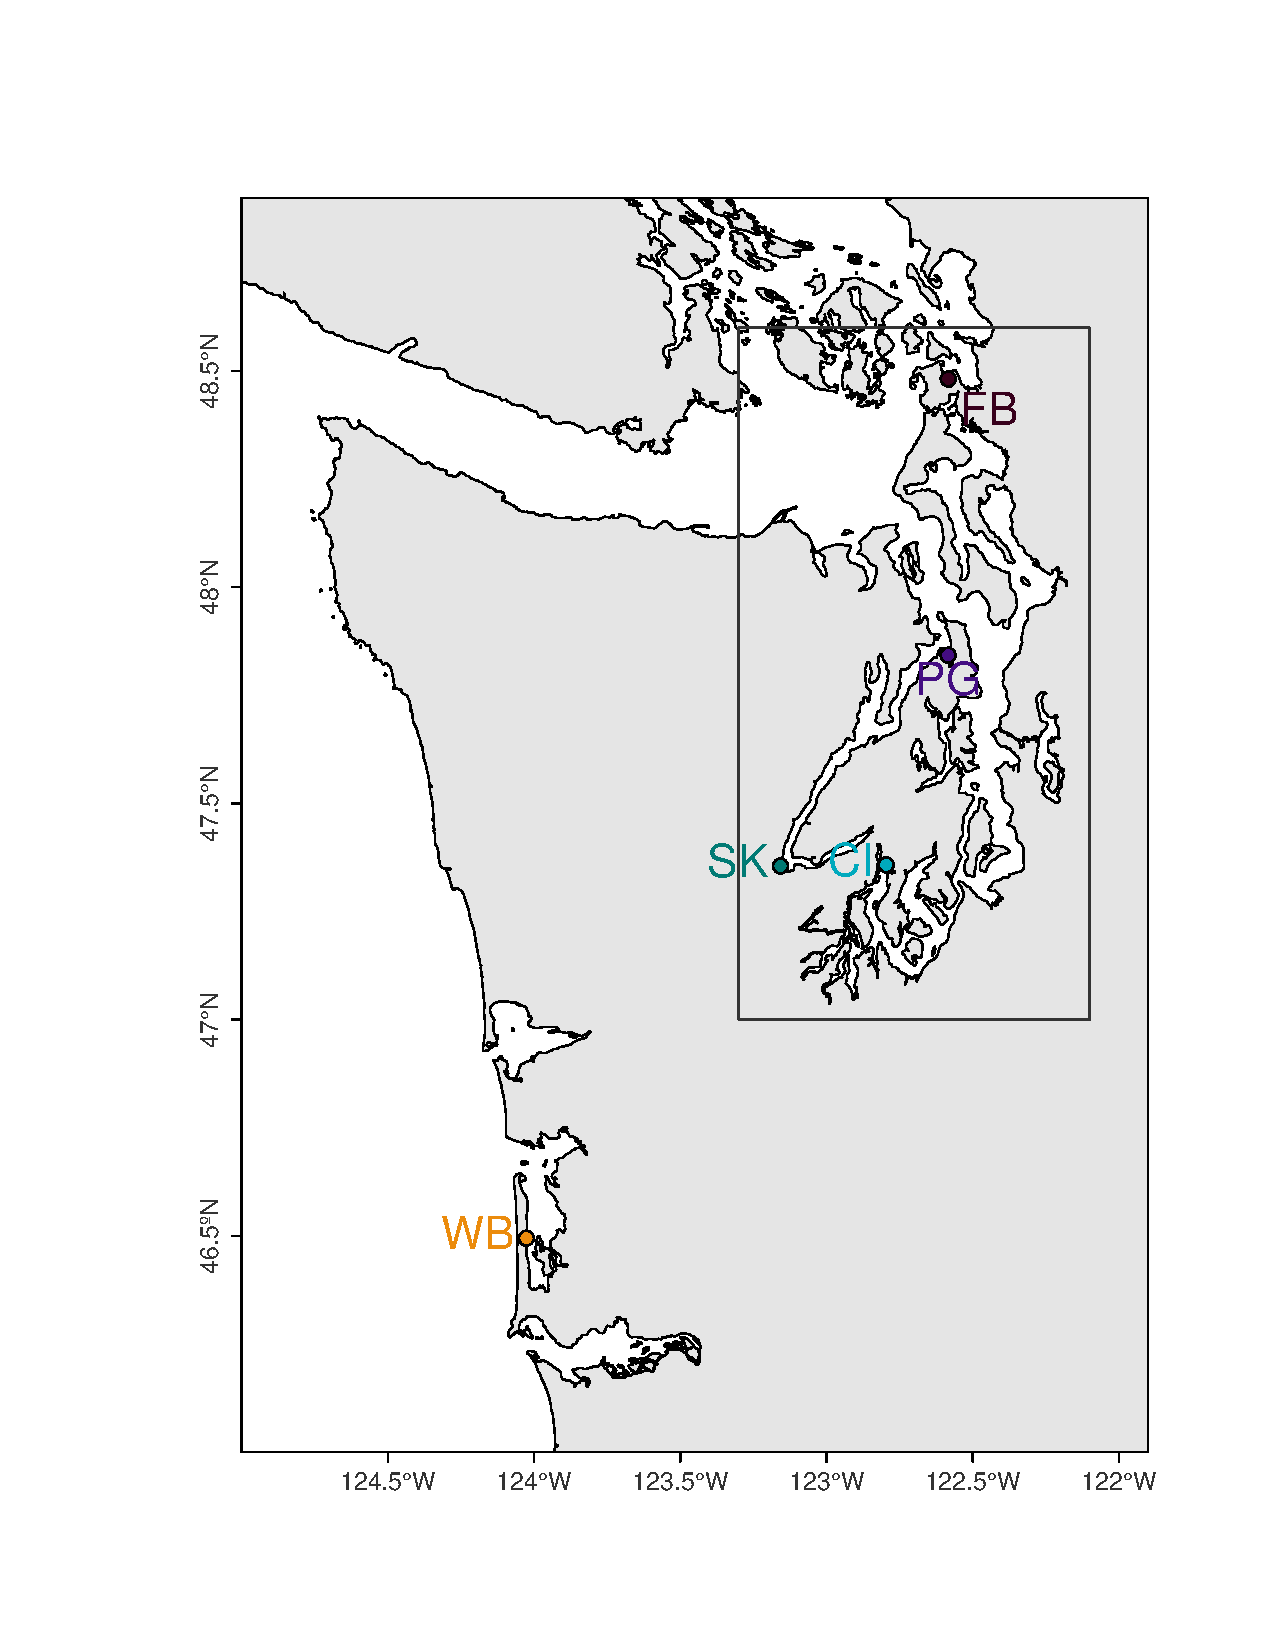
\includegraphics{figure/Ch1/fig1.1.pdf}
  \caption{Nitrogen pathways in soil}
  \label{fig:npathways}
\end{figure}
\clearpage

\textbf{Figure} \ref{fig:modIsotope}: Data (closed circles) and predicted values (open circles) for the model with the most support (Table \ref{tab:suppmod1}) for soil organic \(\delta^{15}N\) and \(\delta^{13}C\), \(\delta^{15}N\) of NH\textsubscript{4}\textsuperscript{+}, and C:N for both the salmon-enhanced and the salmondepleted banks of Hansen Creek at 1, 3, 6, 10, and 20 m from the edge of the creek bed with 95\% confidence intervals (dashed line) for predicted values. Blue (a and c) denotes measures of marine-derived nitrogen, and green (b and d) denotes site variable factors.\newline
\begin{figure}[h]
  \includegraphics[width=0.85\textwidth]{figure/Ch1/Figure2_Feddernetal.pdf}
  \caption{Data and predicted values for the model with the most support: Stable Isotopes}
  \label{fig:modIsotope}
\end{figure}
\clearpage

\textbf{Figure} \ref{fig:modConc}: Data (closed circles) and predicted values (open circles) for the model with the most support (Table \ref{tab:suppmod1}) for NH\textsubscript{4}\textsuperscript{+} and NO\textsubscript{3}\textsuperscript{-}, net mineralization and nitrification, {[}N\textsubscript{org}{]}, and gravimetric water content for both the salmon-enhanced and the salmon-depleted banks of Hansen Creek at 1, 3, 6, 10, and 20 m from the edge of the creek bed with 95\% confidence intervals (dashed line) for predicted values. Red (a, b, c, d) denotes measures of soil productivity, and green (e and f) denotes site variable factors.\newline 
\begin{figure}[h]
  \includegraphics[width=0.85\textwidth]{figure/Ch1/Figure3_Feddernetal.pdf}
  \caption{Data and predicted values for the model with the most support: Concentrations and Transformations}
  \label{fig:modConc}
\end{figure}
\clearpage

\textbf{Figure} \ref{fig:ch1resid}: Predicted verse observed values and predicted verse residuals for the model with the most support (Table \ref{tab:suppmod1}, Figure \ref{fig:modIsotope}, \ref{fig:modConc}) for each the response variables. \newline 
\begin{figure}[h]
  \includegraphics[width=1\textwidth]{figure/Ch1/ch1residuals.pdf}
  \caption{Residual Plots for Best Models}
  \label{fig:ch1resid}
\end{figure}
\hypertarget{stable-isotope-signatures-in-historic-harbor-seal-bone-link-food-web-assimilated-carbon-and-nitrogen-resources-to-a-century-of-environmental-change}{%
\chapter{Stable isotope signatures in historic harbor seal bone link food web-assimilated carbon and nitrogen resources to a century of environmental change}\label{stable-isotope-signatures-in-historic-harbor-seal-bone-link-food-web-assimilated-carbon-and-nitrogen-resources-to-a-century-of-environmental-change}}

\#\#Abstract

Anthropogenic climate change will impact nutrient cycles, primary production, and ecosystem structure in the world's oceans, although considerable uncertainty exists regarding the magnitude and spatial variability of these changes. Understanding how regional-scale ocean conditions control nutrient availability and ultimately nutrient assimilation into food webs will inform how marine resources will change in response to climate. To evaluate how ocean conditions influence the assimilation of nitrogen and carbon into coastal marine food webs, we applied a novel dimension reduction analysis to a century of newly acquired molecular isotope data derived from historic harbor seal bone specimens. By measuring bulk \(\delta^{13}C\) and \(\delta^{15}N\) values of source amino acids of these top predators from 1928-2014, we derive indices of primary production and nitrogen resources that are assimilated into food webs. We determined coastal food webs responded to climate regimes, coastal upwelling, and freshwater discharge, yet the strength of responses to individual drivers varied across the northeast Pacific. Indices of primary production and nitrogen availability in the Gulf of Alaska were dependent on regional climate indices (i.e., North Pacific Gyre Oscillation) and upwelling. In contrast, the coastal Washington and Salish Sea food webs were associated with local indices of freshwater discharge. For some regions (eastern Bering Sea, northern Gulf of Alaska) food web assimilated production was coupled with nitrogen sources, however other regions demonstrated no production-nitrogen coupling (Salish Sea). Temporal patterns of environmental indices and isotopic data from Washington state varied about the long-term mean with no directional trend. Data from the Gulf of Alaska, however, showed below average harbor seal \(\delta^{13}C\) values and above average ocean conditions since 1975, indicating a change in primary production in recent decades. Altogether, these findings demonstrate stable isotope data can provide useful indices of nitrogen resources and phytoplankton dynamics specific to what is assimilated by food webs.

\#\#Introduction

Changing ocean conditions are reshaping the structure and function of marine food webs on regional scales. Ocean temperature (\protect\hyperlink{ref-Hoegh2010}{Hoegh-Guldberg \& Bruno, 2010}), oxygen availability (\protect\hyperlink{ref-Brietburg2018}{Breitburg et al., 2018}), and climatic regimes such as El Niño Southern Oscillation (ENSO) (\protect\hyperlink{ref-Vecchi2010}{Vecchi \& Wittenberg, 2010}) alter nutrient availability and cycling, and thus, the ecological structure of marine systems. Projected global redistribution of nutrients suggests net primary production in the ocean is likely to change both spatially and temporally. Yet, substantial uncertainty remains, with predictions suggesting both increases and decreases in global net primary productivity of up to 20\% by 2100 (\protect\hyperlink{ref-Bopp2013}{Bopp et al., 2013}; \protect\hyperlink{ref-Gregg2003}{Gregg, Conkright, Ginoux, O'Reilly, \& Casey, 2003}; \protect\hyperlink{ref-Kwiatkowski2017}{Kwiatkowski et al., 2017}). An important contributor to this uncertainty is regional variability in phytoplankton response to ocean conditions and how that variability will impact other trophic levels and dependent fisheries (\protect\hyperlink{ref-Brander2010}{Brander, 2010}; \protect\hyperlink{ref-Moore2018}{J. K. Moore et al., 2018}). Ocean conditions (i.e., sea surface temperature, freshwater discharge, wind, and ice cover) have been associated with abundance and recruitment of many fish species in the Northeast Pacific (\protect\hyperlink{ref-Cunningham2018}{Cunningham, Westley, \& Adkison, 2018}; \protect\hyperlink{ref-Puerta2019}{Puerta, Ciannelli, Rykaczewski, Opiekun, \& Litzow, 2019}; \protect\hyperlink{ref-Stachura2014}{Stachura et al., 2014}). Nonetheless, these studies rarely include indicators of nutrient availability or primary production linking the ecosystem response to its environment. Understanding how regional and local scale physical drivers control nutrient availability and ultimately nutrient assimilation into food webs will be important for predicting the future availability of marine resources.

A strong empirical understanding of food web response to changing ocean conditions and nutrient constraints requires time series data that span multiple climate regimes to decouple natural variability with long-term anthropogenic changes. Currently, quantitative methods are also limited in their ability to scale primary production trends to ecosystem-level responses. Stable isotope measures of \(\delta^{15}N\) (\textsuperscript{15}N/\textsuperscript{14}N) of individual amino acids is an emerging tool for reconstructing trends in nitrogen sources from historic specimens (\protect\hyperlink{ref-McMahon2019}{McMahon et al., 2019}; \protect\hyperlink{ref-Sherwood2014}{Sherwood, Guilderson, Batista, Schiff, \& McCarthy, 2014}; \protect\hyperlink{ref-Sherwood2011}{Sherwood, Lehmann, Schubert, Scott, \& McCarthy, 2011}; \protect\hyperlink{ref-Whitney2019}{Whitney, Johnson, Dostie, Luzier, \& Wanamaker, 2019}). The \(\delta^{15}N\) signature at the base of the food web is primarily controlled by utilization and the isotopic signatures of different nitrogen sources, particularly urea, nitrate, and ammonium, by primary producers (\protect\hyperlink{ref-Graham2010}{2009}; \protect\hyperlink{ref-Ohkouchi2017}{Ohkouchi et al., 2017}). Measurements of bulk \(\delta^{15}N\) values from consumers can be difficult to attribute to changes at the base of the food web because trophic level shifts also effect the isotopic composition of bulk nitrogen (\protect\hyperlink{ref-Fry2006}{Fry, 2006}). Amino acid specific \(\delta^{15}N\) data addresses this challenge, as amino acids exhibit two distinct patterns in isotopic enrichment: trophic amino acids (i.e., glutamic acid, alanine, proline) become enriched in \(\delta^{15}N\) with each trophic transfer and source amino acids (i.e., phenylalanine, lysine, methionine) show minimal change and thus are reflective of the base of the food web (\protect\hyperlink{ref-Chikaraishi2009}{Yoshito Chikaraishi et al., 2009}; \protect\hyperlink{ref-McClelland2002}{McClelland \& Montoya, 2002}; \protect\hyperlink{ref-Ohkouchi2017}{Ohkouchi et al., 2017}).

Similar to the nitrogen stable isotope composition of amino acids as a proxy for nitrogen sources, carbon isotopic composition has emerged as a useful tool for assessing historic changes in phytoplankton (\protect\hyperlink{ref-Lorrain2020}{Lorrain et al., 2020}; \protect\hyperlink{ref-McMahon2019}{McMahon et al., 2019}). However, cellular growth rates, phytoplankton community composition, the isotopic composition of carbon in CO\textsubscript{2}, and CO\textsubscript{2} concentration all affect the \(\delta^{13}C\) (\textsuperscript{13}C/\textsuperscript{12}C) values of phytoplankton in tandem (\protect\hyperlink{ref-Burkhardt1999}{Burkhardt, Riebesell, \& Zondervan, 1999}; \protect\hyperlink{ref-Lorrain2020}{Lorrain et al., 2020}). The relative effects of these factors remain difficult to discern from carbon isotope data alone. Nonetheless, carbon stable isotope data is highly correlated with copepod biomass in the northeast Pacific and thus can be a useful combined index of ocean productivity (\protect\hyperlink{ref-Espinasse2020}{Espinasse, Hunt, Batten, Pakhomov, \& Tittensor, 2020}). While both source amino acid \(\delta^{15}N\) and bulk \(\delta^{13}C\) values can be influenced by a number of biogeochemical and physiological processes (Figure 2.1), they are useful indicators of nitrogen utilization (source amino acid \(\delta^{15}N\)) and phytoplankton dynamics (bulk \(\delta^{13}C\)), despite the difficulty in identifying specific mechanisms of fractionation.

Here we use source amino acid \(\delta^{15}N\) and bulk \(\delta^{13}C\) values of consumer bone collagen as indicators of change in food web-assimilated nitrogen (nitrogen utilization and isotopic composition at the base of the food web) and food web-assimilated production (phytoplankton composition, {[}CO\textsubscript{2}{]}, cellular growth, and physiology). These definitions assume major changes in nitrogen utilization and phytoplankton dynamics are recorded in the stable isotope composition of nitrogen and carbon in phytoplankton (\protect\hyperlink{ref-McMahon2019}{McMahon et al., 2019}; \protect\hyperlink{ref-Ohkouchi2017}{Ohkouchi et al., 2017}; \protect\hyperlink{ref-Sherwood2011}{Sherwood, Lehmann, Schubert, Scott, \& McCarthy, 2011}; \protect\hyperlink{ref-delaVega2021}{Vega et al., 2021}), scaled to the spatial and temporal resource use of consumers, and conserved with minimal trophic fractionation (\protect\hyperlink{ref-Chikaraishi2009}{Yoshito Chikaraishi et al., 2009}). Bulk \(\delta^{13}C\) and \(\delta^{15}N\) values of source amino acids such as phenylalanine (\(\delta^{15}N_{Phe}\)) from long-lived, generalist consumers provide ecosystem-level information of carbon and nitrogen dynamics that are integrated over space, time, and multiple energy pathways in the food web (\protect\hyperlink{ref-McCann2005}{McCann, Rasmussen, \& Umbanhowar, 2005}; \protect\hyperlink{ref-delaVega2021}{Vega et al., 2021}). As a result, these data sources are more relevant to questions of food web responses to large-scale environmental forcing than discrete measurements of inorganic nutrients or phytoplankton. Ultimately these data can be used to understand how ecosystems have responded to environmental variability in the past and glean insights into food web responses to oceanic conditions in the future.

Harbor seals (\emph{Phoca vitulina}) are a particularly well-suited predator to understand food web shifts through time because of their primarily piscivorous diet, generalist foraging strategies, high site fidelity, and frequent occurrence in museum specimen collections. Adult harbor seals typically forage 5 - 10 km from haul out sites and at depths \textless{} 200 m and are opportunistic feeders (\protect\hyperlink{ref-Lance2012}{Lance, Chang, Jeffries, Pearson, \& Acevedo-Gutiérrez, 2012}). Therefore, the nitrogen and carbon stable isotope composition of harbor seals offer a robust representation of the isotopic composition of carbon and nitrogen assimilated into coastal food webs. Harbor seal specific trophic enrichment factors for nitrogen have been quantified in controlled feeding studies, confirming minimal trophic enrichment for phenylalanine between seals and their prey (\protect\hyperlink{ref-Germain2013}{Germain, Koch, Harvey, \& McCarthy, 2013}). Environmentally induced shifts in foraging patterns, specifically nearshore verse offshore feeding, has the potential to affect the carbon isotope composition in harbor seal tissues (Figure 2.1). We assume these behavioral effects are minimal on annual time scales compared to changes in the carbon and nitrogen isotope composition at the base of the food web given their restricted foraging ranges.

We aim to identify how archived \(\delta^{15}N_{Phe}\) and bulk \(\delta^{13}C\) values vary regionally across the northeast Pacific on ecologically relevant scales (integrated annually and regionally) and through time using museum harbor seal specimens from 1928-2014 (Figure \ref{fig:map}). Additionally, we characterize abiotic factors that influence harbor seal \(\delta^{15}N_{Phe}\) and bulk \(\delta^{13}C\) values to identify ocean conditions important for food web assimilation of nitrogen and carbon. The effect of regional ocean condition on the stable isotope signature of source amino acids limits the application of short-term datasets for productivity studies, as short-term environmental perturbations are difficult to decouple from longer term trends such as climate regimes (\protect\hyperlink{ref-Vokshoori2014}{Vokhshoori \& McCarthy, 2014}). We therefore identify long-term environmental drivers that are important for interpreting reconstructed isotope data.

\#\#Methods
\#\#\#Sample Collection and Analysis

Harbor seal bone samples were obtained from specimens curated at the Burke Museum (University of Washington), the Slater Museum (University of Puget Sound), the Museum of the North (University of Alaska Fairbanks), the Royal British Columbia Museum, the Smithsonian Institute, and the National Marine Mammal Laboratory (NOAA). Specimens were either treated by maceration in warm water or cleaned by beetles and soaked in a dilute ammonia solution then stored in acid free boxes. Adult specimens were sampled from three regions: eastern Bering Sea, the Gulf of Alaska, and Washington state, which also included 18 specimens from the southern British Columbia coast (Figure \ref{fig:map}). We further stratified samples from the Gulf of Alaska into two subregions (northern and southeast) and Washington state into two subregions (coastal and Salish Sea) for a total of five subregions. Sampling prioritized long-term temporal coverage, specifically focusing on climate regimes shifts (i.e., PDO). Additionally, samples with sex and size metadata were prioritized, although it was not available for most specimens. Metadata was accessed through \href{http://www.vertnet.org/index.html}{VertNet} using catalogue numbers and institution codes.

Bone samples were decalcified with the resulting collagen acid hydrolyzed, derivatized, and analyzed for compound-specific nitrogen stable isotope analysis (CSIA) of 11 individual amino acids, including one source amino acid, phenylalanine (phe). Of the 11 amino acids, phenylalanine was the only discernable source amino acid and phenylalanine is the only amino acid data are reported in this manuscript (Appendix S1). CSIA samples were analyzed by GC-C-irMS at the University of Washington Facility for Compound-Specific Stable Isotope Analysis of Environmental Samples using a Thermo Scientific Trace GC + GC IsoLink coupled to a Delta V irMS following the procedures developed by \protect\hyperlink{ref-Chikaraishi2007}{Y. Chikaraishi, Kashiyama, Ogawa, Kitazato, \& Ohkouchi} (\protect\hyperlink{ref-Chikaraishi2007}{2007}) and protocols by Rachel Jeffrey's lab at University of Liverpool UK (full analytical details are provided in Appendix 1). Individual collagen samples were analyzed in triplicate along with a mixed amino acid standard of known isotopic composition (Sigma-Aldrich Co.) (mean precision of analytical standard for phenylalanine = 0.3‰). Internal and external standards were used and data processing included a drift correction. A total of 215 specimens were sampled from the time period of 1928-2014 for CSIA, making this the largest CSIA dataset of a mammal to date. Decalcified collagen of 190 specimens was analyzed for bulk \textsuperscript{13}C/\textsuperscript{12}C and bulk \textsuperscript{15}N/\textsuperscript{14}N at the University of Washington's IsoLab using a Costech ElementalAnalyzer, ConFlo III, MAT253 for continuous flow-based measurements. \textsuperscript{15}N/\textsuperscript{14}N and \textsuperscript{13}C/\textsuperscript{12}C are reported in standard delta notation:
\begin{equation} 
  \delta^{15}N_ ( \textperthousand vs. air) =   
  [(\frac{^{15}N/^{14}N_{Sample}}{^{15}N/^{14}N_{Air}} -1)*1000]
  \label{eq:deltN}
\end{equation}
\begin{equation} 
  \delta^{13}C_ ( \textperthousand vs. VPBD) =   
  [(\frac{^{13}C/^{13}C_{Sample}}{^{13}C/^{13}C_{VPBD}} -1)*1000]
  \label{eq:deltC}
\end{equation}
Internal laboratory standards (Bristol Bay salmon and glutamic acid) were interspersed with samples for a two-point calibration and blank correction (mean standard precision 0.09‰ for \(\delta^{15}N\) and 0.04‰ for \(\delta^{13}C\)). A linear drift correction was also applied using IsoDat software. The collagen C:N ratio was used to verify the integrity of collagen for stable isotope analysis following specimen treatment and storage (\protect\hyperlink{ref-vanKlinken1999}{Klinken, 1999}).

The isotopic composition of marine dissolved organic carbon has been steadily depleted in \textsuperscript{13}C over the past 100 years due to increases in anthropogenic CO\_2 in the atmosphere (referred to as the Oceanic Seuss Effect) (\protect\hyperlink{ref-Quay1992}{Quay, Tilbrook, \& Wong, 1992}). \(\delta^{13}C\) data were therefore corrected for the Seuss Effect using the following equation (\protect\hyperlink{ref-Misarti2009}{Misarti, Finney, Maschner, \& Wooller, 2009}):
\begin{equation} 
 \mbox {Seuss Effect Correction Factor} =   
  d * e^{0.027*(t-1850)}
  \label{eq:seuss}
\end{equation}
Where \emph{d} is the maximum annual rate of \(\delta^{13}C\) decrease specific to the North Pacific (-0.014 derived from \protect\hyperlink{ref-Quay1992}{Quay, Tilbrook, \& Wong} (\protect\hyperlink{ref-Quay1992}{1992})), \emph{t} is the year represented by the year of specimen collection with a one-year lag. The Seuss effect varies regionally (\protect\hyperlink{ref-Tagliabue2008}{Tagliabue \& Bopp, 2008}) and we applied a northeast Pacific parameterization (\protect\hyperlink{ref-Misarti2009}{Misarti, Finney, Maschner, \& Wooller, 2009}).

Standard linear models were used to identify whether size (standard length, cm), sex, and subregion of the harbor seals sampled were related to isotopic composition and to test whether these parameters needed to be standardized in environmental models. \(\delta^{15}N_{Phe}\) and \(\delta^{13}C\) values were modelled independently as univariate continuous response variables using the following equation:
\begin{equation} 
 y_i \sim N(\boldsymbol{\alpha} + \boldsymbol{\beta X}_i, \sigma^2_y)
  \label{eq:linmods}
\end{equation}
where \emph{y} is the mean triplicate value for each individual \emph{i} for either \(\delta^{15}N_{Phe}\) or \(\delta^{13}C\) values. \textbf{X} represents the matrix of predictors (sex, length, subregion), \(\boldsymbol{\alpha}\) is a scalar and \(\boldsymbol{\beta}\) is a vector of coefficients for the predictors. Length (n = 116) was modelled as a continuous variable and was natural log transformed; subregion and sex (n = 190) were modelled as factors. Individual models were used to test whether a predictor was significant as opposed to a multivariate framework because, 1) sample sizes for \(\delta^{15}N_{Phe}\) (n = 215) and \(\delta^{13}C\) (n = 190) data varied, and 2) predictor metadata was incomplete for specimens. A pairwise t-test using the Bonferroni correction and non-pooled standard deviation was also used to compare differences in mean isotope signature between subregions and sex (Figure \ref{fig:dist}, Tables \ref{tab:ttestN} \& \ref{tab:ttestC}).

To understand the extent of coupling between indices of food web assimilated production and nitrogen resources, a linear model representing the basin wide relationship was fit to \(\delta^{15}N_{Phe}\) and \(\delta^{13}C\) values as continuous variables assuming normal errors. To understand spatial variation in this relationship, a hierarchical model was fit to the same dataset with varying slope and varying intercept based on subregion as a random effect. This model took the following form:
\begin{equation} 
 y_i \sim N(\boldsymbol{\alpha}_{j[i]} + \boldsymbol{\beta}_{j[i]}\boldsymbol{x}_i, \sigma^2_y)
  \label{eq:hiermods}
\end{equation}
Where \emph{y} represents \(\delta^{13}C\) values as a continuous variable and x represents \(\delta^{15}N_{Phe}\) values as a continuous variable and j represents the group level predictor, subregion. \(\boldsymbol{\alpha}\) and \(\boldsymbol{\beta}\) are each vectors of coefficients that vary by subregion.

\#\#\#Quantifying effects of ocean condition on food web isotope indices

Linear models were used to identify environmental drivers of \(\delta^{13}C\) and \(\delta^{15}N_{Phe}\) values using a suite of environmental indices as covariates. A total of 42 environmental time series were compiled as potential predictor variables (Table 2.2) based on previous evidence for food web importance in the northeast Pacific (\protect\hyperlink{ref-DiLorenzo2008}{Di Lorenzo et al., 2008}; \protect\hyperlink{ref-Stachura2014}{Stachura et al., 2014}). Each environmental time series was standardized around a mean of 0 and standard deviation of 1 and discharge data was also natural log transformed. We divided these environmental covariates a priori into four main mechanistic properties based on the expected effect on nutrient assimilation into the food web: climate regime, freshwater discharge, circulation (wind and upwelling), and sea surface temperature (Figure 2.1). Given the three regions in our analysis, each of these hypotheses were also divided according to our regional geographic breaks (eastern Bering Sea, Gulf of Alaska, and Washington). To reduce collinearity between environmental time series and reduce the total number of candidate models, a subset of 7 environmental times series were selected for each region based on the temporal overlap with stable isotope data. Each subset contained at least one time series for each of the four mechanistic properties and all possible combinations of predictors were tested (Table 2.3). While reduction of the number of times series provides analytical benefits, it comes at the cost of potentially conservative estimates of which covariates are important, meaning important components of ocean condition to the food webs may be missed.

\(\delta^{15}N_{Phe}\) and \(\delta^{13}C\) values were independently considered as response variables to evaluate relationships between predictors (environmental indices and location) and stable isotope data using Figure \eqref{eq:linmods} where X is a matrix of predictors using the 7 standardized environmental time series (continuous) and subregion (factor) as covariates. We treated carbon and nitrogen isotopes as response variables separately in linear models, rather than in a combined multivariate model due to differences in sample size and differences in the strength of correlation between for \(\delta^{15}N_{Phe}\) and \(\delta^{13}C\) values for each subregion. Time series data prior to 1950 and after 2014 was excluded from this analysis as data for some covariates did not extend beyond 1950. Candidate models (n = 53) were compared using Akaike Information Criteria with a small sample size correction {[}AICc{]} and included all combinations of the environmental indices. In addition, a subregion factor was included with two levels for Washington (Salish Sea and coastal Washington) and the Gulf of Alaska (southcentral and southeast) and a null model (intercept only) was also tested. Tissue turnover time of bone collagen has not been measured in mammals of this size to our knowledge but is approximately 173 days for birds (\protect\hyperlink{ref-Hobson1992}{Hobson \& Clark, 1992}). Thus, a lag of one year was applied to the stable isotope datasets to account for the timing of tissue turnover in bone collagen. To validate this approach of applying a 1-year lag, 0- and 2-year lags were also applied to the best models of each region an compared to the 1-year lag using AIC. Additionally, month was tested as a smoothed predictor with 12 knots for stable isotope data in Washington samples using a generalized additive model (GAM). Support for a significant smoothing term would identify and seasonality in the data, which would be expected if tissue turnover time is less than a year. A one-year tissue turnover time was confirmed as a suitable assumption for harbor seal bone collagen, as 0- and 2- year lags had similar or less model support. There was no support for a smoothing effect by month in generalized additive models of \(\delta^{15}N_{Phe}\) and \(\delta^{13}C\) which would have indicated any seasonal variability in isotope composition and thus a turnover time of less than or greater than a year (p \textless{} 0.05; Figure \ref{fig:Length}) and thus a 1-year lag was applied to isotope data for all temporal analyses.

For each model with relatively high support (ΔAICc \textless{} 2) the AICc weight and the coefficient for each covariate is reported (Figure \ref{fig:dist}. To confirm collinearity was not problematic in the candidate models that included more than one environmental covariate, matrix scatterplots and variance inflation factors (vif) were used from the car package (Fox et al.~2019) in R (R Development Core Team, 2020).

\#\#\#Gaussian Process Dynamic Factor Analysis (GPDFA)
To further understand how the environment, \(\delta^{13}C\), and \(\delta^{15}N_{Phe}\) values covary through time in the Northeast Pacific, we developed a novel extension of conventional Dynamic Factor Analysis (DFA). DFA is a dimension reduction technique that identifies common processes underlying a set of multivariate time series. This technique has been applied to multivariate time series problems in fisheries and ecology to identify patterns of oceanographic variability that drive Pacific salmon stocks (\protect\hyperlink{ref-Jorgensen2016}{Jorgensen, Ward, Scheuerell, \& Zabel, 2016}; \protect\hyperlink{ref-Ohlberger2016}{Ohlberger, Scheuerell, Schindler, \& Peters, 2016}; \protect\hyperlink{ref-Stachura2014}{Stachura et al., 2014}).

DFA models identify common trends across multiple time series (``latent trends'') and estimates the importance of that trend for each individual time series as a coefficient (``factor loading''). The two equations describing DFA take on the following form:
\begin{equation} 
 \boldsymbol{y}_t = \boldsymbol{Zx}_t + \boldsymbol{v}_t,\mbox{ where }\boldsymbol{v}_t \sim MVN(0,\boldsymbol{R})
  \label{eq:gdfa1}
\end{equation}
\begin{equation} 
 \boldsymbol{x}_t = \boldsymbol{x}_{t-1} + \boldsymbol{w}_t,\mbox{ where }\boldsymbol{w}_t \sim MVN(0,\boldsymbol{I})
  \label{eq:gdfa2}
\end{equation}
The observed data \textbf{y}\textsubscript{t} are modeled as combinations of latent trends \textbf{x}\textsubscript{t} at time \emph{t} (the dimensions of \textbf{x}\textsubscript{t} matching the number of trends which are also referred to as states) and factor loadings (\textbf{Z}) (a coefficient for each time series for each trend) at time \emph{t}, which are modeled as a random walk (Zuur et al.~2003). In addition there is an optional random observation error (\textbf{v}\textsubscript{t}) and process error (\textbf{w}\textsubscript{t}) which are multivariate normal

Our extension of DFA adopts an alternative model of the latent trends, modeling them with Gaussian Processes rather than random walks.Gaussian Processes (GP) have been widely used in fisheries and other fields (\protect\hyperlink{ref-Munch2018}{Munch, Giron‐Nava, \& Sugihara, 2018}). Instead of modeling a time series as an autoregressive process, GPs model a time series via a mean and variance function, \emph{x\textasciitilde{}}\(MVN(u,\Sigma)\) where \emph{u} represents and optional mean vector and \textbf{Σ} a covariance matrix. For GPDFA, we assume the mean to be zero, letting just the covariance function determine the GP smoothing. GPs are flexible in that the covariance matrix can be described by a wide range of flexible functions; for this application we use a Gaussian kernel (squared exponential) so that \(\Sigma_{i,j}=\sigma^2 exp(-d_{i,j}/\sigma)\), where \(\sigma^2\) is a variance parameter controlling the magnitude, θ is a shape parameter controlling how quickly covariance declines, and \(d_{i,j}\) is the known distance between time points \emph{i} and \emph{j}. A benefit of modeling \textbf{Σ} with a covariance function is that regardless of the dimensionality, all elements of \textbf{Σ} can be described by a small number of parameters. For GPDFA, we choose to use a GP predictive process model, because the number of time points may be large (\protect\hyperlink{ref-Latimer2009}{Latimer, Banerjee, Sang Jr, Mosher, \& Silander Jr, 2009}). This predictive model estimates the function values at a subset of locations (knots), and combines these estimates with the distance to locations at which data are observed to make predictions. More specifically, the values of the time series at the knot locations are \(x^*\)\textasciitilde{}\(MVN(0,\Sigma^*)\). Given the known distances between the locations of knots and locations of data, the covariance matrix between the two can be calculated, \(\Sigma_{(x,x^*)}\). Finally, the predictions of the time series at the observed data can be calculated as \(\hat{x}=\Sigma'_{(x,x^*)}\Sigma^{*-1}x^*\). In this extension of DFA, all other model components are identical to the conventional time series version with latent trends modeled as a random walk.

With the Gaussian Process DFA model, a decision needs to be made a priori about selecting the number and location of knots, where the function parameters are estimated at. There are multiple approaches for doing this; we adopted a model with 15 knots (more knots resulting in a smoother function), and estimated the knot location by performing a clustering approach of the years corresponding to the raw observations (partitioning around medoids, using the `pamk' function in the fpc library in R).

With conventional DFA using an autoregressive model, long gaps in time series data result in large, overestimations of the variance of the latent trends. Gaussian Processes model time series as a multivariate normal distribution, with estimated mean vector \textbf{u} and covariance matrix \textbf{Σ} (\protect\hyperlink{ref-Munch2018}{Munch, Giron‐Nava, \& Sugihara, 2018}). To constrain the number of estimated parameters, elements of \textbf{Σ} were modeled with a Gaussian or squared covariance exponential function such that \(\Sigma_{(i,j)}= \sigma^2 exp(-(t_i-t_j )^2/\theta)\). In this parameterization, \(\sigma^2\) controls the variability of the stochastic process, \(\theta\) controls the rate of decay in correlation between time steps, and t\textsubscript{i} and t\textsubscript{j} are the time variables (e.g.~years) for locations \emph{i} and \emph{j}.

We considered models with 1- 4 underlying trends. Each trend was modelled separately (different means) but models with multiple trends to have a shared covariance matrix amongst trends. The GPDFA approach was applied to time series from each region and the best model was selected using leave-one-out cross-validation (LOOIC) from the loo package in R (\protect\hyperlink{ref-Vehtari2017}{Vehtari, Gelman, \& Gabry, 2017}). The choice of knots affects the degree of smoothness, with more knots creating more smooth functions. We tested several different numbers of knots and found results to be qualitatively similar. Similar to the previous analysis, time series data prior to 1948 for Washington state and prior to 1940 and after 2008 for the Gulf of Alaska was excluded from this analysis. We fit GPDFA to data from each region including all of the initial 42 identified environmental time series for that region (Table 2.2), \(\delta^{15}N_{Phe}\) and \(\delta^{13}C\) values, with location as a factor. We implemented GPDFA using the Stan language (Stan Development Team 2019, \protect\hyperlink{ref-Carpenter2017}{Carpenter et al., 2017}), and R (R Core Development Team 2019, version 3.6.2) via R package rstan (Stan Development Team 2019, version 2.21.2). Code to implement GPDFA is available \href{https://github.com/mfeddern/CSIA-AA/blob/master/SourceData/Src/Analysis/gpdfa.stan}{here}

\#\#Results

\(\delta^{15}N_{Phe}\) and bulk \(\delta^{13}C\) values did not vary by sex (p \textgreater{} 0.05, Figure \ref{fig:dist} or size for the individuals sampled (p \textgreater{} 0 .05; Figure \ref{fig:Length}). Spatial variation in harbor seal \(\delta^{15}N_{Phe}\) and \(\delta^{13}C\) values were observed on subregional scales. \(\delta^{15}N_{Phe}\) values were similar for harbor seals in the northern Gulf of Alaska (11.9 ± 2.9, mean ± 1SD), southeast Gulf of Alaska (10.8 ± 1.7), and coastal Washington (11.3 ± 1.9). The eastern Bering Sea had significantly higher \(\delta^{15}N_{Phe}\) values compared to other subregions (15.2 ± 1.8) followed by the Salish Sea (12.2 ± 2.3) which had similar \(\delta^{15}N_{Phe}\) values compared to the northern Gulf of Alaska (Figure \ref{fig:dist}, Table \ref{tab:ttestN}). \(\delta^{13}C\) values varied by subregion (p \textless{} 0.05) with the exception of the Gulf of Alaska, where the northern (-14.6 ± 0.9) and southeast (-14.4 ± 1.1) subregions were not significantly different, and the eastern Bering Sea (-13.4 ± 0.9) and coastal Washington (-13.6 ± 0.9) were not significantly different (Figure \ref{fig:dist}, Table \ref{tab:ttestC}). The variation between subregions appeared to follow a latitudinal gradient, where harbor seal mean \(\delta^{13}C\) values were most enriched in \(^{13}C\) in the Salish Sea (-12.2 ± 1.5), became more depleted from coastal Washington and into the Gulf of Alaska (Table \ref{tab:ranges}).

The relationship between harbor seal \(\delta^{15}N_{Phe}\) and \(\delta^{13}C\) values also varied on subregional scales. There was positive linear association between harbor seal \(\delta^{15}N_{Phe}\) and \(\delta^{13}C\) values in the combined northeast Pacific basin and Bering Sea model with a slope of 0.12 (Figure \ref{fig:hiermod}A). For the hierarchical subregion model, the eastern Bering Sea and coastal Washington demonstrated similar relationship, with slopes of 0.08 (95\% CI {[}0.05, 0.11{]}) and 0.07 (95\% CI {[}0.05, 0.09{]}) respectively. Similarly, harbor seals in both Gulf of Alaska subregions demonstrated comparable coupling of \(\delta^{15}N_{Phe}\) and \(\delta^{13}C\), with slopes of 0.13 (95\% CI {[}0.11, 0.14{]}) for the northern subregion and 0.12 (95\% CI {[}0.10, 0.14{]}) for the southeastern subregion. Salish Sea harbor seals had a distinct relationship between \(\delta^{15}N_{Phe}\) and \(\delta^{13}C\) values relative to other subregions with a slope of only 0.02 that was not significantly different from 0 (95\% CI {[}0.0, 0.04{]}) (Figure \ref{fig:hiermod}B).

For both \(\delta^{15}N_{Phe}\) and \(\delta^{13}C\) values there was substantial support for models including environmental indices rather than null or subregion only models. The relationship between environmental indices and harbor seal \(\delta^{15}N_{Phe}\) and \(\delta^{13}C\) values in the northeast Pacific varied on regional scales. For Washington, the best model to predict harbor seal \(\delta^{15}N_{Phe}\) values included Columbia River discharge in high flow months, summer upwelling, and subregion. There was substantial model uncertainty for \(\delta^{15}N_{Phe}\) values in the Washington region, however 90\% of model weight supported the inclusion of Columbia River discharge (Figure \ref{fig:coefres}A). The model for harbor seal \(\delta^{13}C\) values with the most support indicated a positive association between PDO, spring upwelling, and freshwater discharge in the Washington region (Figure \ref{fig:coefres}B). In the Gulf of Alaska, the summer upwelling model had the most support as a predictor of harbor seal \(\delta^{15}N_{Phe}\) values with some model support for inclusion of the NPGO (North Pacific Gyre Oscillation), although the coefficients for this covariate did not differ substantially from 0 (Figure \ref{fig:coefres}C). The best model for harbor seal \(\delta^{13}C\) values for the Gulf of Alaska included subregion, PDO (Pacific Decadal Oscillation), and NPGO (Figure \ref{fig:coefres}D). In contrast to Washington, the Gulf of Alaska models supported a negative association between δ13C values and PDO. The null model for \(\delta^{15}N_{Phe}\) values in the eastern Bering Sea had the most support (Figure \ref{fig:coefres}E). Lack of model support for environmental covariates in the eastern Bering Sea may have been a result of the small sample size in the region. Cross-shelf wind was included as a predictor in the best model (Figure \ref{fig:coefres}F) for \(\delta^{13}C\) values in the eastern Bering Sea and was supported by 76\% of the model weight.

PDO and Kuskokwim river discharge during high flow months were found to be highly collinear (VIF \textgreater{} 10) and PDO was omitted from the candidate model set for the eastern Bering Sea analysis. All other models containing multiple environmental predictors with relative support had variance inflation factors of less than 2 indicating only moderate collinearity across covariates. Model residuals for the best models did not show trends through time (Figure \ref{fig:linresid}). This indicates that there were no trends associated with other potential ecosystem changes, such as harbor seal foraging strategy for example, after accounting for ocean condition. Model results did not change when using \(\delta^{13}C\) data that were not corrected for the regional Seuss Effect.

The GPDFA analysis showed temporal synchronies and shared trends across environmental conditions and stable isotope values in the northeast Pacific. In the Gulf of Alaska, the data supported three latent trends (Figure \ref{fig:GDFAAK}). Both \(\delta^{15}N_{Phe}\) and \(\delta^{13}C\) values had the highest loadings for trend 1, which showed an increase starting in 1965 until 1980 followed by the trend oscillating at approximately 25\% above the long-term average. The harbor seal \(\delta^{15}N_{Phe}\) values for the southeast subregion, harbor seal \(\delta^{13}C\) values, and spring upwelling had negative loadings on trend 1; loadings of \(\delta^{15}N_{Phe}\) values were generally weaker relative to loadings of \(\delta^{13}C\) values. For the other two trends (2-3), loadings were clustered by environmental driver category. Latent trend 2 oscillated around the long-term average and was uninformative. Trend 3 was below average starting in 1985 with strong loadings for climate time series, spring and summer upwelling, and discharge in high flow months (Figure \ref{fig:GDFAAK}). Annual discharge, autumn upwelling, Oceanic Niño Index and Northern Oscillation Index did not demonstrate strong loadings for any trend. In Washington, there was support for two latent trends. Latent trend 1 shows a rapid increase in the 1940's to 25\% above the long-term mean then a gradual decline until 1986 to approximately 40\% below the long-term mean, with values below the mean starting in 1977 (Figure \ref{fig:GDFAWA}). Trend loadings for harbor seal \(\delta^{15}N_{Phe}\) and \(\delta^{13}C\) values were stronger for coastal seals and trend 1 had stronger loadings for freshwater discharge than trend 2. Trend 2 had strong loadings for \(\delta^{15}N_{Phe}\) and \(\delta^{13}C\) values for both Salish Sea and coastal Washington harbor seals. Trend 2 oscillated above and below the long-term mean and had large loadings for sea surface temperature, summer upwelling, Fraser River discharge and climate indices (Figure \ref{fig:GDFAWA}).

To validate this approach of applying a 1-year lag, 0- and 2-year lags were also applied to the best models of each region an compared to the 1-year lag using AIC. Additionally, month was tested as a smoothed predictor with 12 knots for stable isotope data in Washington samples using a generalized additive model (GAM). Support for a significant smoothing term would identify and seasonality in the data, which would be expected if tissue turnover time is less than a year. A one-year tissue turnover time was confirmed as a suitable assumption for harbor seal bone collagen, as 0- and 2- year lags had similar or less model support. There was no support for a smoothing effect by month in generalized additive models of \(\delta^{15}N_{Phe}\) and \(\delta^{13}C\) which would have indicated any seasonal variability in isotope composition and thus a turnover time of less than or greater than a year (p \textless{} 0.05; Figure \ref{fig:Length}) and thus a 1-year lag was applied to isotope data for all temporal analyses.

\#\#Discussion

We analyzed bone collagen \(\delta^{15}N_{Phe}\) and bulk \(\delta^{13}C\) values from harbor seal museum specimens collected between 1928 and 2014 as indices of change in food web assimilated nitrogen and carbon. Based on previous research (\protect\hyperlink{ref-Lorrain2020}{Lorrain et al., 2020}; \protect\hyperlink{ref-Sherwood2014}{Sherwood, Guilderson, Batista, Schiff, \& McCarthy, 2014}; \protect\hyperlink{ref-delaVega2019}{Vega, Jeffreys, Tuerena, Ganeshram, \& Mahaffey, 2019}), we interpret \(\delta^{15}N_{Phe}\) and bulk \(\delta^{13}C\) values as primarily representing nitrogen and carbon resource utilization, and growth and community composition of primary producers at the base of the food web. Our data show the relationship between indices of primary production and nitrogen resources assimilated into food webs varies regionally across the northeast Pacific. By pairing these data with environmental time series data, we provide new insights into large scale environmental forcing that impacts the base of the food web and is transferred to higher trophic levels. Specifically, oceanic conditions associated with climate regimes and upwelling explain significant temporal variation in \(\delta^{15}N_{Phe}\) and bulk \(\delta^{13}C\) values of coastal predators in northeast Pacific (Figure \ref{fig:coefres}; Figure \ref{fig:linresid}). This analysis demonstrates \(\delta^{15}N_{Phe}\) and bulk \(\delta^{13}C\) values are useful indicators of resources assimilated by coastal food webs.

\#\#\#Spatial variation in stable isotope indices

The geographically widespread association between harbor seal \(\delta^{15}N_{Phe}\) and bulk \(\delta^{13}C\) values indicates food web assimilated primary production is coupled with nitrogen resources in most regions of the northeast Pacific, with the Salish Sea as a notable exception (Figure \ref{fig:hiermod}). Short-term studies in coastal Washington showed phytoplankton respond considerably to nitrogen inputs and are frequently nitrogen limited (\protect\hyperlink{ref-Dortch1989}{Dortch \& Postel, 1989}; \protect\hyperlink{ref-Kudela2009}{R. M. Kudela \& Peterson, 2009}). Similarly, short term studies of the inner Gulf of Alaska shelf demonstrated primary production is generally nitrogen limited, and size, growth rates, and community composition are all tightly coupled with nutrient availability (\protect\hyperlink{ref-Strom2006}{Strom, Olson, Macri, \& Mord, 2006}). A significant relationship between bulk \(\delta^{15}N\) and \(\delta^{13}C\) values was also observed in the tissues of some gorgonian corals over the same time period in coastal Gulf of Alaska (\protect\hyperlink{ref-Williams2007}{Williams, Risk, Stone, Sinclair, \& Ghaleb, 2007}). Given the evidence of nitrogen limitations and its relationship with phytoplankton growth and community composition in these coastal environments, the association between \(\delta^{15}N_{Phe}\) and bulk \(\delta^{13}C\) values could be the result of nitrogen limiting growth at the base of the food web. Alternatively, the \(\delta^{15}N_{Phe}\) and bulk \(\delta^{13}C\) coupling could be driven by covariance with an untested environmental variable that impacts most of the northeast Pacific but not the Salish Sea.

The coastal Washington and the Salish Sea food webs assimilate different nitrogen and carbon sources (Figure \ref{fig:coefres} A \& B). Salish Sea harbor seals have higher \(\delta^{15}N_{Phe}\) and bulk \(\delta^{13}C\) values compared to individuals on the outer coast, which is likely due to significant contributions of intertidal producers and the legacy of anthropogenic N in the Salish Sea food web. Intertidal macrophytes (seagrass and algae) have similar δ13C values (\textasciitilde{} -10‰) compared to harbor seals in the Salish Sea, while other potential sources are much lower (i.e., marine derived sources \textasciitilde{} -20‰, terrestrial derived sources \textasciitilde{} -30‰) (\protect\hyperlink{ref-Conway2015}{Conway-Cranos et al., 2015}; \protect\hyperlink{ref-Howe2015}{Howe \& Simenstad, 2015}). Incorporation of intertidal producers into the Salish Sea food web explains the difference in carbon stable isotope signatures between Salish Sea and coastal Washington harbor seals (\textasciitilde1.4‰, Figure \ref{fig:coefres}A). However, it does not explain the higher \(\delta^{15}N_{Phe}\) values (Figure \ref{fig:coefres}B, Table \ref{tab:ranges}). Surface nitrate was observed to be 8‰ -- 12‰ off the coast of Washington in spring 1993 (\protect\hyperlink{ref-Wu1997}{Wu, Calvert, \& Wong, 1997}) which was exceeded by harbor seals in both coastal Washington and the Salish Sea (Table \ref{tab:ranges}). It is likely anthropogenically derived nitrogen sources contribute to the higher observed \(\delta^{15}N_{Phe}\) values both directly and indirectly, particularly in the Salish Sea where harbor seal \(\delta^{15}N_{Phe}\) values were up to 2.4‰ higher than coastal Washington seals. Wastewater treatment facilities and agriculture runoff contribute substantial amounts (\textasciitilde32\%) of nitrogen in the Salish Sea (Mohamedali et al.~2011) and are enriched in \(^{15}N\). In recent decades, Salish Sea waters have also been characterized by low dissolved oxygen and hypoxic events (PSEMP 2019) from human derived nitrogen loading. Anoxic conditions are conducive to denitrification, another potential indirect source of \(^{15}N\) from human activities in the region.

\#\#\#Ocean condition and stable isotope indices

Washington state food webs exhibit environmentally induced changes in assimilated primary production and nitrogen sources. The isotope-ocean condition relationship in the region can be explained by introduction of terrestrial derived nutrients and climatically induced changes in phytoplankton community structure observed in previous studies (\protect\hyperlink{ref-Du2014}{Du \& Peterson, 2014}; \protect\hyperlink{ref-Kudela2008}{R. Kudela et al., 2008}; \protect\hyperlink{ref-Du2015}{Xiuning, William, \& Linda, 2015}). For example, the PDO has been associated with phytoplankton community shifts between dinoflagellates and diatoms in the northern California Current (\protect\hyperlink{ref-Du2015}{Xiuning, William, \& Linda, 2015}). Similarly, the phytoplankton community composition is distinct in the early (spring) upwelling season compared to the late (summer) upwelling season (\protect\hyperlink{ref-Du2014}{Du \& Peterson, 2014}). This could explain the inversely related associations between bulk \(\delta^{13}C\) values and summer and spring upwelling (Figure \ref{fig:coefres}B). Shifts in phytoplankton community structure are therefore a mechanism to explain the relationship between harbor seal bulk \(\delta^{13}C\) values and ocean condition. In addition, freshwater discharge explains 16\% of variation observed in both \(\delta^{15}N_{Phe}\) and bulk \(\delta^{13}C\) values in Washington. The Columbia River Plume introduces terrestrial derived nutrients, including nitrogen, and has been associated with increased primary production and fish production (\protect\hyperlink{ref-Kudela2008}{R. Kudela et al., 2008}). The covariation between \(\delta^{15}N_{Phe}\), bulk \(\delta^{13}C\), and discharge indicates isotopically distinct nitrogen resources introduced by freshwater discharge alters primary production which is then assimilated into the Washington food web, and ultimately harbor seals.

In the eastern Bering Sea, our results suggest ice-born algae and \(^{15}N\) enriched nitrogen from the inner shelf are important for supporting the coastal food web. Recent evidence supports that consumer \(\delta^{15}N_{Phe}\) values reflect nitrate \(\delta^{15}N\) values in the arctic (de la Vega et al.~2020). However, our \(\delta^{15}N_{Phe}\) values from harbor seals of the eastern Bering Sea were high relative to previous studies of summer nitrate (5 to 9‰) (\protect\hyperlink{ref-Lehmann2005}{Lehmann et al., 2005}) and plankton nitrogen isotope signatures (6-12‰) (\protect\hyperlink{ref-Smith2002}{Smith, Henrichs, \& Rho, 2002}) from the outer and mid Bering Sea shelf. \protect\hyperlink{ref-Morales2014}{Morales et al.} (\protect\hyperlink{ref-Morales2014}{2014}) subsequently found the stable isotope composition of nitrogen in diatoms ranged from 5-21‰ in late winter and early spring. These values also increased in association to sea ice with a positive shoreward gradient (\protect\hyperlink{ref-Morales2014}{Morales et al., 2014}). The range of sea-ice algae \(\delta^{15}N\) values observed by \protect\hyperlink{ref-Morales2014}{Morales et al.} (\protect\hyperlink{ref-Morales2014}{2014}) are consistent with our observed \(\delta^{15}N_{Phe}\) values in harbors seals (\ref{tab:ranges}). Furthermore, the harbor seals in this study were located near the inner shelf in an area that has been partially covered by sea ice from January to May during the past century (\protect\hyperlink{ref-Stabeno2007}{Stabeno, Bond, \& Salo, 2007}). Together this indicates ice algae as a significant contributor to the coastal food web. The disconnect between the \(\delta^{15}N\) values of offshore nitrate (\protect\hyperlink{ref-Lehmann2005}{Lehmann et al., 2005}) and harbor seals also highlights the problem in assuming spatially and temporally discrete nitrate or phytoplankton measurements are representative of resources utilized by, and assimilated into, coastal food webs. Consumer \(\delta^{15}N_{Phe}\) measurements by their nature represent the N assimilated into the food web and integrated over relatively long time scales, while discrete measurements of nitrate may be spatially or temporally biased.

A short term (1998-2011) study of abiotic drivers in the Gulf of Alaska found chlorophyll-a anomalies were positive when downwelling favorable winds were low and had a negative relationship with sea level (\protect\hyperlink{ref-Waite2013}{Waite \& Mueter, 2013}). Similarly, \protect\hyperlink{ref-Espinasse2020}{Espinasse, Hunt, Batten, Pakhomov, \& Tittensor} (\protect\hyperlink{ref-Espinasse2020}{2020}) found chlorophyll-a, SST, and sea level anomalies were the best predictors of carbon and nitrogen isotope data for secondary consumers over the past two decades. Our results agree with these studies as NPGO (an index of sea level) is negatively associated with both harbor seal \(\delta^{15}N_{Phe}\) (Figure \ref{fig:coefres}C) and \(\delta^{13}C\) values (Figure \ref{fig:coefres} D) in the Gulf of Alaska. Similarly, summer upwelling is positively associated with our \(\delta^{15}N_{Phe}\) values (Figure \ref{fig:coefres}C). Based on our results, these environmentally induced changes represent long-term ecosystem dynamics that extend beyond merely the base of the food web and ultimately impact resources assimilated by top predators. In addition, regional climate indices characterize nutrient and primary production assimilated annually into the food web better than sea surface temperature data alone. It is possible that other untested abiotic factors such as cross-shelf exchanges via eddy propagation or local wind stress (\protect\hyperlink{ref-Waite2013}{Waite \& Mueter, 2013}) may be important to food web assimilated nitrogen and primary production in the Gulf of Alaska. Regardless, local variability in upwelling and basin scale indices of sea surface height and temperature (i.e., NPGO) ultimately determine resource assimilation in Gulf of Alaska food web in which harbor seals forage.

By comparing consumer stable isotope values against environmental covariates across multiple sub basins we show environmental forcing on coastal food webs is regionally distinct. For example, climate indices (i.e., PDO) in the Gulf of Alaska were inversely associated with food web-assimilated primary production (Figure \ref{fig:coefres}D, Figure \ref{fig:GDFAAK} Trend 1-2) and positively associated in Washington (Figure \ref{fig:coefres}B, Figure \ref{fig:GDFAWA} Trends 1-2). This agrees with previous studies where the Pacific Decadal Oscillation has been associated with alternating salmon production in the northeast Pacific (\protect\hyperlink{ref-Mantua1997}{Mantua, Hare, Zhang, Wallace, \& Francis, 1997}). In cool phase years (i.e., 1947-1977), Washington stocks experience above average production and Alaska stocks experience below average production. Our results show that \(\delta^{13}C\) values for Washington and Gulf of Alaska also indicate alternating primary production between the two regions in association with PDO. Surprisingly, \(\delta^{13}C\) values are higher in cool phase years for the Gulf of Alaska (Figure \ref{fig:coefres}D) and lower in cool phase years for Washington (Figure \ref{fig:coefres}B). This suggests there is lower phytoplankton growth in Washington and higher in Gulf of Alaska in cool phase years. This is contrary to results of previous studies, assuming 1) higher \(\delta^{13}C\) values represent higher growth rates and 2) PDO is inhibiting growth at the base of the food web and indirectly constraining higher trophic levels such as salmon (\protect\hyperlink{ref-Mantua1997}{Mantua, Hare, Zhang, Wallace, \& Francis, 1997}). It is likely the relationship between PDO, salmon production, and \(\delta^{13}C\) values of harbors seals is instead caused by phytoplankton community structure constraining higher trophic levels rather than growth.

Common temporal trends in harbor seal stable isotopes and ocean condition empirically derived from the GPDFA analysis (Figures 6 \& 7) show changes in biogeochemical cycling and food web-assimilated production in recent decades that are associated with climatic variables. Since 1975, shared trends in environmental time series and stable isotope data in the Gulf of Alaska are above average for temperature, discharge, and NPGO and below average for assimilated \(\delta^{13}C\) values (as indicated by its negative loadings; Figure \ref{fig:GDFAAK}). Trends 2 and 3 in the Gulf of Alaska (Figure \ref{fig:GDFAAK}) show a distinct change in environmental indices starting in 1988. Loadings on these trends were higher for environmental indices than stable isotope data, suggesting a decoupling of environment-food web relationship in the region starting around 1988, which has also been observed between climate regimes and fish species (\protect\hyperlink{ref-Litzow2020}{Litzow et al., 2020}). This environmental-food web decoupling was not observed in Washington (Figure \ref{fig:GDFAWA}) in our study or others (\protect\hyperlink{ref-Litzow2020}{Litzow et al., 2020}).

\#\#\#Using stable isotopes as food web indicators

Previous research has shown lower trophic levels are sensitive to environmental variation in bottom-up drivers of productivity (\protect\hyperlink{ref-Frank2015}{2015}; \protect\hyperlink{ref-Jennings2010}{Jennings \& Brander, 2010}), but few studies have demonstrated how the impact of these changes span entire food webs on long time scales. By applying CSSIA to museum specimens of a generalist predators, we provide a novel piece of the ecological puzzle not previously available. First, these data provide a measure of changing nitrogen resources and phytoplankton dynamics that are spatially and temporally integrated for food web resource assimilation, rather than measuring the availability of inorganic nutrients or lower trophic level biomass and assuming an associated food web response. Dominant species of marine zooplankton exhibit selective foraging, particularly when resources are highly available (\protect\hyperlink{ref-Bi2020}{Bi \& Sommer, 2020}; \protect\hyperlink{ref-Boersma2015}{Boersma et al., 2016}; \protect\hyperlink{ref-Jungbluth2017}{Jungbluth, Selph, Lenz, \& Goetze, 2017}) thus discrete measures of resources are not necessarily representative of what is utilized by the food web. Second, studies directly measuring primary production are often temporally limited to short time scales and recent decades. CSSIA of historic specimens allows for retrospective analyses that span long time scales (\protect\hyperlink{ref-McMahon2019}{McMahon et al., 2019}; \protect\hyperlink{ref-Sherwood2011}{Sherwood, Lehmann, Schubert, Scott, \& McCarthy, 2011}) and thus identify long-term environmental forcing on food webs.

Despite these benefits, CSSIA (and stable isotope analysis data more generally) is limited in its ability to discern different mechanistic processes for isotopic enrichment in observational studies. Multiple mechanisms of fractionation often operate in tandem (Figure 2.1) and can be both additive and subtractive. For example, both the isotopic composition of dissolved inorganic nitrogen sources (primarily \(NO_3^-\), but also urea and \(NH_4^+\)) and the relative uptake of these sources impact the isotopic composition of nitrogen in primary producers (\protect\hyperlink{ref-Graham2010}{2009}; \protect\hyperlink{ref-Ohkouchi2017}{Ohkouchi et al., 2017}). As a result, these data on their own are limited in their ability to track exact mechanisms of fractionation and specific biogeochemical changes through time or space. Regardless, stable isotope signatures of nitrogen from source amino acids and bulk carbon can be used to trace variations in nitrogen sources at the base of the food web (\protect\hyperlink{ref-Sherwood2014}{Sherwood, Guilderson, Batista, Schiff, \& McCarthy, 2014}; \protect\hyperlink{ref-delaVega2019}{Vega, Jeffreys, Tuerena, Ganeshram, \& Mahaffey, 2019}) and changes in phytoplankton dynamics (i.e., production) (\protect\hyperlink{ref-Lorrain2020}{Lorrain et al., 2020}; \protect\hyperlink{ref-delaVega2019}{Vega, Jeffreys, Tuerena, Ganeshram, \& Mahaffey, 2019}) broadly. In addition, CSSIA of carbon is also emerging as reliable proxy for phytoplankton community composition (\protect\hyperlink{ref-Larsen2013}{Larsen et al., 2013}). We also assume a constant and small trophic enrichment factor for both bulk \(\delta^{13}C\) and \(\delta^{15}N_{Phe}\) values. While trophic enrichment in \(\delta^{13}C\) and \(\delta^{15}N_{Phe}\) values is minimal (\protect\hyperlink{ref-Bocherens2003}{Bocherens \& Drucker, 2003}; \protect\hyperlink{ref-Germain2013}{Germain, Koch, Harvey, \& McCarthy, 2013}; \protect\hyperlink{ref-Hobson1996}{Hobson, Schell, Renouf, \& Noseworthy, 1996}; \protect\hyperlink{ref-Ohkouchi2017}{Ohkouchi et al., 2017}), and thus unlikely to impact overall correlations between datasets, it can produce enriched absolute isotope values and increased variation between observations, which was not accounted for in this study. Nonetheless, ours is among a number of supporting studies that show food webs are impacted by changing environmental conditions in the northeast Pacific (\protect\hyperlink{ref-Cunningham2018}{Cunningham, Westley, \& Adkison, 2018}; \protect\hyperlink{ref-Puerta2019}{Puerta, Ciannelli, Rykaczewski, Opiekun, \& Litzow, 2019}; \protect\hyperlink{ref-Stachura2014}{Stachura et al., 2014}).

Climate change will alter nutrient distributions and primary production throughout the worlds' oceans (\protect\hyperlink{ref-Kwiatkowski2017}{Kwiatkowski et al., 2017}; \protect\hyperlink{ref-Marinov2010}{Marinov, Doney, \& Lima, 2010}). Based on analysis of historical patterns of consumer isotopic variation with environmental forcing, we anticipate there will be region-specific spatial variability in how primary production and its dependent food webs respond to environmental change throughout the northeast Pacific over the next century. As environmental conditions (i.e., sea surface temperature, discharge, anthropogenic nitrogen) continue to change, so will resources available to and assimilated by food webs. Given both resource availability and community composition of resources impact the function and stability of food webs (\protect\hyperlink{ref-Narwani2012}{Narwani \& Mazumder, 2012}) it is likely that ecosystem interactions will change in response to environmentally induced shifts in resources. Understanding dynamics influencing food web responses to their environment is important, as it provides information useful for predicting climate change impacts to aquatic resources and the communities and economies that depend on them.

\clearpage

\#\#Tables

\textbf{Table} \ref{tab:ranges}: Range of \(\delta^{13}C\) and \(\delta^{15}N_{Phe}\) values observed in harbor seals for each of the five northeast Pacific subregions.

\begingroup\fontsize{8}{10}\selectfont
\begin{longtable}[t]{l>{\raggedright\arraybackslash}p{10em}>{\raggedright\arraybackslash}p{10em}>{}p{10em}}
\caption{\label{tab:ranges}Ranges of stable isotope data}\\
\toprule
X & δ15NPhe     & δ13C    \\
\midrule
Coastal WA & 6.0 – 15.8 & -15.6 – -11.8\\
Salish Sea & 5.9 – 18.2 & -16.6 – -6.8\\
Northern Gulf of Alaska & 6.2  – 21.5 & -16.7 – -12.5\\
Southeast Gulf of Alaska & 8.0 – 15.2 & -17.3 – -12.1\\
Eastern Bering Sea & 12.4 – 18.9 & -15.0 – -12.1\\
\bottomrule
\end{longtable}
\endgroup{}

\clearpage
\begin{landscape}
Table 2.2: Environmental datasets. SST data was obtained from NOAA ERSST V5 data provided by the NOAA/OAR/ESRL PSD, Boulder, Colorado, USA, from their Web site at https://www.esrl.noaa.gov/psd/ 


\begingroup\fontsize{8}{10}\selectfont
\begin{longtable}[t]{l>{\raggedright\arraybackslash}p{20em}>{\raggedright\arraybackslash}p{20em}>{\raggedright\arraybackslash}p{20em}}
\caption{\label{tab:envvar}Environmental Datasets}\\
\toprule
Environmental Driver Category & Eastern Bering Sea & Gulf of Alaska & Washington\\
\midrule
Discharge & Total discharge from the Kuskokwim River at Crooked Creek, AK during the winter months of low discharge (Nov-Apr) and summer months of high discharge (May-Oct) from monthly U.S. Geological Survey discharge data. 1951-2018. N = 3 & Estimates of total freshwater discharge for a location near Seward, Alaska during winter months of low discharge (Jan-Jul) and summer months of high discharge (Aug-Dec) from monthly data. 1931-2011. N= 3. & Total discharge from the Columbia River at Dalles, WA and Fraser River at Hope during the winter months of low discharge (Nov-Apr) and summer months of high discharge (May-Oct) from monthly U.S. Geological Survey discharge data. 1879-2018 and 1913-2016. N= 6.\\
 & Data Source: USGS 15304000 & Data Source: Tom Royer, Royer and Grosch 2007 & Data Source: USGS 14105700; BC Fraser 08MF005\\
Sea Surface Temperature (SST) & Average of monthly NOAA Extended Reconstructed SST for winter (Jan-Mar), spring (Apr-Jun), summer (Jul-Sep), and fall (Oct-Dec) and annually at 60°N, 170°W. 1854-2019. N = 5 & Average of monthly NOAA Extended Reconstructed SST for winter (Jan-Mar), spring (Apr-Jun), summer (Jul-Sep), and fall (Oct-Dec) and annually in southcentral AK (60°N 149°W). 1854-2019. N = 5 & Average of monthly NOAA Extended Reconstructed SST for winter (Jan-Mar), spring (Apr-Jun), summer (Jul-Sep), and fall (Oct-Dec) and annually in coastal Washington (48°N, 125°W). 1854-2019. N=5\\
 & Data Source: NOAA ERSST V5 & Data Source: NOAA ERSST V5 & Data Source: NOAA ERSST V5\\
Upwelling/Circulation & Average winter (Oct-Apr) cross-shelf and along-shelf wind at 60°N, 170°W from monthly NCEP/NCAR reanalysis data. 1949-2011. N = 2 & Mean coastal upwelling index (CUI) the Gulf of AK (60°N, 149°W and 60°N, 147°W) using Bakun upwelling calculation based on Ekman's theory of mass transport due to wind stress, for spring and  summer. 1946-2019.  N = 4 & Mean coastal upwelling index (CUI) coastal Washington (45°N, 125°W) using Bakun upwelling calculation based on Ekman's theory of mass transport due to wind stress, for spring, summer, winter and annual. 1946-2019.\\
\addlinespace
 & Data Source: Megan Stachura, Stachura et al. 2014 from NOAA ESRL & Data Source: NOAA ERD SWFSC & Data Source: NOAA ERD SWFSC\\
 &  &  & Total upwelling magnitude Index (TUMI, 45°N). 1965-2019.\\
 &  &  & Data Source: NOAA CCIEA\\
Climate Regime & Multivariate ENSO Index (1950-2019), Oceanic Nino Index (1950-2019), Pacific Decadal Oscillation Index (1900-2018), the Northern Oscillation Index (1928-2019), North Pacific Gyre Oscillation (1950-2019). N = 5 & Same as eastern Bering Sea & Same as eastern Bering Sea\\
 & Data Sources: PDO; NPGO; NOI; MEI; ONI &  & \\
\bottomrule
\end{longtable}
\endgroup{}
\end{landscape}
\textbf{Table} \ref{tab:reduced}: Reduced time series for linear models by regions.

\begingroup\fontsize{8}{10}\selectfont
\begin{longtable}[t]{l>{\raggedright\arraybackslash}p{15em}>{\raggedright\arraybackslash}p{15em}>{\raggedright\arraybackslash}p{15em}}
\caption{\label{tab:reduced}Reduced Time Series}\\
\toprule
Mechanism & Washington & Gulf of Alaska & Eastern Bering Sea\\
\midrule
Climate Regime & Pacific Decadal Oscillation & Pacific Decadal Oscillation & Pacific Decadal Oscillation\\
Climate Regime & Multivariate ENSO Index & Multivariate ENSO Index & Multivariate ENSO Index\\
Climate Regime & North Pacific Gyre Oscillation & North Pacific Gyre Oscillation & North Pacific Gyre Oscillation\\
Temperature & Mean summer sea surface temperature (Jul-Sep) at 48°N, 125°W & Mean summer sea surface temperature (Jul-Sep) at 60°N 149°W & Mean summer sea surface temperature (Jul-Sep) at 60°N, 170°W\\
Circulation & Mean summer coastal upwelling (Jul-Sep) at 48°N, 125°W & Mean summer coastal upwelling (Jul-Sep) at 60°N 149°W & Mean winter (Oct-Apr) cross-shelf wind vector at 60°N, 170°W\\
\addlinespace
Circulation & Mean Coastal Upwelling (Spring) & Mean Coastal Upwelling (Spring) & Average winter (Oct-Apr) along-shelf wind vector at 60°N, 170°W\\
Discharge & Columbia River Discharge during summer months of high discharge (May-Oct) & Total freshwater discharge for a location near Seward during summer months of high discharge (May-Oct) & Total discharge from the Kuskokwim River at Crooked Creek during summer months of high discharge (May-Oct)\\
 &  &  & \\
\bottomrule
\end{longtable}
\endgroup{}

\clearpage

\textbf{Table} \ref{tab:ttestN}: Pairwise t-test by sub region with bonferroni correction and pooled standard deviation for \(\delta^{15}N_{Phe}\).
\begin{verbatim}
Warning in read.table(file = file, header = header, sep = sep, quote = quote, :
incomplete final line found by readTableHeader on 'data/Ch2/Table4.csv'
\end{verbatim}
\begingroup\fontsize{8}{10}\selectfont
\begin{longtable}[t]{l>{\raggedright\arraybackslash}p{10em}>{\raggedright\arraybackslash}p{10em}>{\raggedright\arraybackslash}p{10em}l}
\caption{\label{tab:ttestN}Nitrogen Phenylalanine T-Test}\\
\toprule
X & Eastern Bering Sea & Coastal WA & Salish Sea & Southcentral GoA\\
\midrule
Coastal WA & p < 0.05* & - & - & -\\
Salish Sea & p < 0.05* & p < 0.05* & - & -\\
Southcentral GoA & p < 0.05* & 0.93 & 1 & -\\
Southeast GoA & p < 0.05* & 1 & p < 0.05* & 0.28\\
\bottomrule
\end{longtable}
\endgroup{}

\clearpage

\textbf{Table} \ref{tab:ttestC}: Pairwise t-test by sub region with bonferroni correction and pooled standard deviation for \(\delta^{13}C\).
\begin{verbatim}
Warning in read.table(file = file, header = header, sep = sep, quote = quote, :
incomplete final line found by readTableHeader on 'data/Ch2/Table5.csv'
\end{verbatim}
\begingroup\fontsize{8}{10}\selectfont
\begin{longtable}[t]{l>{\raggedright\arraybackslash}p{10em}>{\raggedright\arraybackslash}p{10em}>{\raggedright\arraybackslash}p{10em}l}
\caption{\label{tab:ttestC}Bulk Carbon T-Test}\\
\toprule
X & Eastern Bering Sea & Coastal WA & Salish Sea & Southcentral GoA\\
\midrule
Coastal WA & 1 & - & - & -\\
Salish Sea & p < 0.05* & p < 0.05* & - & -\\
Southcentral GoA & p < 0.05* & p < 0.05* & p < 0.05* & -\\
Southeast GoA & p < 0.05* & p < 0.05* & p < 0.05* & 1\\
\bottomrule
\end{longtable}
\endgroup{}

\clearpage

\#\#Figures
\begin{landscape}

Figure 2.1: Mechanisms of environmentally induced changes in resources (A-D) assimilated into stable isotope ratios of primary producers (1-2), which are conserved when assimilated into higher trophic levels in the food web (3).\newline 
\begin{figure}[h]
\centering
  \includegraphics[width=1.1\textwidth]{figure/Ch2/Figure1.pdf}
  \caption{Mechanisms of stable isotope change}
  \label{fig:theo}
\end{figure}
\end{landscape}
\clearpage

\textbf{Figure} \ref{fig:map}: Spatial and temporal distributions of northeast Pacific harbor seal specimens by subregion analyzed for \(\delta^{15}N_{Phe}\) and bulk \(\delta^{13}C\) values. Subplot colors correspond to map locations and x-axis (years) is the same for each subplot.\newline 
\begin{figure}[h]
\centering
  \includegraphics[width=1.2\textwidth]{figure/Ch2/Fig2_Map.pdf}
  \caption{Distribution of harbor seal specimens}
  \label{fig:map}
\end{figure}
\clearpage

\textbf{Figure} \ref{fig:dist}: Variability in \(\delta^{15}N_{Phe}\) and \(\delta^{13}C\) values based on sub region and sex. * denotes a significant difference in isotopic signature between males and females for that region (colors correspond to \ref{fig:map}).
\newline 
\begin{figure}[h]
\centering
  \includegraphics[width=1\textwidth]{figure/Ch2/Figure3_SexLocation.pdf}
  \caption{Distribution of harbor seal specimens}
  \label{fig:dist}
\end{figure}
\clearpage

\textbf{Figure} \ref{fig:hiermod}: Relationship between nitrogen sources (\(\delta^{15}N_{Phe}\)) and primary production (\(\delta^{13}C\)) assimilated into the food web for A. a single linear model for the combined data across the northeast Pacific and eastern Bering Sea and B. a mixed effects model with random slope and intercept by sub region (colors correspond to \ref{fig:map}).
\newline 
\begin{figure}[h]
\centering
  \includegraphics[width=1\textwidth]{figure/Ch2/hiermod.pdf}
  \caption{Hierarchical $\delta^{15}N_{Phe}$ and $\delta^{13}C$ Models}
  \label{fig:hiermod}
\end{figure}
\clearpage

\textbf{Figure} \ref{fig:coefres}: Coefficients of environmental covariates for models with relative support (\(\Delta AIC_c\) \textless{} 2) for harbor seal \(\delta^{15}N_{Phe}\) and \(\delta^{13}C\) values in three regions of the northeast Pacific: Washington, Gulf of Alaska, and the eastern Bering Sea. Color indicates model support based on AIC\textsubscript{c} weight, points are the coefficient estimates for each environmental covariate included in an individual model, and bars show two standard deviations from the coefficient estimate.
\newline 
\begin{figure}[h]
\centering
  \includegraphics[width=0.9\textwidth]{figure/Ch2/Figure5_CoefPlot.pdf}
  \caption{Coefficients of Evironmental Covariates}
  \label{fig:coefres}
\end{figure}
\clearpage

\textbf{Figure} \ref{fig:GDFAAK}: Common trends in environmental condition and food web assimilated stable isotope values for the regional Gulf of Alaska gaussian-dynamic factor analysis model. The solid lines represent the modelled trends, where 0 is the long-term average and 1 and -1 represent the maximum and minimum possible values respectively; the dash line is the 90\% credible interval. Factor loadings can be interpreted as coefficients, representing the strength of association between the modelled trend and each observed environmental time series (colors represent a priori driver category). Values close to 0 mean the observed time series did not correlate to the corresponding trend, while values close to 1 show the observed time series closely matched the modelled trend. Negative loadings indicate an inverse relationship between the observed time series and modelled trend. Stable isotope times series are modelled separately for the northern (N. \(\delta^{15}N_{Phe}\); N. \(\delta^{13}C\)) and southeast (S. \(\delta^{15}N_{Phe}\); S. \(\delta^{13}C\)) subregions.\\
\newline 
\begin{figure}[h]
\centering
  \includegraphics[width=0.9\textwidth]{figure/Ch2/Figure6_AK.GDFA.pdf}
  \caption{Alaska GDFA Results}
  \label{fig:GDFAAK}
\end{figure}
\clearpage

\textbf{Figure} \ref{fig:GDFAWA}: Common trends in environmental condition and food web assimilated stable isotope values for the regional Washington gaussian-dynamic factor analysis model. Stable isotope times series are modelled separately for the coastal (C. \(\delta^{15}N_{Phe}\); C. \(\delta^{13}C\)) and Salish Sea (S.S. \(\delta^{15}N_{Phe}\); S.S. \(\delta^{13}C\)) subregions. See \ref{fig:GDFAAK} caption for further interpretation.\\
\newline 
\begin{figure}[h]
\centering
  \includegraphics[width=0.9\textwidth]{figure/Ch2/Figure7_WA.GDFA.pdf}
  \caption{Washington GDFA Results}
  \label{fig:GDFAWA}
\end{figure}
\clearpage

\textbf{Figure} \ref{fig:Month}: Analysis of a) \(\delta^{15}N_{Phe}\) and b) \(\delta^{13}C\) values by month. For both models, s(month) p \textgreater{} 0.1 indicating no seasonality of harbor seal bone collagen stable isotope signature.\\
\newline 
\begin{figure}[h]
  \centering
  \includegraphics[width=0.8\textwidth]{figure/Ch2/figures2.png}
  \caption{Bone collagen stable isotope seasonality analysis}
  \label{fig:Month}
\end{figure}
\clearpage

\textbf{Figure} \ref{fig:Length}: Analysis of a) \(\delta^{15}N_{Phe}\) and b) \(\delta^{13}C\) values by length. For both models, there was no significant slope (p\textgreater0.1)
\newline 
\begin{figure}[h]
\centering
  \includegraphics[width=0.8\textwidth]{figure/Ch2/FigureS2.pdf}
  \caption{Bone collagen stable isotope length analysis}
  \label{fig:Length}
\end{figure}
\clearpage

\textbf{Figure} \ref{fig:TSphe}: Bone collagen \(\delta^{15}N\) values of phenylalanine from archival harbor seal specimens collected in the northeastern Pacific in five subregions.
\newline 
\begin{figure}[h]
\centering
  \includegraphics[height=0.8\textwidth]{figure/Ch2/FigureS3.pdf}
  \caption{Time series of $\delta^{15}N_{Phe}$ data}
  \label{fig:TSphe}
\end{figure}
\clearpage

\textbf{Figure} \ref{fig:nonSuess}: Bone collagen bulk \(\delta^{13}C\) values of archival harbor seal specimens collected in the northeastern Pacific in five subregions.These values are not corrected for the Suess effect.
\newline 
\begin{figure}[h]
\centering
  \includegraphics[height=0.8\textwidth]{figure/Ch2/FigureS4.pdf}
  \caption{Time series of $\delta^{13}C$ data}
  \label{fig:nonSuess}
\end{figure}
\clearpage

\textbf{Figure} \ref{fig:Suess}: Bone collagen bulk \(\delta^{13}C\) values of archival harbor seal specimens collected in the northeastern Pacific in five subregions.These values are corrected for the Seuss effect.
\newline 
\begin{figure}[h]
\centering
  \includegraphics[height=0.8\textwidth]{figure/Ch2/FigureS5.pdf}
  \caption{Time series of $\delta^{13}C$ data corrected for Suess effect}
  \label{fig:Suess}
\end{figure}
\clearpage

\textbf{Figure} \ref{fig:bulkN}: Bone collagen bulk \(\delta^{15}N\) values of archival harbor seal specimens collected in the
northeastern Pacific in five subregions.
\newline 
\begin{figure}[h]
\centering
  \includegraphics[height=0.8\textwidth]{figure/Ch2/FigureS6.pdf}
  \caption{Time series of bulk $\delta^{15}N$ data}
  \label{fig:bulkN}
\end{figure}
\clearpage

\textbf{Figure} \ref{fig:linresid}: Residuals for the model with the most support (\ref{fig:coefres}) plotted by year. A trend in model residuals would indicate environmental variables do not account for all temporal variation in harbor seal \(\delta^{15}N_{Phe}\) and \(\delta^{13}C\) values.
\newline 
\begin{figure}[h]
\centering
  \includegraphics[height=0.85\textwidth]{figure/Ch2/FigureS7.pdf}
  \caption{Residuals trends for linear models with the most support}
  \label{fig:linresid}
\end{figure}
\clearpage

Figure 2.15: Model residual plots for the models with the most support from the candidate model set. Note: EBS phenylalanine is an intercept only model, GOA phenylalanine only contains a 2-factor location as a covariate.
\newline 
\begin{figure}[h]
\centering
  \includegraphics[height=0.8\textwidth]{figure/Ch2/FigureS8.pdf}
  \caption{Residuals for linear models with the most support}
  \label{fig:linresid2}
\end{figure}
\hypertarget{ref-labels}{%
\chapter{Tables, Graphics, References, and Labels}\label{ref-labels}}

\hypertarget{tables}{%
\section{Tables}\label{tables}}

By far the easiest way to present tables in your thesis is to store the contents of the table in a CSV or Excel file, then read that file in to your R Markdown document as a data frame. Then you can style the table with the \texttt{kable} function, or functions in the \href{https://cran.r-project.org/web/packages/kableExtra/index.html}{kableExtra} pacakge.

In addition to the tables that can be automatically generated from a data frame in \textbf{R} that you saw in {[}R Markdown Basics{]} using the \texttt{kable} function, you can also create tables using \emph{pandoc}. (More information is available at \url{http://pandoc.org/README.html\#tables}.) This might be useful if you don't have values specifically stored in \textbf{R}, but you'd like to display them in table form. Below is an example. Pay careful attention to the alignment in the table and hyphens to create the rows and columns. Generally I don't recommend this approach of typing the table directly into your R Markdown document.
\begin{longtable}[]{@{}
  >{\centering\arraybackslash}p{(\columnwidth - 4\tabcolsep) * \real{0.31}}
  >{\centering\arraybackslash}p{(\columnwidth - 4\tabcolsep) * \real{0.51}}
  >{\centering\arraybackslash}p{(\columnwidth - 4\tabcolsep) * \real{0.18}}@{}}
\caption{\label{tab:inher} Correlation of Inheritance Factors for Parents and Child}\tabularnewline
\toprule
Factors & Correlation between Parents \& Child & Inherited \\
\midrule
\endfirsthead
\toprule
Factors & Correlation between Parents \& Child & Inherited \\
\midrule
\endhead
Education & -0.49 & Yes \\
Socio-Economic Status & 0.28 & Slight \\
Income & 0.08 & No \\
Family Size & 0.18 & Slight \\
Occupational Prestige & 0.21 & Slight \\
\bottomrule
\end{longtable}
We can also create a link to the table by doing the following: Table \ref{tab:inher}. If you go back to {[}Loading and exploring data{]} and look at the \texttt{kable} table, we can create a reference to this max delays table too: Table \ref{tab:maxdelays}. The addition of the \texttt{(\textbackslash{}\#tab:inher)} option to the end of the table caption allows us to then make a reference to Table \texttt{\textbackslash{}@ref(tab:label)}. Note that this reference could appear anywhere throughout the document after the table has appeared.

\clearpage

\hypertarget{figures}{%
\section{Figures}\label{figures}}

If your thesis has a lot of figures, \emph{R Markdown} might behave better for you than that other word processor. One perk is that it will automatically number the figures accordingly in each chapter. You'll also be able to create a label for each figure, add a caption, and then reference the figure in a way similar to what we saw with tables earlier. If you label your figures, you can move the figures around and \emph{R Markdown} will automatically adjust the numbering for you. No need for you to remember! So that you don't have to get too far into LaTeX to do this, a couple \textbf{R} functions have been created for you to assist. You'll see their use below.

In the \textbf{R} chunk below, we will load in a picture stored as \texttt{uw.png} in our main directory. We then give it the caption of ``UW logo,'' the label of ``uwlogo,'' and specify that this is a figure. Make note of the different \textbf{R} chunk options that are given in the R Markdown file (not shown in the knitted document).
\begin{Shaded}
\begin{Highlighting}[]
\NormalTok{knitr}\SpecialCharTok{::}\FunctionTok{include\_graphics}\NormalTok{(}\AttributeTok{path =} \StringTok{"figure/uw.png"}\NormalTok{)}
\end{Highlighting}
\end{Shaded}
\begin{figure}
\includegraphics[width=6.25in]{figure/uw} \caption{UW logo}\label{fig:uwlogo}
\end{figure}
Here is a reference to the UW logo: Figure \ref{fig:uwlogo}. Note the use of the \texttt{fig:} code here. By naming the \textbf{R} chunk that contains the figure, we can then reference that figure later as done in the first sentence here. We can also specify the caption for the figure via the R chunk option \texttt{fig.cap}.

\clearpage

Below we will investigate how to save the output of an \textbf{R} plot and label it in a way similar to that done above. Recall the \texttt{flights} dataset from Chapter \ref{rmd-basics}. (Note that we've shown a different way to reference a section or chapter here.) We will next explore a bar graph with the mean flight departure delays by airline from Portland for 2014. Note also the use of the \texttt{scale} parameter which is discussed on the next page.
\begin{Shaded}
\begin{Highlighting}[]
\NormalTok{flights }\SpecialCharTok{\%\textgreater{}\%} \FunctionTok{group\_by}\NormalTok{(carrier) }\SpecialCharTok{\%\textgreater{}\%}
  \FunctionTok{summarize}\NormalTok{(}\AttributeTok{mean\_dep\_delay =} \FunctionTok{mean}\NormalTok{(dep\_delay)) }\SpecialCharTok{\%\textgreater{}\%}
  \FunctionTok{ggplot}\NormalTok{(}\FunctionTok{aes}\NormalTok{(}\AttributeTok{x =}\NormalTok{ carrier, }\AttributeTok{y =}\NormalTok{ mean\_dep\_delay)) }\SpecialCharTok{+}
  \FunctionTok{geom\_bar}\NormalTok{(}\AttributeTok{position =} \StringTok{"identity"}\NormalTok{, }\AttributeTok{stat =} \StringTok{"identity"}\NormalTok{, }\AttributeTok{fill =} \StringTok{"red"}\NormalTok{)}
\end{Highlighting}
\end{Shaded}
\begin{figure}
\centering
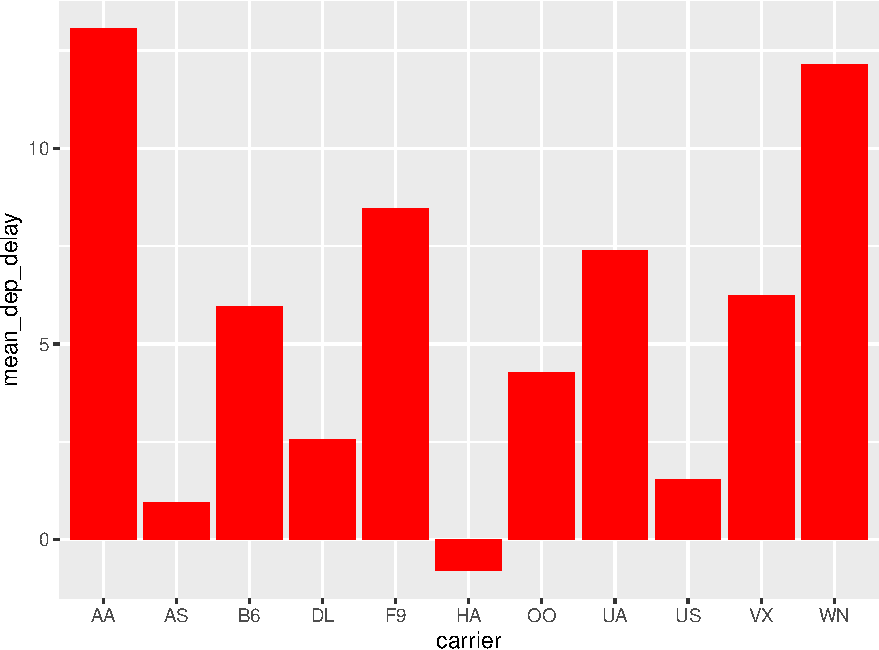
\includegraphics{thesis_files/figure-latex/delaysboxplot-1.pdf}
\caption{\label{fig:delaysboxplot}Mean Delays by Airline}
\end{figure}
Here is a reference to this image: Figure \ref{fig:delaysboxplot}.

A table linking these carrier codes to airline names is available at \url{https://github.com/ismayc/pnwflights14/blob/master/data/airlines.csv}.

\clearpage

Next, we will explore the use of the \texttt{out.extra} chunk option, which can be used to shrink or expand an image loaded from a file by specifying \texttt{"scale=\ "}. Here we use the mathematical graph stored in the ``subdivision.pdf'' file.
\begin{figure}
\includegraphics[scale=0.75]{figure/subdivision} \caption{Subdiv. graph}\label{fig:subd}
\end{figure}
Here is a reference to this image: Figure \ref{fig:subd}. Note that \texttt{echo=FALSE} is specified so that the \textbf{R} code is hidden in the document.

\textbf{More Figure Stuff}

Lastly, we will explore how to rotate and enlarge figures using the \texttt{out.extra} chunk option. (Currently this only works in the PDF version of the book.)
\begin{figure}
\includegraphics[angle=180, scale=1.1]{figure/subdivision} \caption{A Larger Figure, Flipped Upside Down}\label{fig:subd2}
\end{figure}
As another example, here is a reference: Figure \ref{fig:subd2}.

\hypertarget{footnotes-and-endnotes}{%
\section{Footnotes and Endnotes}\label{footnotes-and-endnotes}}

You might want to footnote something.\footnote{footnote text} The footnote will be in a smaller font and placed appropriately. Endnotes work in much the same way.

\hypertarget{cross-referencing-chapters-and-sections}{%
\section{Cross-referencing chapters and sections}\label{cross-referencing-chapters-and-sections}}

The \href{https://bookdown.org/yihui/bookdown/cross-references.html}{bookdown documentation} is an excellent source for learning how to cross-reference in a bookdown project such as a huskydown document. Here we only cover the most common uses for a typical thesis. If you want something more complex or fancy, please refer to the bookdown documentation and seek help from the developers of that package.

By default, all of your chapter and section headers will get an auto-generated ID label For example, e.g., \texttt{\#\ Chapter\ 1} will have an auto-generated ID \texttt{chapter-1}. Note that the ID label is all lower case, and has no spaces. If you have any kind of punctuation in your header, such as a colon (:), it will not appear in the ID label. Then in your text you can reference chapter one in your Rmd file like this: `as discussed in Chapter \texttt{\textbackslash{}@ref(chapter-1)},' which will print as `as discussed in Chapter 1'

We strongly recommend that you to manually assign ID labels to your chapter header to make it easy to cross-reference. For example, at the top of the Rmd file for this chapter, you can see:

\texttt{\#\ Tables,\ Graphics,\ References,\ and\ Labels\ \{\#ref-labels\}}

The \texttt{\{\#ref-labels\}} part of this header is the ID label. It doesn't show in the output, but is there for us to use for easy cross-referencing, because it can be short, and we don't need to change it elsewhere our document when we update the chapter header. We can use this custom ID label in our Rmd document like this: `as discussed in Chapter \texttt{\textbackslash{}@ref(ref-labels)},' which will print as `as discussed in Chapter \ref{ref-labels}.' If you need to show custom text instead of the chapter number, you use this syntax in your Rmd document: \texttt{see\ {[}my\ chapter\ about\ labels{]}(\#ref-labels)\ for\ more\ details} which will appear as `see \protect\hyperlink{ref-labels}{my chapter about labels} for more details'

To cross-reference a specific section in the same chapter, we recommend adding a custom ID label to the section header, and using that to cross-reference. For example, earlier in this chapter we have a section on tables and in the Rmd file we see \texttt{\#\#\ Tables\ \{\#tables\}}. We can cross-reference that in the text like this `as discussed in the section on \texttt{{[}tables{]}(\#tables)}' which will appear as `as discussed in the above section on \protect\hyperlink{tables}{tables}'

To cross-reference a section in a different chapter we can use the ID label from that section directly. For example, we can write in our Rmd document \texttt{as\ discussed\ in\ the\ section\ on\ {[}R\ code\ chunks{]}(\#r-chunks)\ in\ Chapter\ \textbackslash{}@ref(rmd-basics)} which will appear as `as discussed in the section on \protect\hyperlink{r-chunks}{R code chunks} in Chapter \ref{rmd-basics}.'

If you prefer to cross-reference by the section number, we can use custom ID labels in our Rmd document. For example, to refer to a section in our first chapter, we can write in the Rmd document: \texttt{as\ discussed\ in\ section\ \textbackslash{}@ref(r-chunks)\ in\ Chapter\ \textbackslash{}@ref(rmd-basics)}. This will appear with section and chapter numbers like so: as `as discussed in section \ref{r-chunks} in Chapter \ref{rmd-basics}.'

\hypertarget{bibliographies}{%
\section{Bibliographies}\label{bibliographies}}

Of course you will need to cite things, and you will probably accumulate an armful of sources. There are a variety of tools available for creating a bibliography database (stored with the .bib extension). In addition to BibTeX suggested below, you may want to consider using the free and easy-to-use tool called Zotero. Some Zotero documentation is at \url{http://libguides.reed.edu/citation/zotero}. In addition, a tutorial is available from Middlebury College at \url{http://sites.middlebury.edu/zoteromiddlebury/}.

\emph{R Markdown} uses \emph{pandoc} (\url{http://pandoc.org/}) to build its bibliographies. One nice caveat of this is that you won't have to do a second compile to load in references as standard LaTeX requires. To cite references in your thesis (after creating your bibliography database), place the reference name inside square brackets and precede it by the ``at'' symbol. For example, here's a reference to a book about worrying: (\protect\hyperlink{ref-Molina1994}{\textbf{Molina1994?}}). This \texttt{Molina1994} entry appears in a file called \texttt{thesis.bib} in the \texttt{bib} folder. This bibliography database file was created by a program called BibTeX. You can call this file something else if you like (look at the YAML header in the main .Rmd file) and, by default, is to placed in the \texttt{bib} folder.

For more information about BibTeX and bibliographies, see (\url{http://web.reed.edu/cis/help/latex/index.html})\footnote{(\protect\hyperlink{ref-reedweb2007}{\textbf{reedweb2007?}})}. There are three pages on this topic: \emph{bibtex} (which talks about using BibTeX, at \url{http://web.reed.edu/cis/help/latex/bibtex.html}), \emph{bibtexstyles} (about how to find and use the bibliography style that best suits your needs, at \url{http://web.reed.edu/cis/help/latex/bibtexstyles.html}) and \emph{bibman} (which covers how to make and maintain a bibliography by hand, without BibTeX, at \url{http://web.reed.edu/cis/help/latex/bibman.html}). The last page will not be useful unless you have only a few sources.

If you look at the YAML header at the top of the main .Rmd file you can see that we can specify the style of the bibliography by referencing the appropriate csl file. You can download a variety of different style files at \url{https://www.zotero.org/styles}. Make sure to download the file into the csl folder.

\textbf{Tips for Bibliographies}
\begin{itemize}
\tightlist
\item
  Like with thesis formatting, the sooner you start compiling your bibliography for something as large as thesis, the better.
\item
  The cite key (a citation's label) needs to be unique from the other entries.
\item
  When you have more than one author or editor, you need to separate each author's name by the word ``and'' e.g.~\texttt{Author\ =\ \{Noble,\ Sam\ and\ Youngberg,\ Jessica\},}.
\item
  Bibliographies made using BibTeX (whether manually or using a manager) accept LaTeX markup, so you can italicize and add symbols as necessary.
\item
  To force capitalization in an article title or where all lowercase is generally used, bracket the capital letter in curly braces.
\end{itemize}
\hypertarget{anything-else}{%
\section{Anything else?}\label{anything-else}}

If you'd like to see examples of other things in this template, please \href{https://github.com/benmarwick/huskydown/issues/new}{contact us} (email \href{mailto:bmarwick@uw.edu}{\nolinkurl{bmarwick@uw.edu}}) with your suggestions. We love to see people using \emph{R Markdown} for their theses, and are happy to help.

\hypertarget{recent-divergent-changes-in-alaskan-pinniped-trophic-position-detected-using-compound-specific-stable-isotope-analysis}{%
\chapter{Recent divergent changes in Alaskan pinniped trophic position detected using compound-specific stable isotope analysis}\label{recent-divergent-changes-in-alaskan-pinniped-trophic-position-detected-using-compound-specific-stable-isotope-analysis}}

\#\#Abstract

Over the past century Alaskan pinnipeds have experienced dramatic changes in abundance, but these changes have been highly variable across species and region. In recent decades, changes in atmospheric forcing and sea surface temperature have been particularly pronounced in the Gulf of Alaska and eastern Bering Sea, impacting the food webs in which Alaskan pinnipeds forage. We used compound-specific stable isotope analysis of nitrogen in amino acids to estimate historic and modern trophic position of harbor seals and Steller sea lions in the Gulf of Alaska and Bristol Bay. We applied a Bayesian hierarchical framework to determine whether shared trends through time exist across pinnipeds (classified by species and region) on decadal scales. Model results identified both shared trends through time and classification-specific decadal changes in pinniped trophic position. The largest change in trophic position occurred in the 2000s and 2010s and was observed in both Steller sea lions and harbor seals in the Gulf of Alaska, but not harbor seals in Bristol Bay or Iliamna Lake. Divergent trophic position patterns in the 2000s were identified in the western stock of Steller sea lions, which increased in trophic position, and sympatric harbor seals in the northern Gulf of Alaska, which decreased in trophic position. Our results indicate that these species have begun exploiting distinct trophic niches or experiencing unique food web conditions in recent decades in the Gulf of Alaska, likely in response to recent climate-induced ecological change in the region.

\#\#Introduction
Over the past century, pinniped populations in the northeast Pacific Ocean have experienced changes in adult and pup abundances (\protect\hyperlink{ref-Muto2020}{\textbf{Muto2020?}}). Understanding specific drivers of these population trends is important for management, as multiple stocks have been listed as threatened or endangered over the past two decades (\protect\hyperlink{ref-Muto2020}{\textbf{Muto2020?}}). The observed population dynamics have also corresponded with shifts in both the physical and ecological marine environment, which frequently occur simultaneously. As a result, disentangling drivers of population trends is complex, as multiple factors (environmental conditions, prey availability, anthropogenic disturbances) can change in tandem and potentially act synergistically on pinniped populations.

Data on long-term trends in trophic position across regions, species, and populations is one potential way to assess how food web changes have impacted pinnipeds in Alaska. This approach can identify how broad shifts in foraging ecology correspond to changes in abundance and population dynamics. More specifically, examining trophic position during periods of declining versus increasing predator abundance can provide insight into whether foraging behavior and prey availability are important drivers of population dynamics. In this study, we aim to identify whether common temporal trends in trophic ecology exist across harbor seals (\emph{Phoca vitulina}) and Steller sea lions (\emph{Eumetopias jubatus}) and their locations by deriving 70-years of trophic position data from compound-specific stable isotope analysis (CSIA) of museum specimens.

Following climatic changes in the 1970s that altered ocean currents and sea surface temperature (\protect\hyperlink{ref-Hare2000}{\textbf{Hare2000?}}), most Gulf of Alaska and Bering Sea pinniped populations experienced declines that persisted through the 1990s (\protect\hyperlink{ref-Muto2020}{\textbf{Muto2020?}}). However, these responses differed across populations and species. For example, the western stock of Steller sea lions (located west of 144°W) decreased from approximately 240,000 animals in the late 1970s to 50,000 in 2000 (\protect\hyperlink{ref-Burkanov2005}{\textbf{Burkanov2005?}}). Similarly, harbor seal populations in Prince William Sound and Glacier Bay declined by approximately 60\% between the 1980s and 2000 (\protect\hyperlink{ref-Frost1999}{\textbf{Frost1999?}}; \protect\hyperlink{ref-Womble2010}{\textbf{Womble2010?}}). In contrast, the eastern stock of Steller sea lions (located east of 144°W) increased by 3-4\% per year over the same time period (Figure 2) (\protect\hyperlink{ref-Muto2020}{\textbf{Muto2020?}}; \protect\hyperlink{ref-Pitcher2007}{\textbf{Pitcher2007?}}). More recently, atmospheric circulation anomalies in the northeast Pacific Ocean have resulted in unprecedently warm sea surface temperatures during the past decade (\protect\hyperlink{ref-Walsh2018}{\textbf{Walsh2018?}}) and this environmental shift has altered fish abundances (\protect\hyperlink{ref-Litzow2020}{Litzow et al., 2020}; \protect\hyperlink{ref-Bond2015}{\textbf{Bond2015?}}). For example, the unprecedented marine heatwave that occurred in 2014 - 2016 triggered dramatic ecosystem change, including a 71\% decline in Pacific cod in the Gulf of Alaska (\protect\hyperlink{ref-Barbeaux2020}{\textbf{Barbeaux2020?}}). Declines in phytoplankton biomass, forage fish abundance, and changes in community structure as a whole were also observed (\protect\hyperlink{ref-Suryan2021}{\textbf{Suryan2021?}}). During this recent period of environmental change, many pinniped populations have experienced increases or stabilization of population abundance (\protect\hyperlink{ref-Muto2020}{\textbf{Muto2020?}}) (Figure 2), although declines in some Gulf of Alaska Steller sea lion populations were observed following the marine heat wave (\protect\hyperlink{ref-Suryan2021}{\textbf{Suryan2021?}}).

These variable changes in Alaskan pinniped populations over the past 50 years cannot be attributed to a single cause, as multiple environmental, anthropogenic, and ecological factors have changed simultaneously. For example, the rapid decline of the western stock of Steller sea lions between the 1970s and 1990s has been attributed to myriad factors, including change to the physical environment, competition with fisheries for common prey, predation, disease, and human-caused mortality (\protect\hyperlink{ref-Atkinson2008}{\textbf{Atkinson2008?}}). Glacier Bay harbor seal populations have primarily, but not exclusively, been impacted by the decline of sea ice, which provides a majority of their haulout sites (\protect\hyperlink{ref-Womble2010}{\textbf{Womble2010?}}). Population declines have also been associated with increased numbers of tour vessels, particularly in glacier fjords that provide important nursing and whelping habitat (\protect\hyperlink{ref-Jansen2015}{\textbf{Jansen2015?}}; \protect\hyperlink{ref-Matthews2016}{\textbf{Matthews2016?}}). The differences in pinniped population trends across the Gulf of Alaska and Bering Sea suggest varied environmental and ecological drivers underlying these dynamics. Interestingly, harbor seals and Steller sea lions that occur in the same geographic region (sympatric) have experienced different population trends over similar time period (Figure 2). Identifying trophic position trends through time that are shared, compared to changes that only impact a specific species or region, can elucidate how widescale ecological forcing versus localized change influence top predators and potentially explain variable population abundance trends.

Both harbor seals and Steller sea lions exhibit generalist, piscivorous foraging strategies, although differences in foraging range, body size, and diet exist. Adult harbor seals have high site fidelity, opportunistically forage 5 - 10 km from haulout sites and at depths \textless{} 200 m (\protect\hyperlink{ref-Lance2012}{Lance, Chang, Jeffries, Pearson, \& Acevedo-Gutiérrez, 2012}; \protect\hyperlink{ref-Lowry2001}{\textbf{Lowry2001?}}), and weigh up to 300 pounds. Steller sea lions are central place foragers known to migrate to prey aggregations on the continental shelf and oceanographic boundary zones (\protect\hyperlink{ref-Sinclair2002}{\textbf{Sinclair2002?}}; \protect\hyperlink{ref-Womble2006}{\textbf{Womble2006?}}). Foraging trips can last 1-3 days (\protect\hyperlink{ref-Maniscalco2006}{\textbf{Maniscalco2006?}}) with average distances of 133 km for adult females (\protect\hyperlink{ref-Merrick1997}{\textbf{Merrick1997?}}), although foraging trips are shorter in the breeding season (\protect\hyperlink{ref-Maniscalco2006}{\textbf{Maniscalco2006?}}). Adult females can weigh up to 800 pounds whereas adult males can exceed 2,500 pounds, indicating a higher energetic demand compared to harbor seals. Diet studies of Steller sea lions and harbor seals are spatially and temporally limited, and primarily utilize scat samples. In the Gulf of Alaska, gadids, cephalopods, and forage fishes are prevalent in both harbor seal and Steller sea lion diet (\protect\hyperlink{ref-Sinclair2002}{\textbf{Sinclair2002?}}; \protect\hyperlink{ref-Geiger2013}{\textbf{Geiger2013?}}), whereas salmonids are also important for harbors seals in Bristol Bay and Iliamna lake (\protect\hyperlink{ref-Hauser2008}{\textbf{Hauser2008?}}).

Stable isotopes have been used to reconstruct historical differences in diet and trophic position in Alaskan pinnipeds (\protect\hyperlink{ref-Hobson1997}{\textbf{Hobson1997?}}; \protect\hyperlink{ref-Hirons2001}{\textbf{Hirons2001?}}; \protect\hyperlink{ref-Brennan2019}{\textbf{Brennan2019?}}). These previous studies utilized bulk stable isotope analysis exclusively and were therefore limited in their inferential strength. Differences in the bulk \textsuperscript{15}N/\textsuperscript{14}N of consumer tissues can indicate either a trophic level change of the consumer or a change in nitrogen resources at the base of the food web. The specific cause of the isotopic variation cannot be ascertained from consumer bulk stable isotope values unless the data are paired with temporal information on \textsuperscript{15}N/\textsuperscript{14}N in primary producers. Lack of consistent, concurrent sampling of nitrogen stable isotope composition of primary producers therefore presents a challenge for previous long-term studies of the trophic dynamics of consumers from bulk stable isotope data. CSIA data address this challenge, as amino acids exhibit two distinct patterns in isotopic enrichment: trophic amino acids (i.e., glutamic acid, alanine, proline) become enriched in \textsuperscript{15}N with each trophic transfer and source amino acids (i.e., phenylalanine) show minimal change and thus are reflective of the base of the food web (\protect\hyperlink{ref-Chikaraishi2009}{Yoshito Chikaraishi et al., 2009}; \protect\hyperlink{ref-McClelland2002}{McClelland \& Montoya, 2002}; \protect\hyperlink{ref-Ohkouchi2017}{Ohkouchi et al., 2017}). With the ability to internally correct for expected changes in \textsuperscript{15}N/\textsuperscript{14}N at the base of the food web (\protect\hyperlink{ref-Feddern2021}{\textbf{Feddern2021?}}; \protect\hyperlink{ref-McMahon2021}{\textbf{McMahon2021?}}), CSIA allows for a more robust retrospective analysis of consumer trophic dynamics on decadal and century scales.

The objective of this work is to describe and compare changes in trophic ecology for Alaskan pinnipeds throughout the past century and investigate trophic position differences for sympatric populations. We apply hierarchical Bayesian analyses to 70 years of trophic position data derived from CSIA from pinnipeds (harbor seal and Steller sea lion) in the Gulf of Alaska, Bristol Bay, and a small population of freshwater harbor seals in Iliamna Lake, Alaska which is adjacent to Bristol Bay. We build on previous research examining pinniped nitrogen stable isotope composition (\protect\hyperlink{ref-Misarti2009}{Misarti, Finney, Maschner, \& Wooller, 2009}; \protect\hyperlink{ref-Hobson1997}{\textbf{Hobson1997?}}; \protect\hyperlink{ref-Hirons2001}{\textbf{Hirons2001?}}; \protect\hyperlink{ref-Brennan2019}{\textbf{Brennan2019?}}) by adding two decades of data to the record (2000s and 2010s) and incorporating a broad spatial scope (Bristol Bay, Iliamna Lake, Gulf of Alaska). Additionally, by analyzing nitrogen stable isotopes derived from amino acids, we were able to control for known changes in nitrogen resources and phytoplankton composition at the base of the food web that can confound trophic position interpretations from bulk stable isotope data collected over decadal scales (\protect\hyperlink{ref-Feddern2021}{\textbf{Feddern2021?}}). Furthermore, by comparing trophic position dynamics across species and region through time, regional and location-specific ecological responses to a changing ecosystem can be identified.

\#\#Methods

\#\#\#Sample collection and analysis

Samples were obtained using methods described in (\protect\hyperlink{ref-Feddern2021}{\textbf{Feddern2021?}}). Briefly, harbor seal and Steller sea lion bones were sampled from specimens curated at the University of Alaska Museum of the North (Supplementary Information Table S1). Specimens were treated by maceration in warm water and soaked in a dilute ammonia solution then stored in acid free boxes. Adult specimens were sampled exclusively to avoid dietary differences between adults and juveniles. Specimens were classified based on species and region. We prioritized long-term temporal coverage in four regional classifications of harbor seals (Iliamna Lake, southeast Gulf of Alaska, northern Gulf of Alaska, eastern Bering Sea) and two regional classifications of Steller sea lions (eastern and western stocks) for a total of 6 species x region classifications. Specimens were extremely limited for the eastern Steller sea lion stock (n = 2) and Iliamna Lake harbor seas (n = 3). We also prioritized specimens with sex and age identifications, but these data were not available for some specimens. A total of 106 harbor seal and 21 Steller sea lion specimens were sampled representing the 1950s to 2010s (Figure 1).

Steller sea lions were classified according to the National Oceanic and Atmospheric Administration's (NOAA) distinct population segments, where Steller sea lions east of 144°W are considered the eastern stock and west of 144°W are considered the western stock (Figure 1). NOAA has identified twelve stocks of harbor seals in Alaska and, due to limitations of archived specimens, harbor seals were not able to be classified according to NOAA stocks. Instead, they were classified based on their range relative to the Steller sea lion stocks and utilization of marine versus freshwater habitats. Harbor seals that were west of 144°W, which included samples from the Prince William Sound and Cook Inlet/Shelikof Strait stocks (Figure 1), were classified as northern Gulf of Alaska harbor seals. Harbor seals that were located east of 144°W, which included samples from the Glacier Bay/Icy Strait, Sitka/Chatham Strait, Lynn Canal/Stephens Passage, Dixon/Capes Decisions, and Clarence Strait stocks (Figure 1), were classified as southeast Gulf of Alaska harbor seals. The Bristol Bay harbor seal stock was divided into two classifications, Bristol Bay referring to marine harbor seals, and Iliamna Lake referring to freshwater harbor seals (Figure 1). This allowed for comparison of three pairs of geographically overlapping classifications: western stock of Steller sea lions and northern Gulf of Alaska harbors seals, eastern stock of Steller sea lions and southeast Gulf of Alaska harbor seals, and Bristol Bay and Iliamna Lake harbor seals.

\#\#\#Trophic position calculation

Bone collagen within the samples was decalcified, acid hydrolyzed, derivatized and analyzed for compound-specific stable isotope analysis (CSIA) of nitrogen (\(\delta^{15}N\)) for 12 individual amino acids following the protocol described in (\protect\hyperlink{ref-Feddern2021}{\textbf{Feddern2021?}}). \(\delta^{15}N\) was measured as:
\begin{equation} 
  \delta^{15}N ( \textperthousand vs. air) =   
  [(\frac{^{15}N/^{14}N_{Sample}}{^{15}N/^{14}N_{Air}} -1)*1000]
  \label{eq:deltN2}
\end{equation}
Collagen samples were measured in triplicate with a laboratory standard containing a 12 amino acid mixture of known isotopic composition. Full analytical details are described in Appendix S1.

Trophic position was calculated using a harbor seal-specific trophic discrimination factor (difference in \textsuperscript{15}N/\textsuperscript{14}N between trophic and source amino acids in consumers for a trophic transfer; \protect\hyperlink{ref-Germain2013}{Germain, Koch, Harvey, \& McCarthy} (\protect\hyperlink{ref-Germain2013}{2013})). This approach assumed trophic discrimination factors (TDF) derived from controlled feeding studies of harbor seals were similar to Steller sea lions. Applying a ``multi-TDF'' approach that combines both average and taxa-specific TDF can improve trophic position estimates in marine predators including pinnipeds (\protect\hyperlink{ref-Germain2013}{Germain, Koch, Harvey, \& McCarthy, 2013}; \protect\hyperlink{ref-McMahon2019}{McMahon et al., 2019}). The following equation was used to determine the trophic position of each sampled individual:
\begin{equation} 
Trophic Position =   
  \frac{\delta^{15}N_i - \delta^{15}N_o - TDF_{(i-o),j} - \overline{\beta}_{(i-o)}}{\overline{TDF}_{(i-o)}}+2
  \label{eq:TP}
\end{equation}
where, \(\delta^{15}N_i\) is the measured stable isotope composition of a trophic amino acid i in a sample and \(\delta^{15}N_o\) is the stable isotope composition of a source amino acid o in a sample. \(\overline{TDF}_{(i-o)}\) is the mean difference between given trophic amino acid \emph{i} and source amino acid \emph{o} across all consumers described in (\protect\hyperlink{ref-Nielsen2015}{\textbf{Nielsen2015?}}). \(TDF_{(i-o), j}\) is the trophic discrimination factor between trophic amino acid \emph{i} and source amino acid \emph{o} from a controlled feeding study of a specific consumer \emph{j}; here we use harbor seals from \protect\hyperlink{ref-Germain2013}{Germain, Koch, Harvey, \& McCarthy} (\protect\hyperlink{ref-Germain2013}{2013}) (Table 1). \(\overline\beta_{(i-o)}\) is the mean difference in \(\delta^{15}N\) across aquatic phytoplankton between a specific trophic amino acid \emph{i} and source amino acid \emph{o} {[}(\protect\hyperlink{ref-Nielsen2015}{\textbf{Nielsen2015?}}); Table 1{]}. (\protect\hyperlink{ref-Nielsen2015}{\textbf{Nielsen2015?}}) also determined using multiple amino acids to estimate trophic position improves precision. Therefore, we used multiple trophic amino acids \emph{i} (alanine, glutamic acid, aspartic acid and proline) and one source amino acid \emph{o} (phenyalanine) to calculate trophic position (Table 1). These amino acids were chosen based on their prevalence in previous studies to derive parameters for equation 2, and their concentrations in bone collagen (see Appendix S1).

\#\#\#Model framework
Sex was considered as a predictor for trophic position, however, sex metadata were not available for all specimens. In order to evaluate difference in trophic position by sex, we fit linear statistical models to each individual trophic amino acid, by classification (species x region). These models took the following form:
\begin{equation} 
y_i = \alpha + \boldsymbol\beta x_i + \epsilon_i, \epsilon \sim N(0,\sigma)
  \label{eq:linsex}
\end{equation}
where, \(y_i\) is trophic position for an individual amino acid and \(\boldsymbol\beta\) is a vector of coefficients for the predictor, in this case sex, and \(\epsilon\) are residual errors assumed to be normally distributed with mean 0 and standard deviation \(\sigma\). There was not sufficient metadata for the eastern stock Steller sea lion population or the Iliamna Lake population and these two classifications were omitted from this analysis.

A Bayesian hierarchical mixed effects model was used to identify decadal change across pinniped classifications (species x region), and the degree to which these changes were shared by testing the effects of classification, decade, and a classification-decade interaction as either population-level (fixed) or group-level (random) effects (see candidate models in Table 2). Hierarchical models share information across `groups' to identify common responses, which refers to both decade and classification in this study. The interaction term allows for increased flexibility, letting each classification have slight departures from the group-level means. The mean and variance of pinniped trophic position for each region-species classification and decade were estimated using a generalized linear Bayesian hierarchical model with decade, population, and trophic amino acid as predictors:
\begin{equation} 
y_i = \boldsymbol\alpha + \boldsymbol\beta x_i + \epsilon_i, \epsilon \sim N(0,\sigma_y)
  \label{eq:linsex}
\end{equation}
\begin{equation} 
\boldsymbol\alpha_{k=1:k} \sim N(\mu_{\alpha,k},\sigma_{\alpha,k})
  \label{eq:linsex}
\end{equation}
where, for data point \emph{i}, \(\boldsymbol\beta\) is a vector of coefficients for the unpooled predictors (fixed effects, Table 2) and \(\boldsymbol\alpha\) is a vector of coefficients for the partially pooled group-level predictors (random effects, Table 2) for group \emph{k} (amino acid, decade or classification). At minimum, the \(\boldsymbol\alpha\) included a random term for the amino acid corresponding to data point \emph{i}, and depending on the model included up to a total of 4 random effects (also effects of decade, classification, and their interaction, Model 6 in Table 2). For each random effect included, \(\mu_{α,k}\) and \(\sigma_{α,k}\) are hyperparameters representing the mean and standard deviation of group-level effects on trophic position, for random effect \emph{k}. For models with more than one random effect, we assumed the deviations to be independent and uncorrelated. We considered models that included decade, classification, and the interaction between decade and classification either as fixed or random effects (e.g.~Model 4 v Model 6, Table 2), but did not consider models that included both as fixed and random (Table 2). Parameter estimates were obtained using the brms package ((\protect\hyperlink{ref-Burkner2017}{\textbf{Burkner2017?}}), version 2.14.4) in R (R Core Development Team 2021, version 3.6.2), which implements a Hamiltonian Monte Carlo sampler and its extension no-U-turn sampler (\protect\hyperlink{ref-Hoffman2014}{\textbf{Hoffman2014?}}) through Stan (Stan Development Team 2020). Minimally informative priors were used for random effects (normal distributions with a mean of 0 and variance of 10) and fixed effects (Student's t-distribution with a mean of 0, standard deviation of 2.5 and 3 degrees of freedom). Trophic amino acid was included as a random effect for all models (Table 2). Selection of the best models (Table 2) given the data was based on approximate leave-one-out cross-validation (LOOIC) using the loo package ((\protect\hyperlink{ref-Veharti2017}{\textbf{Veharti2017?}}), version 2.4.1).

\#\#Results
We found no differences between the average male and female pinniped trophic position over the 50-year study period (Figure 3) for the four tested species-region classifications. This finding was consistent for all trophic amino acids-source amino acid pairs (Figure 3). Based on glutamic acid trophic position estimates, both western stock Steller sea lions (2.6 ± 0.5; mean ± sd) and eastern stock Steller sea lions (2.7 ± 0.16) had similar trophic positions. Harbor seals in the Gulf of Alaska foraged higher in the food web than their Steller sea lion counterparts (Figure 3). Harbor seals in the southeast region had a higher trophic position on average than any other pinniped in this study (3.5 ± 0.3) but were similar to harbor seals in the northern region (3.3 ± 0.5). Bristol Bay (3.1 ± 0.4) and Iliamna lake (3.0 ± 0.3) harbor seals had a lower trophic position than their Gulf of Alaska counterparts on average (Figure 3).

\#\#\#Common trends in Alaskan pinniped trophic position

The best performing model (Table 2, model 6) of pinniped trophic position included both species-region classification and decade as random effects (shared trends) along with an interaction between population and decade (Table 2). Based on the support for decade and classification to be included as group-level effects, these data support consistent differences between classifications over time, as well as differences between trophic position for all classifications. The supported interaction between population and decade (Table 2) indicates distinct decadal changes in trophic position for species-region classifications exist. The model that included decade, classification, and the interaction between decade and classification as fixed effects (model 4) was also supported based on the models LOOIC (Table 2). Therefore, the inclusion of the interaction term was more important for improving model performance than inclusion of decade and classification as fixed versus random effects.

There were consistent differences in trophic position that varied by species and ocean basin for the model with the most support. Harbor seals in the Gulf of Alaska had higher trophic position than their Steller sea lion counterparts. The mean difference of the posterior distributions indicated southeast Gulf of Alaska harbor seals have historically fed at 0.32 {[}-0.01, 0.61{]} (highest density 80\% credible interval) trophic levels higher than sympatric eastern stock Steller sea lions (Figure 4). Similarly, the mean difference of posterior distributions showed northern Gulf of Alaska harbor seals fed 0.28 {[}-0.03, 0.50{]} trophic levels higher than the sympatric western stock Steller sea lions. Within the Gulf of Alaska, the posterior distributions for trophic position overlapped 39\% between harbor seals and Steller sea lions in both the eastern and western regions (Figure 4). Iliamna Lake harbor seals have historically fed at a lower trophic level (mean posterior difference 0.16 {[}-0.11, 0.41{]}) than harbor seals in Bristol Bay, but these two classifications have 66\% overlap of the group-level posterior distributions for trophic position (Figure 4). The 80\% credible intervals included 0 for most region-species classifications thus the posterior probabilities support marginal evidence for consistent differences in trophic position between classifications. Regardless, the differences in posterior means were large, although the distributions were wide.

There were no consistent decadal differences in trophic position across the region-species classification (Figure 5). Pinniped trophic position in the 2000s was slightly higher for all classifications (mean posterior difference 0.03 {[}-0.09, 0.16{]}) on average compared to 1990 and the posterior distributions for 1990 and 2000 had an 85\% overlap (Figure 5). Similarly, posterior distributions in between 2000 and 2010 had a mean difference of -0.1 {[}-0.27, 0.08{]} with a 65\% overlap (Figure 4). Overall, decadal differences in pinniped trophic position through time were smaller than the region-species classification effects and were likely ecologically inconsequential.

\#\#\#Spatial and temporal differences in pinniped trophic structure

Distinct decadal changes in trophic position were observed for each species-region classification and varied more than the shared decadal changes (Figure 6) as indicated by the decade-classification interaction. Most, but not all, pinniped classifications experienced substantial trophic level change in 2000 or 2010 but the magnitude and direction of this change varied by region-species classification based on the combined effects of decade, classification, and the decade-classification interaction (Figure 6). The recent decadal change in trophic position was most prominent for the western stock of Steller sea lions which had a mean trophic level decrease of 0.43 {[}-0.25, -0.60{]} from 1990 to 2000 (a percent decrease of 0.15) with only a 21\% overlap between the posterior distributions (Figure 6E). This decline in trophic position remained in the 2010s. A similar decline was observed in the southeast Gulf of Alaska harbor seals. This population experienced relatively stable trophic position from 1960-1990, which then declined on average by 0.31 {[}-0.19, -0.45{]} trophic levels in 2000 (33\% posterior overlap) (Figure 6C). In contrast, harbor seals in the northern Gulf of Alaska had variable trophic position across decades and had the highest trophic position in 2000 in contrast to their southeast Gulf of Alaska harbor seals and Steller sea lion counterparts (Figure 6B). Data were only available for 2000 and 2010 for the eastern stock Steller sea lions, and trophic position was similar for this population during both of these decades (Figure 6F). Both Bristol Bay and Iliamna Lake harbor seals had relatively stable trophic position from 1950s until 2010s (Figure 6A \& B). Bristol Bay harbor seals experienced their lowest trophic level in the 1990s with a 0.24 {[}-0.54, 0.00{]} trophic level decrease compared to the 1970s and 2000s, but the posterior distribution still overlapped 54\% with other decades (Figure 6A).

\#\#Discussion

Over the past 70 years, Alaskan pinnipeds have exhibited both common and distinct differences in trophic position across region-species classification on decadal scales (Table 2). While potential drivers of change in trophic position were not tested in this study due to data limitations, our results support a combination of local-scale (i.e., vessel traffic, reduction of glacial ice, local foraging) and regional-scale (i.e., environmental condition, basin-wide prey abundance) changes may be influencing pinniped trophic ecology. Furthermore, the largest decadal changes in pinniped trophic position were distinct for each region-species classification and were most apparent during the most recent two decades (2000s and 2010s). These patterns are more pronounced in the Gulf of Alaska compared to Bristol Bay (Figures 5 \& 6).

\#\#\#Regional and species trends in harbor seal trophic position

Both Steller sea lions and harbor seals exhibit generalist foraging patterns (\protect\hyperlink{ref-Lance2012}{Lance, Chang, Jeffries, Pearson, \& Acevedo-Gutiérrez, 2012}; \protect\hyperlink{ref-Geiger2013}{\textbf{Geiger2013?}}). Diets of Alaskan pinnipeds consist of similar prey species but vary between species, population, and local availability of prey (\protect\hyperlink{ref-Iverson1997}{\textbf{Iverson1997?}}; \protect\hyperlink{ref-Hirons2001}{\textbf{Hirons2001?}}). Bulk stable isotope studies in the Gulf of Alaska have shown that Steller sea lions feed lower in the food web compared to harbor seals (\protect\hyperlink{ref-Iverson1997}{\textbf{Iverson1997?}}). Our CSIA analysis confirms the interpretation of these previous studies that isotopic differences can be attributed to trophic position changes and not isotopic shift of basal phytoplankton resources. Both western and eastern stock Steller sea lions have lower trophic position compared to sympatric harbor seal populations but have similar trophic position compared to other populations such as Iliamna Lake. However, despite known differences in both diet (\protect\hyperlink{ref-Sinclair2002}{\textbf{Sinclair2002?}}; \protect\hyperlink{ref-Geiger2013}{\textbf{Geiger2013?}}) and nearshore versus offshore foraging (\protect\hyperlink{ref-Merrick1997}{\textbf{Merrick1997?}}; \protect\hyperlink{ref-Lowry2001}{\textbf{Lowry2001?}}) between the two species, our results also show historical overlap in trophic position, indicating potential trophic redundancy between harbor seals and Steller sea lions in the Gulf of Alaska.

Harbor seals in Bristol Bay and Iliamna Lake are managed as a single population (\protect\hyperlink{ref-Muto2020}{\textbf{Muto2020?}}) despite lack of evidence of migration by the freshwater population and utilization of different resources (\protect\hyperlink{ref-Brennan2019}{\textbf{Brennan2019?}}). A previous study of strontium and carbon stable isotopes showed Iliamna Lake harbor seals utilize freshwater-derived resources (resident lake fishes), particularly early in life, and exhibit an ontogenetic shift to more marine resources (returning sockeye salmon) later in life (\protect\hyperlink{ref-Brennan2019}{\textbf{Brennan2019?}}). Based on CSIA nitrogen data, Iliamna Lake harbor seals also forage lower in the food web compared to Bristol Bay harbor seals. In addition, both classifications exhibited trophic stability, with the Bristol Bay harbor seals only experiencing a trophic shift in the 1990s relative to the 1960s and 1970s. This coincided with the lowest sockeye salmon returns to Iliamna Lake on record (\protect\hyperlink{ref-Hilborn2003}{\textbf{Hilborn2003?}}). Interestingly, the decrease in trophic position in the 1990s occurred simultaneously with decreases in basin wide Bristol Bay harbor seal abundance in the late 1990s, which then stabilized and increased in the 2000s and 2010s (Figure 2). Data were not available for the freshwater harbor seals between 1990 and 2000 and thus it is unclear whether the freshwater population also experienced a trophic position change during the 1990s when sockeye salmon returns were low. While quantitative comparisons to salmon abundance were not made in this study, salmon population abundance and harbor seal trophic ecology and population trends are seemingly interrelated.

\#\#\#Recent trophic position changes in the Gulf of Alaska

Trophic position changes were observed in all pinniped classifications in the Gulf of Alaska during the past two decades, although the direction of these changes varied on more local scales. During the past two decades (2000-2020), harbor seals in the Gulf of Alaska have experienced stabilization of most monitored populations following long-term declines that persisted from the 1950s through the 1990s (Figure 2, (\protect\hyperlink{ref-Muto2020}{\textbf{Muto2020?}})). During this same time period, harbor seals in both southeast and northern Gulf of Alaska experienced a shift in trophic position that was particularly prominent in the 2000s compared to historic estimates of trophic position (Figure 6B \& C). It is possible that the observed trophic position shift may have contributed to the population stabilization of Gulf of Alaska harbor seals, either by an increase in prey availability or opportunistically foraging on a novel prey source. (\protect\hyperlink{ref-Gagne2018}{\textbf{Gagne2018?}}) observed similar trophic position declines in seabird populations, which were attributed to a shift in diet from fish to squid. A similar dietary shift could explain the observed trophic position shift in southeast Gulf of Alaska harbor seals and western stock Steller sea lions.

Recent regional change in the Gulf of Alaskan food webs has been well documented in other species and primarily attributed to bottom-up effects of climate (\protect\hyperlink{ref-Litzow2020}{Litzow et al., 2020}; \protect\hyperlink{ref-Barbeaux2020}{\textbf{Barbeaux2020?}}). These region-wide trends likely altered prey availability for pinniped populations in the Gulf of Alaska. How pinniped populations have adapted their foraging ecology, however, indicates regional and species trophic divergence, which could be attributed to either local-scale foraging adaptations or differences in prey availability. Pinniped groups that overlap in space (Figure 1) revealed divergent trends in trophic position between Steller sea lions and harbor seals in recent decades (Figure 6B \& E). For example, trophic position of northern Gulf of Alaska harbor seals increased in the 2000s while the western stock of Steller sea lions decreased. For western stock Steller sea lions, this shift also persisted into the 2010s (Figure 6E). Posterior distributions of western stock Steller sea lions and northern Gulf of Alaska harbor seals overlapped by 63\% in the 1950s but only overlapped by 3\% in the 2000s (Figure 6B \& E). The recent change in pinniped trophic position within the Gulf of Alaska coincided with population abundance stabilization, albeit at lower than historical abundance for most populations. This trophic divergence indicates there could be increased competition for resources between northern Gulf of Alaska harbor seals and western stock Steller sea lions resulting in diet adaptations. Similar comparisons were challenging to make for the eastern stock of Steller sea lions and southeast Gulf of Alaska harbor seals due to limitations in historical data for the former. However, trophic position in the 2000s showed a 38\% overlap (Figure 6C \& E) between the two species, indicating any trophic divergence between them may be less pronounced in this region, if existent.

The observed divergent trends indicate differences in how Alaskan pinnipeds are adapting to environmental and ecological changes. Trophic position changes from stable isotope data can be accounted for by: 1) prey switching between different species, 2) consuming different sizes of the same prey, or 3) consuming different quality prey. These changes can occur at the consumer level (pinnipeds) or lower in the food web and still be reflected in consumer stable isotope signature and thus trophic position. In recent decades, Pacific salmon and halibut in Alaska have both declined in size (\protect\hyperlink{ref-Holsman2019}{\textbf{Holsman2019?}}; \protect\hyperlink{ref-Oke2020}{\textbf{Oke2020?}}). These changes in size distributions of prey have been attributed to changes in marine mammal populations (Groskreutz et al.~2019) and likely contributed to the observed trophic position declines in western Steller sea lion and southeast Gulf of Alaska harbor seals. In contrast, consuming low-quality prey with lower protein content and greater amino acid imbalance between consumer and prey increases the amino acid trophic enrichment factor of nitrogen (\protect\hyperlink{ref-McMahon2015}{\textbf{McMahon2015?}}). If not accounted for in trophic position equations, this increase in trophic enrichment factor can result in erroneously high trophic position estimates. This may explain the observed increase in estimated trophic position in northern Gulf of Alaska harbor seals where this population may be consuming a greater proportion of lower quality prey (i.e., crustaceans, shrimp, cephalopods) in recent decades rather than feeding on prey species that are higher in the food web.

\#\#\#Considerations and limitations for CSIA analyses

The data in this study were limited in sample size primarily due to the availability of archived specimens. As a result, we were not able to discern between known fine scale differences in populations or annual trends. For example, harbor seals in the southeast Gulf of Alaska consist of 13 individual stocks. Due to limitations in the number of archived specimens, these stocks were pooled and analyzed as a single classification despite known differences in genetic structure (\protect\hyperlink{ref-Muto2020}{\textbf{Muto2020?}}). Given the observed broad range in trophic position of these generalist predators, it is unlikely that inclusion of finer spatial dynamics would have changed the supported model, although variation in temporal trends within a classification may have been identified. Similarly, data were only available for eastern stock Steller sea lions for 2000s and 2010s. As a result, no historical comparisons were possible and the conclusions about this population are tentative. Nonetheless, this dataset offers historic documentation of pinniped trophic position that can be updated with future samples or additional archived specimens.

Trophic position estimates in this study were low compared to known foraging strategies of these pinnipeds. For example, Steller sea lions eat primarily walleye pollock and Atka mackerel (\protect\hyperlink{ref-Hobson1997}{\textbf{Hobson1997?}}; \protect\hyperlink{ref-Trites2007}{\textbf{Trites2007?}}), which would indicate a trophic position of 3 or higher. Mean trophic position for Steller sea lions was closer to 2.7 in this study, which is lower than expected based on known foraging ecology. It is common for CSIA to underestimate trophic position of marine predators (\protect\hyperlink{ref-Germain2013}{Germain, Koch, Harvey, \& McCarthy, 2013}; \protect\hyperlink{ref-McMahon2019}{McMahon et al., 2019}) and the inclusion of multiple amino acid pairs and a multi-trophic enrichment factor framework did not fully resolve this issue. (\protect\hyperlink{ref-Nielsen2015}{\textbf{Nielsen2015?}}) found trophic position estimates can be highly sensitive to the applied \(\beta\) values in equation 2. In our trophic position calculation, we assumed a constant \(\beta\) represented by marine diatoms. However, \(\beta\) values differ by more than 11 per mille between seagrasses and diatoms (\protect\hyperlink{ref-VanderZanden2013}{\textbf{VanderZanden2013?}}) which has been attributed to differences between vascular and nonvascular plants (\protect\hyperlink{ref-Ramirez2021}{\textbf{Ramirez2021?}}). If vascular plants, such as seagrasses, contribute to the food web in addition to non-vascular algae, the applied β would be too high and would result in underestimation of trophic position of marine consumers (\protect\hyperlink{ref-Ramirez2021}{\textbf{Ramirez2021?}}). Even a 10\% contribution of vascular plant-derived nitrogen to the food web would result in an underestimation of 0.2 trophic position. It is likely that vascular plants at least partially contribute to the Alaskan food web, as seagrass beds provide essential habitat and food for many fish species and invertebrates. Consideration for variable \(\beta\) values may be helpful in resolving trophic position underestimation of future studies, especially in cases where consumer carbon stable isotope data is available and contributions of seagrasses to the food web are well documented.

\#\#\#Conclusions and Implications

Marine ecosystems in Alaska are experiencing unprecedented environmental change that has altered abundance and size distributions of many fish species consumed by pinnipeds (\protect\hyperlink{ref-Barbeaux2020}{\textbf{Barbeaux2020?}}; \protect\hyperlink{ref-Holsman2019}{\textbf{Holsman2019?}}; \protect\hyperlink{ref-Oke2020}{\textbf{Oke2020?}}; \protect\hyperlink{ref-Suryan2021}{\textbf{Suryan2021?}}). Heterogeneity in diet and foraging locations allow top predators to adjust to availability of resources by altering their foraging. Based on the observed region-species specific changes in trophic position over the past two decades, pinnipeds are experiencing different food web conditions than in the past, even those that occur in similar geographic regions. This may be the result of adapting foraging strategies to exploit other prey resources or a change that is occurring lower in the food web and is measurable in predators. While our results cannot discern between these two mechanisms of trophic level change, we can conclude that recent food web dynamics have impacted pinniped trophic ecology in Alaska. Future responses of pinnipeds to food web change will likely be locally variable between species, even those that occur within similar geographic regions.

\clearpage

\#\#Tables

\textbf{Table} \ref{tab:paramval}: Parameter values for trophic discrimination factors between a trophic amino acid (\emph{i}) and phenylalanine (\emph{o}) for harbor seals (\(TDF_{(i-o), j}\)), for an average consumer (TDF(i-o) ), and for primary producers (\(\beta_{(i-o)}\)) derived from previous studies to apply a multi amino acid framework to equation 2.

\begingroup\fontsize{8}{10}\selectfont
\begin{longtable}[t]{l>{\raggedright\arraybackslash}p{10em}>{\raggedright\arraybackslash}p{10em}>{\raggedright\arraybackslash}p{10em}}
\caption{\label{tab:paramval}Trophic position parameter values for Equation 2}\\
\toprule
Trophic Amino Acid (i) & $\overline{\beta}_{(i-o)}$ & $TDF_{(i-o),j}$ & $\overline{TDF}_{(i-o)}$\\
\midrule
Glutamic acid (Glu) & 2.9 & 3.4 & 6.6\\
Alanine (Ala) & 2.8 & 2.5 & 6.8\\
Aspartic Acid (Asp) & 1.8 & 3.5 & 5.4*\\
Proline (Pro) & 2.7 & 5.5 & 5\\
Data Sources & Nielsen et al. 2015 & Germain et al. 2013 & Nielsen et al. 2015\\
\bottomrule
\end{longtable}
\endgroup{}

\clearpage

\textbf{Table} \ref{tab:candmodels}: Candidate models for identifying spatial and temporal trophic structure of Alaskan pinnipeds. Assumptions define how the model describes trophic structure with regards to decade and classification and LOOIC describes the support of each candidate models. The best model (6) is italicized.

\begingroup\fontsize{8}{10}\selectfont
\begin{longtable}[t]{r>{\raggedright\arraybackslash}p{13em}>{\raggedright\arraybackslash}p{13em}>{\raggedright\arraybackslash}p{13em}l}
\caption{\label{tab:candmodels}Candidate Models}\\
\toprule
Model & Fixed Effects & Random Effects & Assumption & LOOIC  Standard error \\
\midrule
1 & Decade & Trophic Amino Acid & Trophic position varies by decade but not classification & 878.8 (-52.3)\\
2 & Classification & Trophic Amino Acid & Trophic position varies by classification but not decade & 816.5 (-52.3)\\
3 & Classification, Decade & Trophic Amino Acid & Trophic position varies by both classification and decade & 816.6 (-52.1)\\
4 & Classification*Decade & Trophic Amino Acid & Trophic position varies by classification and decade; decadal change is distinct for each classification & 797.9 (-53.1)\\
5 & - & Classification, Decade, Trophic Amino Acid & Trophic position varies with classification and decade but common trends exist across classification and decade & 813.7 (-52.6)\\
\addlinespace
\em{6} & \em{-} & \em{Classification*Decade, Trophic Amino Acid} & \em{Trophic position varies by classification and decade; decadal change is distinct for each classification. Common trends exist across classification and decade} & \em{771.4 (-53.1)}\\
\bottomrule
\end{longtable}
\endgroup{}

\clearpage

\hypertarget{conclusion}{%
\chapter*{Conclusion}\label{conclusion}}
\addcontentsline{toc}{chapter}{Conclusion}

If we don't want Conclusion to have a chapter number next to it, we can add the \texttt{\{-\}} attribute.

\textbf{More info}

And here's some other random info: the first paragraph after a chapter title or section head \emph{shouldn't be} indented, because indents are to tell the reader that you're starting a new paragraph. Since that's obvious after a chapter or section title, proper typesetting doesn't add an indent there.

\appendix

\hypertarget{appendix-1}{%
\chapter{Appendix 1}\label{appendix-1}}

\hypertarget{full-analytical-details-for-bulk-stable-isotopes}{%
\section{Full analytical details for bulk stable isotopes}\label{full-analytical-details-for-bulk-stable-isotopes}}

Collagen samples have been analyzed for both CSSIA and bulk \(\delta^{15}N\) which require 10 mg of purified collagen (100 mg of bone). Preliminary analyses were conducted to determine the highest rate of collagen return from bone sampled from different parts of the skull to minimize destruction. Samples were taken from the internal occipital shelf to maintain external integrity. Bone was decalcified using 0.2 M HCl for 24-72 hours depending on bone thickness, followed by centrifugation and nanopure water rinse. Removal of humic acids was conducted using 0.125 M NaOH for 20 hours. Samples were washed to a neutral pH, then solubilized in 0.01N HCl. Once solubilized samples were blown down under N2 to prevent isotopic fractionation, and freeze dried. Freeze dried collagen was be analyzed for bulk isotopic composition of nitrogen by the UW IsoLab (isolab.ess.washington.edu) using a coupled elemental analyzer-isotope ratio mass spectrometer following the standard protocols of the laboratory. C:N ratios were calculated from this data, which is a measure of the quality for carbon and nitrogen analyses of bone collagen for isotopic analysis. Only three observations were outside of the acceptable rang of 2.7-3.6; indicating there was no substantial loss of glycine or addition of nitrogen due to microbial processing from mortality, decay, curation, and analysis.

\(\delta^{15}N\) of eleven amino acids were measured in the UW Facility for Compound-Specific Isotope Analysis of Environmental Samples. Samples were prepared following the procedures developed by Popp Marine Lab at University of Hawaii Manoa. Briefly, proteins were hydrolyzed in 6N HCl and purified using a cation exchange column. Amino acids were esterified using isopropanol acetyl chloride, and derivatized via acylation with 4:1 toluene: pivaloyl chloride. Samples were brought up in ethyl acetate and analyzed using a coupled gas chromatography-combustion-isotope ratio mass spectrometer system (GC-C-irMA; Thermo Scientific Trace GC + GC IsoLink coupled to a Delta V irMS) in continuous flow mode monitoring masses (m/z) 28 and 29 using a db-35 column. For each run a 12 amino acid external standard with known isotopic composition was injected three times followed by sample injections. Samples were injected in triplicate, with the 12 amino acid standard injected every two samples (or six injections). A two-hour column oxidation was performed after 6 samples (25 injections). Samples and standards included norleucine as an internal standard.

For each machine run, a linear model was fit for each individual amino acid using the following equation:
\begin{equation} 
  Std_{aa} = m_{aa}t + b_{aa}
  \label{eq:std}
\end{equation}
Where m represents the slope of the precision drift, \emph{t} represents the injection number since last column oxidation, and \emph{Std} represents the \(\delta^{15}N\) of an individual amino acid for a standard observation. The data was then corrected using the following equations:
\begin{equation} 
  D_{aa, t} = Std_{aa,t} - True
  \label{eq:diff}
\end{equation}
Where \(D_{aa,t}\) is the difference between an observed standard \(\delta^{15}N\) of \(Std_{aa,t}\) for a given amino acid at a given injection number and the true \(\delta^{15}N\) for that standard. Then:
\begin{equation} 
  Sample_{corrected,aa,t} = Sample_{obs,aa,t} - D_{aa,t}
  \label{eq:sampcorr}
\end{equation}
Where the drift value, \(D_{aa,t}\), is subtracted from the sample value for a given amino acid and a given injection to correct the observed sample values for precision drift since last column oxidation. Mean sample corrected values for the triplicate injections were used for all amino acid \(\delta^{15}N\).

\hypertarget{the-second-appendix-for-fun}{%
\chapter{The Second Appendix, for Fun}\label{the-second-appendix-for-fun}}

\hypertarget{colophon}{%
\chapter*{Colophon}\label{colophon}}
\addcontentsline{toc}{chapter}{Colophon}

This document is set in \href{https://github.com/georgd/EB-Garamond}{EB Garamond}, \href{https://github.com/adobe-fonts/source-code-pro/}{Source Code Pro} and \href{http://www.latofonts.com/lato-free-fonts/}{Lato}. The body text is set at 11pt with \(\familydefault\).

It was written in R Markdown and \(\LaTeX\), and rendered into PDF using \href{https://github.com/benmarwick/huskydown}{huskydown} and \href{https://github.com/rstudio/bookdown}{bookdown}.

This document was typeset using the XeTeX typesetting system, and the \href{http://staff.washington.edu/fox/tex/}{University of Washington Thesis class} class created by Jim Fox. Under the hood, the \href{https://github.com/UWIT-IAM/UWThesis}{University of Washington Thesis LaTeX template} is used to ensure that documents conform precisely to submission standards. Other elements of the document formatting source code have been taken from the \href{https://github.com/stevenpollack/ucbthesis}{Latex, Knitr, and RMarkdown templates for UC Berkeley's graduate thesis}, and \href{https://github.com/suchow/Dissertate}{Dissertate: a LaTeX dissertation template to support the production and typesetting of a PhD dissertation at Harvard, Princeton, and NYU}

The source files for this thesis, along with all the data files, have been organised into an R package, xxx, which is available at \url{https://github.com/xxx/xxx}. A hard copy of the thesis can be found in the University of Washington library.

This version of the thesis was generated on 2021-08-18 18:40:19. The repository is currently at this commit:

The computational environment that was used to generate this version is as follows:
\begin{verbatim}
- Session info ---------------------------------------------------------------
 setting  value                       
 version  R version 4.1.0 (2021-05-18)
 os       macOS Big Sur 10.16         
 system   x86_64, darwin17.0          
 ui       X11                         
 language (EN)                        
 collate  en_US.UTF-8                 
 ctype    en_US.UTF-8                 
 tz       America/Los_Angeles         
 date     2021-08-18                  

- Packages -------------------------------------------------------------------
 package     * version date       lib source                               
 assertthat    0.2.1   2019-03-21 [1] CRAN (R 4.1.0)                       
 bookdown      0.23.1  2021-08-18 [1] Github (rstudio/bookdown@6643bb9)    
 cachem        1.0.5   2021-05-15 [1] CRAN (R 4.1.0)                       
 callr         3.7.0   2021-04-20 [1] CRAN (R 4.1.0)                       
 cli           3.0.1   2021-07-17 [1] CRAN (R 4.1.0)                       
 colorspace    2.0-2   2021-06-24 [1] CRAN (R 4.1.0)                       
 crayon        1.4.1   2021-02-08 [1] CRAN (R 4.1.0)                       
 DBI           1.1.1   2021-01-15 [1] CRAN (R 4.1.0)                       
 desc          1.3.0   2021-03-05 [1] CRAN (R 4.1.0)                       
 devtools    * 2.4.2   2021-06-07 [1] CRAN (R 4.1.0)                       
 digest        0.6.27  2020-10-24 [1] CRAN (R 4.1.0)                       
 dplyr       * 1.0.7   2021-06-18 [1] CRAN (R 4.1.0)                       
 ellipsis      0.3.2   2021-04-29 [1] CRAN (R 4.1.0)                       
 evaluate      0.14    2019-05-28 [1] CRAN (R 4.1.0)                       
 fansi         0.5.0   2021-05-25 [1] CRAN (R 4.1.0)                       
 farver        2.1.0   2021-02-28 [1] CRAN (R 4.1.0)                       
 fastmap       1.1.0   2021-01-25 [1] CRAN (R 4.1.0)                       
 fs            1.5.0   2020-07-31 [1] CRAN (R 4.1.0)                       
 generics      0.1.0   2020-10-31 [1] CRAN (R 4.1.0)                       
 ggplot2     * 3.3.5   2021-06-25 [1] CRAN (R 4.1.0)                       
 git2r         0.28.0  2021-01-10 [1] CRAN (R 4.1.0)                       
 glue          1.4.2   2020-08-27 [1] CRAN (R 4.1.0)                       
 gtable        0.3.0   2019-03-25 [1] CRAN (R 4.1.0)                       
 highr         0.9     2021-04-16 [1] CRAN (R 4.1.0)                       
 htmltools     0.5.1.1 2021-01-22 [1] CRAN (R 4.1.0)                       
 httr          1.4.2   2020-07-20 [1] CRAN (R 4.1.0)                       
 huskydown   * 0.0.5   2021-08-18 [1] Github (benmarwick/huskydown@addb48e)
 kableExtra    1.3.4   2021-02-20 [1] CRAN (R 4.1.0)                       
 knitr         1.33    2021-04-24 [1] CRAN (R 4.1.0)                       
 labeling      0.4.2   2020-10-20 [1] CRAN (R 4.1.0)                       
 lifecycle     1.0.0   2021-02-15 [1] CRAN (R 4.1.0)                       
 magrittr      2.0.1   2020-11-17 [1] CRAN (R 4.1.0)                       
 memoise       2.0.0   2021-01-26 [1] CRAN (R 4.1.0)                       
 munsell       0.5.0   2018-06-12 [1] CRAN (R 4.1.0)                       
 pillar        1.6.2   2021-07-29 [1] CRAN (R 4.1.0)                       
 pkgbuild      1.2.0   2020-12-15 [1] CRAN (R 4.1.0)                       
 pkgconfig     2.0.3   2019-09-22 [1] CRAN (R 4.1.0)                       
 pkgload       1.2.1   2021-04-06 [1] CRAN (R 4.1.0)                       
 png           0.1-7   2013-12-03 [1] CRAN (R 4.1.0)                       
 prettyunits   1.1.1   2020-01-24 [1] CRAN (R 4.1.0)                       
 processx      3.5.2   2021-04-30 [1] CRAN (R 4.1.0)                       
 ps            1.6.0   2021-02-28 [1] CRAN (R 4.1.0)                       
 purrr         0.3.4   2020-04-17 [1] CRAN (R 4.1.0)                       
 R6            2.5.0   2020-10-28 [1] CRAN (R 4.1.0)                       
 remotes       2.4.0   2021-06-02 [1] CRAN (R 4.1.0)                       
 rlang         0.4.11  2021-04-30 [1] CRAN (R 4.1.0)                       
 rmarkdown     2.10    2021-08-06 [1] CRAN (R 4.1.0)                       
 rprojroot     2.0.2   2020-11-15 [1] CRAN (R 4.1.0)                       
 rstudioapi    0.13    2020-11-12 [1] CRAN (R 4.1.0)                       
 rvest         1.0.0   2021-03-09 [1] CRAN (R 4.1.0)                       
 scales        1.1.1   2020-05-11 [1] CRAN (R 4.1.0)                       
 sessioninfo   1.1.1   2018-11-05 [1] CRAN (R 4.1.0)                       
 stringi       1.7.3   2021-07-16 [1] CRAN (R 4.1.0)                       
 stringr       1.4.0   2019-02-10 [1] CRAN (R 4.1.0)                       
 svglite       2.0.0   2021-02-20 [1] CRAN (R 4.1.0)                       
 systemfonts   1.0.2   2021-05-11 [1] CRAN (R 4.1.0)                       
 testthat      3.0.4   2021-07-01 [1] CRAN (R 4.1.0)                       
 tibble        3.1.3   2021-07-23 [1] CRAN (R 4.1.0)                       
 tidyselect    1.1.1   2021-04-30 [1] CRAN (R 4.1.0)                       
 usethis     * 2.0.1   2021-02-10 [1] CRAN (R 4.1.0)                       
 utf8          1.2.2   2021-07-24 [1] CRAN (R 4.1.0)                       
 vctrs         0.3.8   2021-04-29 [1] CRAN (R 4.1.0)                       
 viridisLite   0.4.0   2021-04-13 [1] CRAN (R 4.1.0)                       
 webshot       0.5.2   2019-11-22 [1] CRAN (R 4.1.0)                       
 withr         2.4.2   2021-04-18 [1] CRAN (R 4.1.0)                       
 xfun          0.25    2021-08-06 [1] CRAN (R 4.1.0)                       
 xml2          1.3.2   2020-04-23 [1] CRAN (R 4.1.0)                       
 yaml          2.2.1   2020-02-01 [1] CRAN (R 4.1.0)                       

[1] /Library/Frameworks/R.framework/Versions/4.1/Resources/library
\end{verbatim}
\backmatter

\hypertarget{references}{%
\chapter*{References}\label{references}}
\addcontentsline{toc}{chapter}{References}

\markboth{References}{References}

\noindent

\setlength{\parindent}{-0.20in}
\setlength{\leftskip}{0.20in}
\setlength{\parskip}{8pt}

\hypertarget{refs}{}
\begin{CSLReferences}{1}{0}
\leavevmode\hypertarget{ref-Graham2010}{}%
(2009). Generic. http://doi.org/\href{https://doi.org/10.1007/978-90-481-3354-3_14}{10.1007/978-90-481-3354-3\_14}

\leavevmode\hypertarget{ref-Frank2015}{}%
(2015). Generic. http://doi.org/\href{https://doi.org/10.1017/CBO9781139924856.003}{10.1017/CBO9781139924856.003}

\leavevmode\hypertarget{ref-Bartz2005}{}%
Bartz, K. K., \& Naiman, R. J. (2005). Effects of salmon-borne nutrients on riparian soils and vegetation in southwest alaska. \emph{Ecosystems (New York)}, \emph{8}(5), 529--545. Journal Article. http://doi.org/\href{https://doi.org/10.1007/s10021-005-0064-z}{10.1007/s10021-005-0064-z}

\leavevmode\hypertarget{ref-Bi2020}{}%
Bi, R., \& Sommer, U. (2020). Food quantity and quality interactions at phytoplankton--zooplankton interface: Chemical and reproductive responses in a calanoid copepod. \emph{Frontiers in Marine Science}, \emph{7}. Journal Article. http://doi.org/\href{https://doi.org/10.3389/fmars.2020.00274}{10.3389/fmars.2020.00274}

\leavevmode\hypertarget{ref-Bilby1996}{}%
Bilby, Robert E., Fransen, B. R., \& Bisson, P. A. (1996). Incorporation of nitrogen and carbon from spawning coho salmon into the trophic system of small streams: Evidence from stable isotopes. \emph{Canadian Journal of Fisheries and Aquatic Sciences}, \emph{53}(1), 164--173. Journal Article. http://doi.org/\href{https://doi.org/10.1139/f95-159}{10.1139/f95-159}

\leavevmode\hypertarget{ref-Bilby1998}{}%
Bilby, R. E., Fransen, B. R., Bisson, P. A., \& Walter, J. K. (1998). Response of juvenile coho salmon (oncorhynchus kisutch) and steelhead (oncorhynchus mykiss) to the addition of salmon carcasses to two streams in southwestern washington, u.s.a. \emph{Canadian Journal of Fisheries and Aquatic Sciences}, \emph{55}(8), 1909--1918. Journal Article. http://doi.org/\href{https://doi.org/10.1139/cjfas-55-8-1909}{10.1139/cjfas-55-8-1909}

\leavevmode\hypertarget{ref-Bocherens2003}{}%
Bocherens, H., \& Drucker, D. (2003). Trophic level isotopic enrichment of carbon and nitrogen in bone collagen: Case studies from recent and ancient terrestrial ecosystems. \emph{International Journal of Osteoarchaeology}, \emph{13}(1-2), 46--53. Journal Article. http://doi.org/\href{https://doi.org/10.1002/oa.662}{10.1002/oa.662}

\leavevmode\hypertarget{ref-Boersma2015}{}%
Boersma, M., Mathew, K. A., Niehoff, B., Schoo, K. L., Franco-Santos, R. M., \& Meunier, C. L. (2016). Temperature driven changes in the diet preference of omnivorous copepods: No more meat when it's hot? \emph{Ecology Letters}, \emph{19}(1), 45--53. Journal Article. http://doi.org/\href{https://doi.org/10.1111/ele.12541}{10.1111/ele.12541}

\leavevmode\hypertarget{ref-Bopp2013}{}%
Bopp, L., Resplandy, L., Orr, J. C., Doney, S. C., Dunne, J. P., Gehlen, M., \ldots{} Vichi, M. (2013). Multiple stressors of ocean ecosystems in the 21st century: Projections with CMIP5 models. \emph{Biogeosciences}, \emph{10}(10), 6225--6245. Journal Article. http://doi.org/\href{https://doi.org/10.5194/bg-10-6225-2013}{10.5194/bg-10-6225-2013}

\leavevmode\hypertarget{ref-Brander2010}{}%
Brander, K. (2010). Impacts of climate change on fisheries. \emph{Journal of Marine Systems}, \emph{79}(3), 389--402. Journal Article. http://doi.org/\href{https://doi.org/10.1016/j.jmarsys.2008.12.015}{10.1016/j.jmarsys.2008.12.015}

\leavevmode\hypertarget{ref-Brietburg2018}{}%
Breitburg, D., Levin, L. A., Oschlies, A., Grégoire, M., Chavez, F. P., Conley, D. J., \ldots{} Zhang, J. (2018). Declining oxygen in the global ocean and coastal waters. \emph{Science (American Association for the Advancement of Science)}, \emph{359}(6371), eaam7240. Journal Article. http://doi.org/\href{https://doi.org/10.1126/science.aam7240}{10.1126/science.aam7240}

\leavevmode\hypertarget{ref-Burkhardt1999}{}%
Burkhardt, S., Riebesell, U., \& Zondervan, I. (1999). Effects of growth rate, CO2 concentration, and cell size on the stable carbon isotope fractionation in marine phytoplankton. \emph{Geochimica Et Cosmochimica Acta}, \emph{63}(22), 3729--3741. Journal Article. http://doi.org/\href{https://doi.org/10.1016/S0016-7037(99)00217-3}{10.1016/S0016-7037(99)00217-3}

\leavevmode\hypertarget{ref-Burnham2003}{}%
Burnham, K. P., \& Anderson, D. R. (2003). \emph{Model selection and multimodel inference: A practical information-theoretic approach} (2. ed.). book, New York, NY: New York, NY: Springer New York. http://doi.org/\href{https://doi.org/10.1007/b97636}{10.1007/b97636}

\leavevmode\hypertarget{ref-Carpenter2017}{}%
Carpenter, B., Gelman, A., Hoffman, M. D., Lee, D., Goodrich, B., Betancourt, M., \ldots{} Riddell, A. (2017). Stan: A probabilistic programming language. \emph{Journal of Statistical Software}, \emph{76}(1), 1--32. Journal Article. http://doi.org/\href{https://doi.org/10.18637/jss.v076.i01}{10.18637/jss.v076.i01}

\leavevmode\hypertarget{ref-Cederholm1989}{}%
Cederholm, C. J., Houston, D. B., Cole, D. L., \& Scarlett, W. J. (1989). Fate of coho salmon (oncorhynchus kisutch) carcasses in spawning streams. \emph{Canadian Journal of Fisheries and Aquatic Sciences}, \emph{46}(8), 1347--1355. Journal Article. http://doi.org/\href{https://doi.org/10.1139/f89-173}{10.1139/f89-173}

\leavevmode\hypertarget{ref-Cederholm1999}{}%
Cederholm, C. Jeff, Kunze, M. D., Murota, T., \& Sibatani, A. (1999). Pacific salmon carcasses: Essential contributions of nutrients and energy for aquatic and terrestrial ecosystems. \emph{Fisheries (Bethesda)}, \emph{24}(10), 6--15. Journal Article. http://doi.org/\href{https://doi.org/10.1577/1548-8446(1999)024\%3C0006:PSC\%3E2.0.CO;2}{10.1577/1548-8446(1999)024\textless0006:PSC\textgreater2.0.CO;2}

\leavevmode\hypertarget{ref-Chaloner2002}{}%
Chaloner, D. T., Martin, K. M., Wipfli, M. S., Ostrom, P. H., \& Lamberti, G. A. (2002). Marine carbon and nitrogen in southeastern alaska stream food webs: Evidence from artificial and natural streams. \emph{Canadian Journal of Fisheries and Aquatic Sciences}, \emph{59}(8), 1257--1265. Journal Article. http://doi.org/\href{https://doi.org/10.1139/f02-084}{10.1139/f02-084}

\leavevmode\hypertarget{ref-Chapin2006}{}%
Chapin, F. S. (2006). \emph{Alaska's changing boreal forest}. book, New York: New York : Oxford University Press.

\leavevmode\hypertarget{ref-Chapin2011}{}%
Chapin, I., F. Stuart, Matson, P. A., Vitousek, P., \& Chapin, M. C. (2011). \emph{Principles of terrestrial ecosystem ecology} (Second Edition). book, New York, NY: New York, NY: Springer. http://doi.org/\href{https://doi.org/10.1007/978-1-4419-9504-9}{10.1007/978-1-4419-9504-9}

\leavevmode\hypertarget{ref-Chapell1999}{}%
Chappell, H. N., Prescott, C. E., \& Vesterdal, L. (1999). Long-term effects of nitrogen fertilization on nitrogen availability in coastal douglas-fir forest floors. \emph{Soil Science Society of America Journal}, \emph{63}(5), 1448--1454. Journal Article. http://doi.org/\href{https://doi.org/10.2136/sssaj1999.6351448x}{10.2136/sssaj1999.6351448x}

\leavevmode\hypertarget{ref-Chikaraishi2007}{}%
Chikaraishi, Y., Kashiyama, Y., Ogawa, N. O., Kitazato, H., \& Ohkouchi, N. (2007). Metabolic control of nitrogen isotope composition of amino acids in macroalgae and gastropods: Implications for aquatic food web studies. \emph{Marine Ecology. Progress Series (Halstenbek)}, \emph{342}, 85--90. Journal Article. http://doi.org/\href{https://doi.org/10.3354/meps342085}{10.3354/meps342085}

\leavevmode\hypertarget{ref-Chikaraishi2009}{}%
Chikaraishi, Yoshito, Ogawa, N. O., Kashiyama, Y., Takano, Y., Suga, H., Tomitani, A., \ldots{} Ohkouchi, N. (2009). Determination of aquatic food‐web structure based on compound‐specific nitrogen isotopic composition of amino acids. \emph{Limnology and Oceanography, Methods}, \emph{7}(11), 740--750. Journal Article. http://doi.org/\href{https://doi.org/10.4319/lom.2009.7.740}{10.4319/lom.2009.7.740}

\leavevmode\hypertarget{ref-Claeson2006}{}%
Claeson, S. M., Li, J. L., Compton, J. E., \& Bisson, P. A. (2006). Response of nutrients, biofilm, and benthic insects to salmon carcass addition. \emph{Canadian Journal of Fisheries and Aquatic Sciences}, \emph{63}(6), 1230--1241. Journal Article. http://doi.org/\href{https://doi.org/10.1139/f06-029}{10.1139/f06-029}

\leavevmode\hypertarget{ref-Collins2015}{}%
Collins, S. F., Marcarelli, A. M., Baxter, C. V., \& Wipfli, M. S. (2015). A critical assessment of the ecological assumptions underpinning compensatory mitigation of salmon-derived nutrients. \emph{Environmental Management (New York)}, \emph{56}(3), 571--586. Journal Article. http://doi.org/\href{https://doi.org/10.1007/s00267-015-0538-5}{10.1007/s00267-015-0538-5}

\leavevmode\hypertarget{ref-Compton2006}{}%
Compton, J. E., Andersen, C. P., Phillips, D. L., Brooks, J. R., Johnson, M. G., Church, M. R., \ldots{} Shaff, C. D. (2006). Ecological and water quality consequences of nutrient addition for salmon restoration in the pacific northwest. \emph{Frontiers in Ecology and the Environment}, \emph{4}(1), 18--26. Journal Article. http://doi.org/\href{https://doi.org/10.1890/1540-9295(2006)004\%5B0018:EAWQCO\%5D2.0.CO;2}{10.1890/1540-9295(2006)004{[}0018:EAWQCO{]}2.0.CO;2}

\leavevmode\hypertarget{ref-Conway2015}{}%
Conway-Cranos, L., Kiffney, P., Banas, N., Plummer, M., Naman, S., MacCready, P., \ldots{} Ruckelshaus, M. (2015). Stable isotopes and oceanographic modeling reveal spatial and trophic connectivity among terrestrial, estuarine, and marine environments. \emph{Marine Ecology. Progress Series (Halstenbek)}, \emph{533}, 15--28. Journal Article. http://doi.org/\href{https://doi.org/10.3354/meps11318}{10.3354/meps11318}

\leavevmode\hypertarget{ref-Craine2009}{}%
Craine, J. M., Elmore, A. J., Aidar, M. P. M., Bustamante, M., Dawson, T. E., Hobbie, E. A., \ldots{} Wright, I. J. (2009). Global patterns of foliar nitrogen isotopes and their relationships with climate, mycorrhizal fungi, foliar nutrient concentrations, and nitrogen availability. \emph{The New Phytologist}, \emph{183}(4), 980--992. Journal Article. http://doi.org/\href{https://doi.org/10.1111/j.1469-8137.2009.02917.x}{10.1111/j.1469-8137.2009.02917.x}

\leavevmode\hypertarget{ref-Cunningham2018}{}%
Cunningham, C. J., Westley, P. A. H., \& Adkison, M. D. (2018). Signals of large scale climate drivers, hatchery enhancement, and marine factors in yukon river chinook salmon survival revealed with a bayesian life history model. \emph{Global Change Biology}, \emph{24}(9), 4399--4416. Journal Article. http://doi.org/\href{https://doi.org/10.1111/gcb.14315}{10.1111/gcb.14315}

\leavevmode\hypertarget{ref-DiLorenzo2008}{}%
Di Lorenzo, E., Schneider, N., Cobb, K. M., Franks, P. J. S., Chhak, K., Miller, A. J., \ldots{} Rivière, P. (2008). North pacific gyre oscillation links ocean climate and ecosystem change. \emph{Geophysical Research Letters}, \emph{35}(8), L08607--n/a. Journal Article. http://doi.org/\href{https://doi.org/10.1029/2007GL032838}{10.1029/2007GL032838}

\leavevmode\hypertarget{ref-Dortch1989}{}%
Dortch, Q., \& Postel, J. R. (1989). Biochemical indicators of n utilization by phytoplankton during upwelling off the washington coast. \emph{Limnology and Oceanography}, \emph{34}(4), 758--773. Journal Article.

\leavevmode\hypertarget{ref-Drake2006}{}%
Drake, D. C., Naiman, R. J., \& Bechtold, J. S. (2006). FATE OF NITROGEN IN RIPARIAN FOREST SOILS AND TREES: AN 15N TRACER STUDY SIMULATING SALMON DECAY. \emph{Ecology (Durham)}, \emph{87}(5), 1256--1266. Journal Article. http://doi.org/\href{https://doi.org/10.1890/0012-9658(2006)87\%5B1256:FONIRF\%5D2.0.CO;2}{10.1890/0012-9658(2006)87{[}1256:FONIRF{]}2.0.CO;2}

\leavevmode\hypertarget{ref-Du2014}{}%
Du, X., \& Peterson, W. T. (2014). Seasonal cycle of phytoplankton community composition in the coastal upwelling system off central oregon in 2009. \emph{Estuaries and Coasts}, \emph{37}(2), 299--311. Journal Article. http://doi.org/\href{https://doi.org/10.1007/s12237-013-9679-z}{10.1007/s12237-013-9679-z}

\leavevmode\hypertarget{ref-Espinasse2020}{}%
Espinasse, B., Hunt, B. P. V., Batten, S. D., Pakhomov, E. A., \& Tittensor, D. (2020). Defining isoscapes in the northeast pacific as an index of ocean productivity. \emph{Global Ecology and Biogeography}, \emph{29}(2), 246--261. Journal Article. http://doi.org/\href{https://doi.org/10.1111/geb.13022}{10.1111/geb.13022}

\leavevmode\hypertarget{ref-Finney2000}{}%
Finney, B. P. (2000). Impacts of climatic change and fishing on pacific salmon abundance over the past 300 years. \emph{Science (American Association for the Advancement of Science)}, \emph{290}(5492), 795--799. Journal Article. http://doi.org/\href{https://doi.org/10.1126/science.290.5492.795}{10.1126/science.290.5492.795}

\leavevmode\hypertarget{ref-Fry2006}{}%
Fry, B. (2006). \emph{Stable isotope ecology}. book, New York: New York : Springer.

\leavevmode\hypertarget{ref-Gende2007}{}%
Gende, S. M., Miller, A. E., \& Hood, E. (2007). The effects of salmon carcasses on soil nitrogen pools in a riparian forest of southeastern alaska. \emph{Canadian Journal of Forest Research}, \emph{37}(7), 1194--1202. Journal Article. http://doi.org/\href{https://doi.org/10.1139/X06-318}{10.1139/X06-318}

\leavevmode\hypertarget{ref-Germain2013}{}%
Germain, L. R., Koch, P. L., Harvey, J., \& McCarthy, M. D. (2013). Nitrogen isotope fractionation in amino acids from harbor seals: Implications for compound-specific trophic position calculations. \emph{Marine Ecology. Progress Series (Halstenbek)}, \emph{482}, 265--277. Journal Article. http://doi.org/\href{https://doi.org/10.3354/meps10257}{10.3354/meps10257}

\leavevmode\hypertarget{ref-Gregg2003}{}%
Gregg, W. W., Conkright, M. E., Ginoux, P., O'Reilly, J. E., \& Casey, N. W. (2003). Ocean primary production and climate: Global decadal changes: OCEAN PRIMARY PRODUCTION AND CLIMATE. \emph{Geophysical Research Letters}, \emph{30}(15). Journal Article. http://doi.org/\href{https://doi.org/10.1029/2003GL016889}{10.1029/2003GL016889}

\leavevmode\hypertarget{ref-Helfield2001}{}%
Helfield, J. M., \& Naiman, R. J. (2001). Effects of salmon-derived nitrogen on riparian forest growth and implications for stream productivity. \emph{Ecology (Durham)}, \emph{82}(9), 2403--2409. Journal Article. http://doi.org/\href{https://doi.org/10.1890/0012-9658(2001)082\%5B2403:EOSDNO\%5D2.0.CO;2}{10.1890/0012-9658(2001)082{[}2403:EOSDNO{]}2.0.CO;2}

\leavevmode\hypertarget{ref-Helfield2002}{}%
Helfield, J. M., \& Naiman, R. J. (2002). Salmon and alder as nitrogen sources to riparian forests in a boreal alaskan watershed. \emph{Oecologia}, \emph{133}(4), 573--582. Journal Article. http://doi.org/\href{https://doi.org/10.1007/s00442-002-1070-x}{10.1007/s00442-002-1070-x}

\leavevmode\hypertarget{ref-Hilderbrand1999}{}%
Hilderbrand, G. V., Schwartz, C. C., Robbins, C. T., Jacoby, M. E., Hanley, T. A., Arthur, S. M., \& Servheen, C. (1999). The importance of meat, particularly salmon, to body size, population productivity, and conservation of north american brown bears. \emph{Canadian Journal of Zoology}, \emph{77}(1), 132--138. Journal Article. http://doi.org/\href{https://doi.org/10.1139/z98-195}{10.1139/z98-195}

\leavevmode\hypertarget{ref-Hobbie1996}{}%
Hobbie, S. E., \& Chapin, F. S. (1996). Winter regulation of tundra litter carbon and nitrogen dynamics. \emph{Biogeochemistry}, \emph{35}(2), 327--338. Journal Article. http://doi.org/\href{https://doi.org/10.1007/BF02179958}{10.1007/BF02179958}

\leavevmode\hypertarget{ref-Hobson1992}{}%
Hobson, K. A., \& Clark, R. G. (1992). Assessing avian diets using stable isotopes i : Turnover of 13C in tissues. \emph{The Condor (Los Angeles, Calif.)}, \emph{94}(1), 181--188. Journal Article.

\leavevmode\hypertarget{ref-Hobson1996}{}%
Hobson, K. A., Schell, D. M., Renouf, D., \& Noseworthy, E. (1996). Stable carbon and nitrogen isotopic fractionation between diet and tissues of captive seals : Implications for dietary reconstructions involving marine mammals. \emph{Canadian Journal of Fisheries and Aquatic Sciences}, \emph{53}(3), 528--533. Journal Article. http://doi.org/\href{https://doi.org/10.1139/cjfas-53-3-528}{10.1139/cjfas-53-3-528}

\leavevmode\hypertarget{ref-Hocking2012}{}%
Hocking, M. D., \& Reynolds, J. D. (2012). Nitrogen uptake by plants subsidized by pacific salmon carcasses: A hierarchical experiment. \emph{Canadian Journal of Forest Research}, \emph{42}(5), 908--917. Journal Article. http://doi.org/\href{https://doi.org/10.1139/x2012-045}{10.1139/x2012-045}

\leavevmode\hypertarget{ref-Hoegh2010}{}%
Hoegh-Guldberg, O., \& Bruno, J. F. (2010). The impact of climate change on the world's marine ecosystems. \emph{Science (American Association for the Advancement of Science)}, \emph{328}(5985), 1523--1528. Journal Article. http://doi.org/\href{https://doi.org/10.1126/science.1189930}{10.1126/science.1189930}

\leavevmode\hypertarget{ref-Holmes1998}{}%
Holmes, R. M., McClelland, J. W., Sigman, D. M., Fry, B., \& Peterson, B. J. (1998). Measuring 15N-NH4+ in marine, estuarine and fresh waters : An adaptation of the ammonia diffusion method for samples with low ammonium concentrations. \emph{Marine Chemistry}, \emph{60}(3-4), 235--243. Journal Article.

\leavevmode\hypertarget{ref-Holtgrieve2011}{}%
Holtgrieve, G. W., \& Schindler, D. E. (2011). Marine-derived nutrients, bioturbation, and ecosystem metabolism: Reconsidering the role of salmon in streams. \emph{Ecology (Durham)}, \emph{92}(2), 373--385. Journal Article. http://doi.org/\href{https://doi.org/10.1890/09-1694.1}{10.1890/09-1694.1}

\leavevmode\hypertarget{ref-Holtgrieve2010}{}%
Holtgrieve, G. W., Schindler, D. E., Gowell, C. P., Ruff, C. P., \& Lisi, P. J. (2010). Stream geomorphology regulates the effects on periphyton of ecosystem engineering and nutrient enrichment by pacific salmon. \emph{Freshwater Biology}, \emph{55}(12), 2598--2611. Journal Article. http://doi.org/\href{https://doi.org/10.1111/j.1365-2427.2010.02489.x}{10.1111/j.1365-2427.2010.02489.x}

\leavevmode\hypertarget{ref-Holtgrieve2009}{}%
Holtgrieve, G. W., Schindler, D. E., \& Jewett, P. K. (2009). Large predators and biogeochemical hotspots: Brown bear (ursus arctos) predation on salmon alters nitrogen cycling in riparian soils. \emph{Ecological Research}, \emph{24}(5), 1125--1135. Journal Article. http://doi.org/\href{https://doi.org/10.1007/s11284-009-0591-8}{10.1007/s11284-009-0591-8}

\leavevmode\hypertarget{ref-Howe2015}{}%
Howe, E. R., \& Simenstad, C. A. (2015). Using stable isotopes to discern mechanisms of connectivity in estuarine detritus-based food webs. \emph{Marine Ecology. Progress Series (Halstenbek)}, \emph{518}, 13--29. Journal Article. http://doi.org/\href{https://doi.org/10.3354/meps11066}{10.3354/meps11066}

\leavevmode\hypertarget{ref-Hogberg1998}{}%
HÖgberg, P. (1998). Tansley review no. 95: 15N natural abundance in soil--plant systems. \emph{The New Phytologist}, \emph{139}(3), 595--595. Journal Article. http://doi.org/\href{https://doi.org/10.1046/j.1469-8137.1998.00239.x}{10.1046/j.1469-8137.1998.00239.x}

\leavevmode\hypertarget{ref-Hogberg2006}{}%
HÖgberg, P., Fan, H., Quist, M., Binkley, D. A. N., \& Tamm, C. O. (2006). Tree growth and soil acidification in response to 30 years of experimental nitrogen loading on boreal forest. \emph{Global Change Biology}, \emph{12}(3), 489--499. Journal Article. http://doi.org/\href{https://doi.org/10.1111/j.1365-2486.2006.01102.x}{10.1111/j.1365-2486.2006.01102.x}

\leavevmode\hypertarget{ref-Janetski2009}{}%
Janetski, D. J., Chaloner, D. T., Tiegs, S. D., \& Lamberti, G. A. (2009). Pacific salmon effects on stream ecosystems: A quantitative synthesis. \emph{Oecologia}, \emph{159}(3), 583--595. Journal Article. http://doi.org/\href{https://doi.org/10.1007/s00442-008-1249-x}{10.1007/s00442-008-1249-x}

\leavevmode\hypertarget{ref-Jennings2010}{}%
Jennings, S., \& Brander, K. (2010). Predicting the effects of climate change on marine communities and the consequences for fisheries. \emph{Journal of Marine Systems}, \emph{79}(3), 418--426. Journal Article. http://doi.org/\href{https://doi.org/10.1016/j.jmarsys.2008.12.016}{10.1016/j.jmarsys.2008.12.016}

\leavevmode\hypertarget{ref-Johnston2004}{}%
Johnston, N. T., MacIsaac, E. A., Tschaplinski, P. J., \& Hall, K. J. (2004). Effects of the abundance of spawning sockeye salmon (oncorhynchus nerka) on nutrients and algal biomass in forested streams. \emph{Canadian Journal of Fisheries and Aquatic Sciences}, \emph{61}(3), 384--403. Journal Article. http://doi.org/\href{https://doi.org/10.1139/f03-172}{10.1139/f03-172}

\leavevmode\hypertarget{ref-Jorgensen2016}{}%
Jorgensen, J. C., Ward, E. J., Scheuerell, M. D., \& Zabel, R. W. (2016). Assessing spatial covariance among time series of~abundance. \emph{Ecology and Evolution}, \emph{6}(8), 2472--2485. Journal Article. http://doi.org/\href{https://doi.org/10.1002/ece3.2031}{10.1002/ece3.2031}

\leavevmode\hypertarget{ref-Jungbluth2017}{}%
Jungbluth, M. J., Selph, K. E., Lenz, P. H., \& Goetze, E. (2017). Species-specific grazing and significant trophic impacts by two species of copepod nauplii, parvocalanus crassirostris and bestiolina similis. \emph{Marine Ecology. Progress Series (Halstenbek)}, \emph{572}, 57--76. Journal Article. http://doi.org/\href{https://doi.org/10.3354/meps12139}{10.3354/meps12139}

\leavevmode\hypertarget{ref-Kirchoff2003}{}%
Kirchhoff, M. D. (2003). Effects of salmon-derived nitrogen on riparian forest growth and implications for stream productivity: comment. \emph{Ecology (Durham)}, \emph{84}(12), 3396--3399. Journal Article. http://doi.org/\href{https://doi.org/10.1890/02-3121}{10.1890/02-3121}

\leavevmode\hypertarget{ref-Kline1993}{}%
Kline Jr, T. C., Goering, J. J., Mathisen, O. A., Poe, P. H., Parker, P. L., \& Scalan, R. S. (1993). Recycling of elements transported upstream by runs of pacific salmon: II. Δ15N and δ13C evidence in the kvichak river watershed, bristol bay, southwestern alaska. \emph{Canadian Journal of Fisheries and Aquatic Sciences}, \emph{50}(11), 2350--2365. Journal Article. http://doi.org/\href{https://doi.org/10.1139/f93-259}{10.1139/f93-259}

\leavevmode\hypertarget{ref-vanKlinken1999}{}%
Klinken, G. J. van. (1999). Bone collagen quality indicators for palaeodietary and radiocarbon measurements. \emph{Journal of Archaeological Science}, \emph{26}(6), 687--695. Journal Article. http://doi.org/\href{https://doi.org/10.1006/jasc.1998.0385}{10.1006/jasc.1998.0385}

\leavevmode\hypertarget{ref-Klute1986}{}%
Klute, A. (1986). \emph{Methods of soil analysis. Part 1. Physical and mineralogical methods} (2nd ed.). book.

\leavevmode\hypertarget{ref-Kudela2008}{}%
Kudela, R., Banas, N., Barth, J., Frame, E., Jay, D., Largier, J., \ldots{} Vander Woude, A. (2008). New insights into the controls and mechanisms of plankton productivity in coastal upwelling waters of the northern california current system. \emph{Oceanography (Washington, D.C.)}, \emph{21}(4), 46--59. Journal Article. http://doi.org/\href{https://doi.org/10.5670/oceanog.2008.04}{10.5670/oceanog.2008.04}

\leavevmode\hypertarget{ref-Kudela2009}{}%
Kudela, R. M., \& Peterson, T. D. (2009). Influence of a buoyant river plume on phytoplankton nutrient dynamics: What controls standing stocks and productivity? \emph{Journal of Geophysical Research: Oceans}, \emph{114}(C2), C00B11--n/a. Journal Article. http://doi.org/\href{https://doi.org/10.1029/2008JC004913}{10.1029/2008JC004913}

\leavevmode\hypertarget{ref-Kwiatkowski2017}{}%
Kwiatkowski, L., Bopp, L., Aumont, O., Ciais, P., Cox, P. M., Laufkötter, C., \ldots{} Séférian, R. (2017). Emergent constraints on projections of declining primary production in the tropical oceans. \emph{Nature Climate Change}, \emph{7}(5), 355--358. Journal Article. http://doi.org/\href{https://doi.org/10.1038/nclimate3265}{10.1038/nclimate3265}

\leavevmode\hypertarget{ref-Lance2012}{}%
Lance, M. M., Chang, W. Y., Jeffries, S. J., Pearson, S. F., \& Acevedo-Gutiérrez, A. (2012). Harbor seal diet in northern puget sound: Implications for the recovery of depressed fish stocks. \emph{Marine Ecology. Progress Series (Halstenbek)}, \emph{464}, 257--271. Journal Article. http://doi.org/\href{https://doi.org/10.3354/meps09880}{10.3354/meps09880}

\leavevmode\hypertarget{ref-Larsen2013}{}%
Larsen, T., Ventura, M., Andersen, N., O'Brien, D. M., Piatkowski, U., \& McCarthy, M. D. (2013). Tracing carbon sources through aquatic and terrestrial food webs using amino acid stable isotope fingerprinting. \emph{PloS One}, \emph{8}(9), e73441--e73441. Journal Article. http://doi.org/\href{https://doi.org/10.1371/journal.pone.0073441}{10.1371/journal.pone.0073441}

\leavevmode\hypertarget{ref-Latimer2009}{}%
Latimer, A. M., Banerjee, S., Sang Jr, H., Mosher, E. S., \& Silander Jr, J. A. (2009). Hierarchical models facilitate spatial analysis of large data sets: A case study on invasive plant species in the northeastern united states. \emph{Ecology Letters}, \emph{12}(2), 144--154. Journal Article. http://doi.org/\href{https://doi.org/10.1111/j.1461-0248.2008.01270.x}{10.1111/j.1461-0248.2008.01270.x}

\leavevmode\hypertarget{ref-Lehmann2005}{}%
Lehmann, M. F., Sigman, D. M., McCorkle, D. C., Brunelle, B. G., Hoffmann, S., Kienast, M., \ldots{} Clement, J. (2005). Origin of the deep bering sea nitrate deficit: Constraints from the nitrogen and oxygen isotopic composition of water column nitrate and benthic nitrate fluxes. \emph{Global Biogeochemical Cycles}, \emph{19}(4), GB4005--n/a. Journal Article. http://doi.org/\href{https://doi.org/10.1029/2005GB002508}{10.1029/2005GB002508}

\leavevmode\hypertarget{ref-Litzow2020}{}%
Litzow, M. A., Hunsicker, M. E., Bond, N. A., Burke, B. J., Cunningham, C. J., Gosselin, J. L., \ldots{} Zador, S. G. (2020). The changing physical and ecological meanings of north pacific ocean climate indices. \emph{Proceedings of the National Academy of Sciences - PNAS}, \emph{117}(14), 7665--7671. Journal Article. http://doi.org/\href{https://doi.org/10.1073/pnas.1921266117}{10.1073/pnas.1921266117}

\leavevmode\hypertarget{ref-Lloyd2013}{}%
Lloyd, A. H., Duffy, P. A., \& Mann, D. H. (2013). Nonlinear responses of white spruce growth to climate variability in interior alaska. \emph{Canadian Journal of Forest Research}, \emph{43}(999), 331--343. Journal Article. http://doi.org/\href{https://doi.org/10.1139/cjfr-2012-0372}{10.1139/cjfr-2012-0372}

\leavevmode\hypertarget{ref-Lorrain2020}{}%
Lorrain, A., Pethybridge, H., Cassar, N., Receveur, A., Allain, V., Bodin, N., \ldots{} Young, J. W. (2020). Trends in tuna carbon isotopes suggest global changes in pelagic phytoplankton communities. \emph{Global Change Biology}, \emph{26}(2), 458--470. Journal Article. http://doi.org/\href{https://doi.org/10.1111/gcb.14858}{10.1111/gcb.14858}

\leavevmode\hypertarget{ref-Lu2011}{}%
Lu, M., Yang, Y., Luo, Y., Fang, C., Zhou, X., Chen, J., \ldots{} Li, B. (2011). Responses of ecosystem nitrogen cycle to nitrogen addition: A meta-analysis. \emph{The New Phytologist}, \emph{189}(4), 1040--1050. Journal Article. http://doi.org/\href{https://doi.org/10.1111/j.1469-8137.2010.03563.x}{10.1111/j.1469-8137.2010.03563.x}

\leavevmode\hypertarget{ref-Mantua1997}{}%
Mantua, N. J., Hare, S. R., Zhang, Y., Wallace, J. M., \& Francis, R. C. (1997). A pacific interdecadal climate oscillation with impacts on salmon production. \emph{Bulletin of the American Meteorological Society}, \emph{78}(6), 1069--1079. Journal Article. http://doi.org/\href{https://doi.org/10.1175/1520-0477(1997)078\%3C1069:APICOW\%3E2.0.CO;2}{10.1175/1520-0477(1997)078\textless1069:APICOW\textgreater2.0.CO;2}

\leavevmode\hypertarget{ref-Marinov2010}{}%
Marinov, I., Doney, S. C., \& Lima, I. D. (2010). Response of ocean phytoplankton community structure to climate change over the 21st century: Partitioning the effects of nutrients, temperature and light. \emph{Biogeosciences}, \emph{7}(12), 3941--3959. Journal Article. http://doi.org/\href{https://doi.org/10.5194/bg-7-3941-2010}{10.5194/bg-7-3941-2010}

\leavevmode\hypertarget{ref-McCann2005}{}%
McCann, K. S., Rasmussen, J. B., \& Umbanhowar, J. (2005). The dynamics of spatially coupled food webs. \emph{Ecology Letters}, \emph{8}(5), 513--523. Journal Article. http://doi.org/\href{https://doi.org/10.1111/j.1461-0248.2005.00742.x}{10.1111/j.1461-0248.2005.00742.x}

\leavevmode\hypertarget{ref-McClelland2002}{}%
McClelland, J. W., \& Montoya, J. P. (2002). Trophic relationships and the nitrogen isotopic composition of amino acids in plankton. \emph{Ecology (Durham)}, \emph{83}(8), 2173--2180. Journal Article. http://doi.org/\href{https://doi.org/10.1890/0012-9658(2002)083\%5B2173:TRATNI\%5D2.0.CO;2}{10.1890/0012-9658(2002)083{[}2173:TRATNI{]}2.0.CO;2}

\leavevmode\hypertarget{ref-McMahon2019}{}%
McMahon, K. W., Michelson, C. I., Hart, T., McCarthy, M. D., Patterson, W. P., \& Polito, M. J. (2019). Divergent trophic responses of sympatric penguin species to historic anthropogenic exploitation and recent climate change. \emph{Proceedings of the National Academy of Sciences - PNAS}, \emph{116}(51), 25721--25727. Journal Article. http://doi.org/\href{https://doi.org/10.1073/pnas.1913093116}{10.1073/pnas.1913093116}

\leavevmode\hypertarget{ref-Meehan2005}{}%
Meehan, E. P., Seminet-Reneau, E. E., \& Quinn, T. P. (2005). Bear predation on pacific salmon facilitates colonization of carcasses by fly maggots. \emph{The American Midland Naturalist}, \emph{153}(1), 142--151. Journal Article. http://doi.org/\href{https://doi.org/10.1674/0003-0031(2005)153\%5B0142:BPOPSF\%5D2.0.CO;2}{10.1674/0003-0031(2005)153{[}0142:BPOPSF{]}2.0.CO;2}

\leavevmode\hypertarget{ref-Misarti2009}{}%
Misarti, N., Finney, B., Maschner, H., \& Wooller, M. J. (2009). Changes in northeast pacific marine ecosystems over the last 4500 years: Evidence from stable isotope analysis of bone collagen from archeological middens. \emph{Holocene (Sevenoaks)}, \emph{19}(8), 1139--1151. Journal Article. http://doi.org/\href{https://doi.org/10.1177/0959683609345075}{10.1177/0959683609345075}

\leavevmode\hypertarget{ref-Mitchell2005}{}%
Mitchell, N. L., \& Lamberti, G. A. (2005). Responses in dissolved nutrients and epilithon abundance to spawning salmon in southeast alaska streams. \emph{Limnology and Oceanography}, \emph{50}(1), 217--227. Journal Article. http://doi.org/\href{https://doi.org/10.4319/lo.2005.50.1.0217}{10.4319/lo.2005.50.1.0217}

\leavevmode\hypertarget{ref-Moore2018}{}%
Moore, J. K., Fu, W., Primeau, F., Britten, G. L., Lindsay, K., Long, M., \ldots{} Randerson, J. T. (2018). Sustained climate warming drives declining marine biological productivity. \emph{Science (American Association for the Advancement of Science)}, \emph{359}(6380), 1139--1143. Journal Article. http://doi.org/\href{https://doi.org/10.1126/science.aao6379}{10.1126/science.aao6379}

\leavevmode\hypertarget{ref-Moore2007}{}%
Moore, J. W., Schindler, D. E., Carter, J. L., Fox, J., Griffiths, J., \& Holtgrieve, G. W. (2007). Biotic control of stream fluxes: Spawning salmon drive nutrient and matter export. \emph{Ecology (Durham)}, \emph{88}(5), 1278--1291. Journal Article. http://doi.org/\href{https://doi.org/10.1890/06-0782}{10.1890/06-0782}

\leavevmode\hypertarget{ref-Morales2014}{}%
Morales, L. V., Granger, J., Chang, B. X., Prokopenko, M. G., Plessen, B., Gradinger, R., \& Sigman, D. M. (2014). Elevated 15N/14N in particulate organic matter, zooplankton, and diatom frustule-bound nitrogen in the ice-covered water column of the bering sea eastern shelf: Understanding ecosystem processes in the eastern bering sea III. \emph{Deep-Sea Research. Part II, Topical Studies in Oceanography}, \emph{109}, 100--111. Journal Article.

\leavevmode\hypertarget{ref-Morris2011}{}%
Morris, M. R., \& Stanford, J. A. (2011). Floodplain succession and soil nitrogen accumulation on a salmon river in southwestern kamchatka. \emph{Ecological Monographs}, \emph{81}(1), 43--61. Journal Article. http://doi.org/\href{https://doi.org/10.1890/08-2296.1}{10.1890/08-2296.1}

\leavevmode\hypertarget{ref-Munch2018}{}%
Munch, S. B., Giron‐Nava, A., \& Sugihara, G. (2018). Nonlinear dynamics and noise in fisheries recruitment: A global meta‐analysis. \emph{Fish and Fisheries (Oxford, England)}, \emph{19}(6), 964--973. Journal Article. http://doi.org/\href{https://doi.org/10.1111/faf.12304}{10.1111/faf.12304}

\leavevmode\hypertarget{ref-Naiman2002}{}%
Naiman, R. J., Bilby, R. E., Schindler, D. E., \& Helfield, J. M. (2002). Pacific salmon, nutrients, and the dynamics of freshwater and riparian ecosystems. \emph{Ecosystems (New York)}, \emph{5}(4), 399--417. Journal Article. http://doi.org/\href{https://doi.org/10.1007/s10021-001-0083-3}{10.1007/s10021-001-0083-3}

\leavevmode\hypertarget{ref-Narwani2012}{}%
Narwani, A., \& Mazumder, A. (2012). Bottom-up effects of species diversity on the functioning and stability of food webs. \emph{The Journal of Animal Ecology}, \emph{81}(3), 701--713. Journal Article. http://doi.org/\href{https://doi.org/10.1111/j.1365-2656.2011.01949.x}{10.1111/j.1365-2656.2011.01949.x}

\leavevmode\hypertarget{ref-Nordin2001}{}%
Nordin, A., Högberg, P., \& Näsholm, T. (2001). Soil nitrogen form and plant nitrogen uptake along a boreal forest productivity gradient. \emph{Oecologia}, \emph{129}(1), 125--132. Journal Article. http://doi.org/\href{https://doi.org/10.1007/s004420100698}{10.1007/s004420100698}

\leavevmode\hypertarget{ref-Ohkouchi2017}{}%
Ohkouchi, N., Chikaraishi, Y., Close, H. G., Fry, B., Larsen, T., Madigan, D. J., \ldots{} Yokoyama, Y. (2017). Advances in the application of amino acid nitrogen isotopic analysis in ecological and biogeochemical studies. \emph{Organic Geochemistry}, \emph{113}, 150--174. Journal Article. http://doi.org/\href{https://doi.org/10.1016/j.orggeochem.2017.07.009}{10.1016/j.orggeochem.2017.07.009}

\leavevmode\hypertarget{ref-Ohlberger2016}{}%
Ohlberger, J., Scheuerell, M. D., Schindler, D. E., \& Peters, D. P. C. (2016). Population coherence and environmental impacts across spatial scales: A case study of chinook salmon. \emph{Ecosphere (Washington, D.C)}, \emph{7}(4), n/a. Journal Article. http://doi.org/\href{https://doi.org/10.1002/ecs2.1333}{10.1002/ecs2.1333}

\leavevmode\hypertarget{ref-Oltean2016}{}%
Oltean, G. S., Comeau, P. G., \& White, B. (2016). Carbon isotope discrimination by picea glauca and populus tremuloides is related to the topographic depth to water index and rainfall. \emph{Canadian Journal of Forest Research}, \emph{46}(10), 1225--1233. Journal Article. http://doi.org/\href{https://doi.org/10.1139/cjfr-2015-0491}{10.1139/cjfr-2015-0491}

\leavevmode\hypertarget{ref-Perakis2002}{}%
Perakis, S. S. (2002). Nutrient limitation, hydrology and watershed nitrogen loss. \emph{Hydrological Processes}, \emph{16}(17), 3507--3511. Journal Article. http://doi.org/\href{https://doi.org/10.1002/hyp.5078}{10.1002/hyp.5078}

\leavevmode\hypertarget{ref-Perakis2011}{}%
Perakis, S. S., \& Sinkhorn, E. R. (2011). Biogeochemistry of a temperate forest nitrogen gradient. \emph{Ecology (Durham)}, \emph{92}(7), 1481--1491. Journal Article. http://doi.org/\href{https://doi.org/10.1890/10-1642.1}{10.1890/10-1642.1}

\leavevmode\hypertarget{ref-Perry2017}{}%
Perry, L. G., Shafroth, P. B., \& Perakis, S. S. (2017). Riparian soil development linked to forest succession above and below dams along the elwha river, washington, USA. \emph{Ecosystems}, \emph{20}(1), 104--129. Journal Article. http://doi.org/\href{https://doi.org/10.1007/s10021-016-0080-1}{10.1007/s10021-016-0080-1}

\leavevmode\hypertarget{ref-Polis2004}{}%
Polis, G. A., Power, M. E., \& Huxel, G. R. (2004). \emph{Food webs at the landscape level}. book, Chicago: Chicago : University of Chicago Press.

\leavevmode\hypertarget{ref-Prescott1992}{}%
Prescott, C. E., Corbin, J. P., \& Parkinson, D. (1992). Immobilization and availability of n and p in the forest floors of fertilized rocky mountain coniferous forests. \emph{Plant and Soil}, \emph{143}(1), 1--10. Journal Article. http://doi.org/\href{https://doi.org/10.1007/BF00009123}{10.1007/BF00009123}

\leavevmode\hypertarget{ref-Prescott1995}{}%
Prescott, C. E., Kishchuk, B. E., \& Weetman, G. F. (1995). Long-term effects of repeated n fertilization and straw application in a jack pine forest. 3. Nitrogen availability in the forest floor. \emph{Canadian Journal of Forest Research}, \emph{25}(12), 1991--1996. Journal Article. http://doi.org/\href{https://doi.org/10.1139/x95-215}{10.1139/x95-215}

\leavevmode\hypertarget{ref-Puerta2019}{}%
Puerta, P., Ciannelli, L., Rykaczewski, R. R., Opiekun, M., \& Litzow, M. A. (2019). Do gulf of alaska fish and crustacean populations show synchronous non-stationary responses to climate? \emph{Progress in Oceanography}, \emph{175}, 161--170. Journal Article. http://doi.org/\href{https://doi.org/10.1016/j.pocean.2019.04.002}{10.1016/j.pocean.2019.04.002}

\leavevmode\hypertarget{ref-Quay1992}{}%
Quay, P. D., Tilbrook, B., \& Wong, C. S. (1992). Oceanic uptake of fossil fuel CO2: Carbon-13 evidence. \emph{Science (American Association for the Advancement of Science)}, \emph{256}(5053), 74--79. Journal Article. http://doi.org/\href{https://doi.org/10.1126/science.256.5053.74}{10.1126/science.256.5053.74}

\leavevmode\hypertarget{ref-Quinn2018}{}%
Quinn, T. P., Helfield, J. M., Austin, C. S., Hovel, R. A., \& Bunn, A. G. (2018). A multidecade experiment shows that fertilization by salmon carcasses enhanced tree growth in the riparian zone. \emph{Ecology (Durham)}, \emph{99}(11), 2433--2441. Journal Article. http://doi.org/\href{https://doi.org/10.1002/ecy.2453}{10.1002/ecy.2453}

\leavevmode\hypertarget{ref-Reimchen2013}{}%
Reimchen, T. E., \& Fox, C. H. (2013). Fine-scale spatiotemporal influences of salmon on growth and nitrogen signatures of sitka spruce tree rings. \emph{BMC Ecology}, \emph{13}(1), 38--38. Journal Article. http://doi.org/\href{https://doi.org/10.1186/1472-6785-13-38}{10.1186/1472-6785-13-38}

\leavevmode\hypertarget{ref-Gustafson2007}{}%
Richard, G. G., Robin, S. W., James, M. M., Laurie, A. W., Gregory, J. B., Orlay, W. J., \& Jeffrey, J. H. (2007). Pacific salmon extinctions: Quantifying lost and remaining diversity. \emph{Conservation Biology}, \emph{21}(4), 1009--1020. Journal Article. http://doi.org/\href{https://doi.org/10.1111/j.1523-1739.2007.00693.x}{10.1111/j.1523-1739.2007.00693.x}

\leavevmode\hypertarget{ref-Scheuerell2007}{}%
Scheuerell, M. D., Moore, J. W., Schindler, D. E., \& Harvey, C. J. (2007). Varying effects of anadromous sockeye salmon on the trophic ecology of two species of resident salmonids in southwest alaska. \emph{Freshwater Biology}, \emph{52}(10), 1944--1956. Journal Article. http://doi.org/\href{https://doi.org/10.1111/j.1365-2427.2007.01823.x}{10.1111/j.1365-2427.2007.01823.x}

\leavevmode\hypertarget{ref-Schindler2013}{}%
Schindler, D. E., Armstrong, J. B., Bentley, K. T., Jankowski, K., Lisi, P. J., \& Payne, L. X. (2013). Riding the crimson tide: Mobile terrestrial consumers track phenological variation in spawning of an anadromous fish. \emph{Biology Letters (2005)}, \emph{9}(3), 20130048--20130048. Journal Article. http://doi.org/\href{https://doi.org/10.1098/rsbl.2013.0048}{10.1098/rsbl.2013.0048}

\leavevmode\hypertarget{ref-Schindler2005}{}%
Schindler, D. E., Leavitt, P. R., Brock, C. S., Johnson, S. P., \& Quay, P. D. (2005). Marine-derived nutrients, commercial fisheries, and production of salmon and lake algae in alaska. \emph{Ecology (Durham)}, \emph{86}(12), 3225--3231. Journal Article. http://doi.org/\href{https://doi.org/10.1890/04-1730}{10.1890/04-1730}

\leavevmode\hypertarget{ref-Schindler2003}{}%
Schindler, D. E., Scheuerell, M. D., Moore, J. W., Gende, S. M., Francis, T. B., \& Palen, W. J. (2003). Pacific salmon and the ecology of coastal ecosystems. \emph{Frontiers in Ecology and the Environment}, \emph{1}(1), 31. Journal Article. http://doi.org/\href{https://doi.org/10.2307/3867962}{10.2307/3867962}

\leavevmode\hypertarget{ref-Gende2002}{}%
Scott M, G., Richard T, E., Mary F, W., \& Mark S, W. (2002). Pacific salmon in aquatic and terrestrial ecosystems: Pacific salmon subsidize freshwater and terrestrial ecosystems through several pathways, which generates unique management and conservation issues but also provides valuable research opportunities. \emph{Bioscience}, \emph{52}(10), 917--928. Journal Article. http://doi.org/\href{https://doi.org/10.1641/0006-3568(2002)052\%5B0917:PSIAAT\%5D2.0.CO;2}{10.1641/0006-3568(2002)052{[}0917:PSIAAT{]}2.0.CO;2}

\leavevmode\hypertarget{ref-Sherwood2014}{}%
Sherwood, O. A., Guilderson, T. P., Batista, F. C., Schiff, J. T., \& McCarthy, M. D. (2014). Increasing subtropical north pacific ocean nitrogen fixation since the little ice age. \emph{Nature (London)}, \emph{505}(7481), 78--81. Journal Article. http://doi.org/\href{https://doi.org/10.1038/nature12784}{10.1038/nature12784}

\leavevmode\hypertarget{ref-Sherwood2011}{}%
Sherwood, O. A., Lehmann, M. F., Schubert, C. J., Scott, D. B., \& McCarthy, M. D. (2011). Nutrient regime shift in the western north atlantic indicated by compound-specific δ15N of deep-sea gorgonian corals. \emph{Proceedings of the National Academy of Sciences - PNAS}, \emph{108}(3), 1011--1015. Journal Article. http://doi.org/\href{https://doi.org/10.1073/pnas.1004904108}{10.1073/pnas.1004904108}

\leavevmode\hypertarget{ref-Sigman1997}{}%
Sigman, D. M., Altabet, M. A., Michener, R., McCorkle, D. C., Fry, B., \& Holmes, R. M. (1997). Natural abundance-level measurement of the nitrogen isotopic composition of oceanic nitrate: An adaptation of the ammonia diffusion method. \emph{Marine Chemistry}, \emph{57}(3-4), 227--242. Journal Article. http://doi.org/\href{https://doi.org/10.1016/S0304-4203(97)00009-1}{10.1016/S0304-4203(97)00009-1}

\leavevmode\hypertarget{ref-Smith2002}{}%
Smith, S. L., Henrichs, S. M., \& Rho, T. (2002). Stable c and n isotopic composition of sinking particles and zooplankton over the southeastern bering sea shelf. \emph{Deep-Sea Research. Part II, Topical Studies in Oceanography}, \emph{49}(26), 6031--6050. Journal Article. http://doi.org/\href{https://doi.org/10.1016/S0967-0645(02)00332-6}{10.1016/S0967-0645(02)00332-6}

\leavevmode\hypertarget{ref-Sparks1996}{}%
Sparks, D. L., Soil Science Society of, A., \& American Society of, A. (1996). \emph{Methods of soil analysis. Part 3, chemical methods}. book, Madison, Wis.: Madison, Wis. : Soil Science Society of America : American Society of Agronomy.

\leavevmode\hypertarget{ref-Stabeno2007}{}%
Stabeno, P. J., Bond, N. A., \& Salo, S. A. (2007). On the recent warming of the southeastern bering sea shelf. \emph{Deep-Sea Research. Part II, Topical Studies in Oceanography}, \emph{54}(23), 2599--2618. Journal Article. http://doi.org/\href{https://doi.org/10.1016/j.dsr2.2007.08.023}{10.1016/j.dsr2.2007.08.023}

\leavevmode\hypertarget{ref-Stachura2014}{}%
Stachura, M. M., Essington, T. E., Mantua, N. J., Hollowed, A. B., Haltuch, M. A., Spencer, P. D., \ldots{} Doyle, M. J. (2014). Linking northeast pacific recruitment synchrony to environmental variability. \emph{Fisheries Oceanography}, \emph{23}(5), 389--408. Journal Article. http://doi.org/\href{https://doi.org/10.1111/fog.12066}{10.1111/fog.12066}

\leavevmode\hypertarget{ref-Perakis2012}{}%
Steven, S. P., Joselin, J. M., \& David, E. H. (2012). N2-fixing red alder indirectly accelerates ecosystem nitrogen cycling. \emph{Ecosystems (New York)}, \emph{15}(7), 1182--1193. Journal Article. http://doi.org/\href{https://doi.org/10.1007/s10021-012-9579-2}{10.1007/s10021-012-9579-2}

\leavevmode\hypertarget{ref-Strom2006}{}%
Strom, S. L., Olson, M. B., Macri, E. L., \& Mord, C. W. (2006). Cross-shelf gradients in phytoplankton community structure, nutrient utilization, and growth rate in the coastal gulf of alaska. \emph{Marine Ecology. Progress Series (Halstenbek)}, \emph{328}, 75--92. Journal Article. http://doi.org/\href{https://doi.org/10.3354/meps328075}{10.3354/meps328075}

\leavevmode\hypertarget{ref-Tagliabue2008}{}%
Tagliabue, A., \& Bopp, L. (2008). Towards understanding global variability in ocean carbon-13. \emph{Global Biogeochemical Cycles}, \emph{22}(1), GB1025--n/a. Journal Article. http://doi.org/\href{https://doi.org/10.1029/2007GB003037}{10.1029/2007GB003037}

\leavevmode\hypertarget{ref-Templer2012}{}%
Templer, P. H., Mack, M. C., Iii, F. S. C., Christenson, L. M., Compton, J. E., Crook, H. D., \ldots{} Zak, D. R. (2012). Sinks for nitrogen inputs in terrestrial ecosystems: A meta-analysis of 15N tracer field studies. \emph{Ecology (Durham)}, \emph{93}(8), 1816--1829. Journal Article. http://doi.org/\href{https://doi.org/10.1890/11-1146.1}{10.1890/11-1146.1}

\leavevmode\hypertarget{ref-Vecchi2010}{}%
Vecchi, G. A., \& Wittenberg, A. T. (2010). El niño and our future climate: Where do we stand? \emph{Wiley Interdisciplinary Reviews. Climate Change}, \emph{1}(2), 260--270. Journal Article. http://doi.org/\href{https://doi.org/10.1002/wcc.33}{10.1002/wcc.33}

\leavevmode\hypertarget{ref-delaVega2019}{}%
Vega, C. de la, Jeffreys, R. M., Tuerena, R., Ganeshram, R., \& Mahaffey, C. (2019). Temporal and spatial trends in marine carbon isotopes in the arctic ocean and implications for food web studies. \emph{Global Change Biology}, \emph{25}(12), 4116--4130. Journal Article. http://doi.org/\href{https://doi.org/10.1111/gcb.14832}{10.1111/gcb.14832}

\leavevmode\hypertarget{ref-delaVega2021}{}%
Vega, C. de la, Mahaffey, C., Tuerena, R. E., Yurkowski, D. J., Ferguson, S. H., Stenson, G. B., \ldots{} Jeffreys, R. M. (2021). Arctic seals as tracers of environmental and ecological change. \emph{Limnology and Oceanography Letters}, \emph{6}(1), 24--32. Journal Article. http://doi.org/\href{https://doi.org/10.1002/lol2.10176}{10.1002/lol2.10176}

\leavevmode\hypertarget{ref-Vehtari2017}{}%
Vehtari, A., Gelman, A., \& Gabry, J. (2017). Practical bayesian model evaluation using leave-one-out cross-validation and WAIC. \emph{Statistics and Computing}, \emph{27}(5), 1413--1432. Journal Article. http://doi.org/\href{https://doi.org/10.1007/s11222-016-9696-4}{10.1007/s11222-016-9696-4}

\leavevmode\hypertarget{ref-Vokshoori2014}{}%
Vokhshoori, N. L., \& McCarthy, M. D. (2014). Compound-specific δ15N amino acid measurements in littoral mussels in the california upwelling ecosystem: A new approach to generating baseline δ15N isoscapes for coastal ecosystems. \emph{PloS One}, \emph{9}(6), e98087--e98087. Journal Article. http://doi.org/\href{https://doi.org/10.1371/journal.pone.0098087}{10.1371/journal.pone.0098087}

\leavevmode\hypertarget{ref-Waite2013}{}%
Waite, J. N., \& Mueter, F. J. (2013). Spatial and temporal variability of chlorophyll-a concentrations in the coastal gulf of alaska, 1998--2011, using cloud-free reconstructions of SeaWiFS and MODIS-aqua data. \emph{Progress in Oceanography}, \emph{116}, 179--192. Journal Article. http://doi.org/\href{https://doi.org/10.1016/j.pocean.2013.07.006}{10.1016/j.pocean.2013.07.006}

\leavevmode\hypertarget{ref-Walker1989}{}%
Walker, L. R. (1989). Soil nitrogen changes during primary succession on a floodplain in alaska, u.s.a. \emph{Arctic and Alpine Research}, \emph{21}(4), 341--349. Journal Article. http://doi.org/\href{https://doi.org/10.2307/1551644}{10.2307/1551644}

\leavevmode\hypertarget{ref-Wheeler2017}{}%
Wheeler, T. A., \& Kavanagh, K. L. (2017). Soil biogeochemical responses to the deposition of anadromous fish carcasses in inland riparian forests of the pacific northwest, USA. \emph{Canadian Journal of Forest Research}, \emph{47}(11), 1506--1516. Journal Article. http://doi.org/\href{https://doi.org/10.1139/cjfr-2017-0194}{10.1139/cjfr-2017-0194}

\leavevmode\hypertarget{ref-Wheeler2014}{}%
Wheeler, T. A., Kavanagh, K. L., \& Daanen, S. A. (2014). Terrestrial salmon carcass decomposition: Nutrient and isotopic dynamics in central idaho. \emph{Northwest Science}, \emph{88}(2), 106--119. Journal Article. http://doi.org/\href{https://doi.org/10.3955/046.088.0206}{10.3955/046.088.0206}

\leavevmode\hypertarget{ref-Whitney2019}{}%
Whitney, N. M., Johnson, B. J., Dostie, P. T., Luzier, K., \& Wanamaker, A. D. (2019). Paired bulk organic and individual amino acid δ15N analyses of bivalve shell periostracum: A paleoceanographic proxy for water source variability and nitrogen cycling processes. \emph{Geochimica Et Cosmochimica Acta}, \emph{254}, 67--85. Journal Article. http://doi.org/\href{https://doi.org/10.1016/j.gca.2019.03.019}{10.1016/j.gca.2019.03.019}

\leavevmode\hypertarget{ref-Williams2007}{}%
Williams, B., Risk, M., Stone, R., Sinclair, D., \& Ghaleb, B. (2007). Oceanographic changes in the north pacific ocean over the past century recorded in deep-water gorgonian corals. \emph{Marine Ecology. Progress Series (Halstenbek)}, \emph{335}, 85--94. Journal Article. http://doi.org/\href{https://doi.org/10.3354/meps335085}{10.3354/meps335085}

\leavevmode\hypertarget{ref-Winder2005}{}%
Winder, M., Schindler, D. E., Moore, J. W., Johnson, S. P., \& Palen, W. J. (2005). Do bears facilitate transfer of salmon resources to aquatic macroinvertebrates? \emph{Canadian Journal of Fisheries and Aquatic Sciences}, \emph{62}(10), 2285--2293. Journal Article. http://doi.org/\href{https://doi.org/10.1139/f05-136}{10.1139/f05-136}

\leavevmode\hypertarget{ref-Wipfli1998}{}%
Wipfli, M. S., Hudson, J., \& Caouette, J. (1998). Influence of salmon carcasses on stream productivity : Response of biofilm and benthic macroinvertebrates in southeastern alaska, u.s.a. \emph{Canadian Journal of Fisheries and Aquatic Sciences}, \emph{55}(6), 1503--1511. Journal Article. http://doi.org/\href{https://doi.org/10.1139/cjfas-55-6-1503}{10.1139/cjfas-55-6-1503}

\leavevmode\hypertarget{ref-Wipfli2003}{}%
Wipfli, Mark S., Hudson, J. P., Caouette, J. P., \& Chaloner, D. T. (2003). Marine subsidies in freshwater ecosystems: Salmon carcasses increase the growth rates of stream‐resident salmonids. \emph{Transactions of the American Fisheries Society (1900)}, \emph{132}(2), 371--381. Journal Article. http://doi.org/\href{https://doi.org/10.1577/1548-8659(2003)132\%3C0371:MSIFES\%3E2.0.CO;2}{10.1577/1548-8659(2003)132\textless0371:MSIFES\textgreater2.0.CO;2}

\leavevmode\hypertarget{ref-Wright2018}{}%
Wright, M., Sherriff, R. L., Miller, A. E., \& Wilson, T. (2018). Stand basal area and temperature interact to influence growth in white spruce in southwest alaska. \emph{Ecosphere (Washington, D.C)}, \emph{9}(10), e02462--n/a. Journal Article. http://doi.org/\href{https://doi.org/10.1002/ecs2.2462}{10.1002/ecs2.2462}

\leavevmode\hypertarget{ref-Wu1997}{}%
Wu, J., Calvert, S. E., \& Wong, C. S. (1997). Nitrogen isotope variations in the subarctic northeast pacific: Relationships to nitrate utilization and trophic structure. \emph{Deep-Sea Research. Part I, Oceanographic Research Papers}, \emph{44}(2), 287--314. Journal Article. http://doi.org/\href{https://doi.org/10.1016/S0967-0637(96)00099-4}{10.1016/S0967-0637(96)00099-4}

\leavevmode\hypertarget{ref-Du2015}{}%
Xiuning, D., William, P., \& Linda, O. (2015). Interannual variations in phytoplankton community structure in the northern california current during the upwelling seasons of 2001--2010. \emph{Marine Ecology. Progress Series (Halstenbek)}, \emph{519}, 75--87. Journal Article. http://doi.org/\href{https://doi.org/10.3354/meps11097}{10.3354/meps11097}

\leavevmode\hypertarget{ref-Yarie2008}{}%
Yarie, J. (2008). Effects of moisture limitation on tree growth in upland and floodplain forest ecosystems in interior alaska. \emph{Forest Ecology and Management}, \emph{256}(5), 1055--1063. Journal Article. http://doi.org/\href{https://doi.org/10.1016/j.foreco.2008.06.022}{10.1016/j.foreco.2008.06.022}

\end{CSLReferences}
\end{document}
